\documentclass[10pt]{article}
\usepackage{commands}

\begin{document}
\begin{tcolorbox}
  \begin{center}
  \begin{Large}
    \textbf{PHYS 502 (Condensed Matter I) Notes} \\
    \vspace{5pt}
  \end{Large}
  \begin{large}
        Rio Weil \\
\vspace{5pt}
    \emph{This document was typeset on \today}
  \end{large}
  \end{center}
\end{tcolorbox}

\begin{center}
  \textbf{Introduction:}

  This is a set of lecture notes taken from UBC's PHYS 502 (Graduate Condensed Matter I) course, taught by Dr.\ Marcel Franz. The course covers second quantization notation, electrons in solids, boson systems, electrons in periodic potentials, semiclassical theory of metallic conduction, electron-phonon interactions, and elements of superconductivity. The course textbook is ``Solid State Physics'' by Ashcroft and Mermin. If any errors are found in the notes, feel free to email me at \href{mailto:ryoheiweil@phas.ubc.ca}{ryoheiweil@phas.ubc.ca}.

\end{center}
\addtocontents{toc}{\protect\hypertarget{toc}{}}
\tableofcontents

\newpage
\section{Solids as Interacting Quantum Many-Body Systems}
% HW0 - Practical examples of what you should already know. Go through first 3 chapters of A&M

In this class we will largely discuss the theory of solids. A solid is anything that is rigid, but specifically we will discuss solids as ions arranged in a regular lattice plus electrons.

\begin{figure}[htbp]
    \centering
    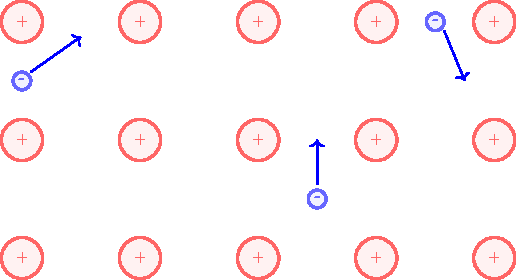
\includegraphics[scale=0.7]{Images/fig-solidcartoon.pdf}
    \caption{A cartoon visualization of a solid, here a square regular lattice with free electrons.}
    \label{fig-solidcartoon}
\end{figure}

\subsection{A Condensed Matter Theory of Everything}
Consider the Hamiltonian:
\begin{equation}
    H = \sum_i \frac{P_i^2}{2M} + \frac{(Ze)^2}{2}\sum_{i, i'}\frac{1}{\abs{\v{R}_i - \v{R}_{i'}}} + \sum_j \frac{p_j^2}{2m} + \frac{e^2}{2}\sum_{j, j'}\frac{1}{\abs{\v{r}_i - \v{r}_{i'}}} - Ze^2\sum_{i, j}\frac{1}{\abs{\v{R}_i - \v{r}_j}}.
\end{equation}
First term is ion KE, second term is ion-ion Coulomb interaction, third term is electron KE, fourth term is electron-electron Coulomb interaction, fifth term is ion-electron Coulomb interaction. This is in principle the theory of everything, which encompasses all that there is need to know in a solid. Note that spin is missing here; we should add two copies of everything (spin up, spin down) and relativistic effects (spin orbit coupling) but for most solids these are relatively small corrections. However, there is a large problem; this is a largely intractable problem. The main problem is that $N$ (the number of electrons in a given solid) is extremely large; $N \sim 10^{23}$. Let's consider some cases of $N$.
\begin{itemize}
    \item $N = 1$ is the hydrogen atom; this has been solved by Schrodinger (and in undergraduate QM) exactly.
    \item $N = 2$ is the Helium atom; already there exists no exact solution. But there are approximate methods that work well (e.g. variational principle for finding the ground state energy)
    \item $N = 1-100$ is the whole of chemistry; there are more sophisticated approximation techniques here.
    \item $N \sim 10^{23}$ is the theory of solids.
\end{itemize}
The key issue of the problem is the size of the corresponding Hilbert space is \emph{enormous}. It's even hard to estimate how large, as position and momentum are continuous. But just to illustrate the size of $\H$ for $N = 10^{23}$, let's consider a simpler setting where we only consider spin and ignore all of the motional degrees of freedom. For spin, there are two states; $\uparrow$ and $\downarrow$ per electron. So the total number of basis states is $2^{N} = 2^{10^{23}} \approx 10^{10^{23}/3}$. There is no computer possible that can store this much information! In fact as an amusing comparison, there are only $3.8 \times 10^{50}$ atoms on Earth, $1.2 \times 10^{57}$ atoms on the sun, and $1.3 \times 10^{79}$ atoms in the visible universe; our brute force method is destined to fail. Our conclusion is that drastic approximations are required in order to make progress in any valid description of solids. And note that they may be drastic, but these approximations turn out to be quite good; there is some simplicity that emerges from what seems to be a hopelessly large and complex Hilbert space. We can achieve a very good understanding of many things; e.g. the physics necessary to construct the device on which this document was written.

\subsection{The Born-Oppenheimer Approximation}
The Born-Oppehnheimer, or adiabatic approximation was originally developed as an approximation method to describe complex molecules; however it applies to our current discussion of solids. It is based on the observation that $M \gg m$ (where $M$ is the ion mass and $m$ the electron mass), namely $\frac{m}{M} \sim 10^{-3}-10^{-5}$. We imagine that in a complicated system of electrons and ions we have equipartition of energy\footnote{Equipartition is a result from classical physics, but it applies suprisingly well.}; because the energy scales of electrons and ions are comparable, the electrons will be moving much faster. Therefore it is possible to decouple the problem of electrons and phonons, by solving the electron motion on a static background of ions. 

One can deduce that $v_{ion} \sim \left(\frac{m}{M}\right)^{3/4}v_F \sim 10^{-2}-10^{-3}v_F$. Also, $v_F \sim 3 \times 10^{6}\si{m/s} \sim 10^{-2}c$ so the physics we consider is non-relativistic (and we can add corrections to the order of 1\%). There are various supposedly intuitive arguments for why we have a power of $3/4$ on $\frac{m}{M}$, but most are not at all obvious or really reasonable; we will derive it after going further into our discussion of solids.

We explore the consequences of $v_{ion} \ll v_F$ for solutions of the Schrodinger equation:
\begin{equation}\label{eq-SE}
    H\psi(\v{r}, \v{R}) = E\psi(\v{r}, \v{R})
\end{equation}
where $\v{r} = \set{\v{r}_j}_j$ and $\v{R} = \set{\v{R}_i}_i$. We make the ansatz:
\begin{equation}
    \psi(\v{r}, \v{R}) = \sum_n \phi_n(\v{R})\psi_{e, n}(\v{r}, \v{R})
\end{equation}
where $\psi_{e, n}$ are solutions to the \emph{electron} problem at fixed ion positions. In other words:
\begin{equation}\label{eq-fixedionansatz}
    \boxed{(T_e + V_{ee} + V_{ei})\psi_{e, n}(\v{r}, \v{R}) = E_{e, n}(\v{R})\psi_{e, n}(\v{r}, \v{R})}
\end{equation}
This in itself is an intractable problem, but it will be useful for our analysis to assume a solution of this form. Let us substitute our ansatz into the SE. We then obtain:
\begin{align*}
    (T_i + T_e + V_{ii} + V_{ee} + V_{ei})\psi = E\psi.
\end{align*} 
We can rewrite this as:
\begin{align*}
    (T_i + V_{ii})\psi + \sum_n \phi_n(T_e + V_{ee} + V_{ei})\psi_{e, n} = E\psi
\end{align*}
But the term in brackets of the sum if the electronic part, so:
\begin{equation}
    (T_i + V_{ii})\psi + \sum_n E_{e, n}(\v{R})\psi_{e, n}(\v{r}, \v{R}) = E\psi
\end{equation}
We can not multiply by $\psi^{*}_{e, m}(\v{r}, \v{R})$ and integrate over $\v{r}$. We then have many simplifications that arise from orthonormality (namely in the second term and the RHS). But the first term on the RHS is nontrivial as $T_i$ contains $\nabla_{\v{R}}$. In any case, we are left with:
\begin{equation}
    \sum_n \int d\v{r}\psi^*_{e, m}(\v{r}, \v{R})T_i \phi_n(\v{R})\psi_{e, n}(\v{r}, \v{R}) + (V_{ii} + E_{e, m}(\v{R}) - E)\phi_M(\v{R}) = 0.
\end{equation}
where we have used the orthonormality of $\psi_{e, n}$ to collapse most of the terms. Let us now analyze the troublesome term. We rewrite this as $\sum_{i}\bra{em}\frac{P_i^2}{2M}\phi_n(\v{R})\ket{en}$. $P_i^2$ is a second derivative, so we end up getting three terms; one term where both derivatives act on $\phi_n$, a term where one acts on $\phi_n$ and the other on $\ket{en}$, and the last where both act on $\ket{en}$. Explicitly, we can write it as:
\begin{equation}\label{eq-problematicterm}
    \sum_{i}\bra{em}\frac{P_i^2}{2M}\phi_n(\v{R})\ket{en} = -\frac{\hbar^2}{2M}\sum_i \int d\v{r}\psi^*_{e, m}(\v{r}, \v{R})\left[(\nabla_{R_i}^2\phi_n(\v{R})) + 2(\nabla_{R_i}\phi_n(\v{R}))\nabla_{R_i} + \phi_n(\v{R})\nabla_{R_i}^2\right]\psi_{e, n}(\v{r}, \v{R}).
\end{equation}
The first term can be evaluated (as before) using orthonomality. The other two are not as convenient, but in the B-O approximation we may neglect the other two terms (and we will discuss shortly why this is a good idea).

We obtain the following equation:
\begin{equation}\label{eq-phononeq}
    \boxed{[T_i + V_{ii} + E_{e, n}(\v{R})]\phi_n(\v{R}) = E_n\phi_n(\v{R})}
\end{equation}

Note we can solve Eq. \eqref{eq-fixedionansatz} assuming the ions are static/in fixed positions. From there we obtain $E_{e, n}(\v{R})$ which allows us to solve Eq. \eqref{eq-phononeq} (which is known as a phonon equation), which allows us to obtain $E_n$ and $\phi_n(\v{R})$, which gives us the solution of the whole problem. We have decoupled one very complex problem into two connected but separately solvable equations. $E_{e, n}(\v{R})$ is called the effective ionic potential; without it a crystal would blow apart (via repulsive interaction), but it holds things together. 

As a last step, we must still demonstrate that the two neglected terms in \eqref{eq-problematicterm} make negligible contributions. One can show that:
\begin{enumerate}
    \item The first term is order $\left(\frac{m}{M}\right)^{1/2}\e_F$.
    \item The second term is order $\left(\frac{m}{M}\right)^{3/4}\e_F$.
    \item The third term is order $\left(\frac{m}{M}\right)\e_F$.
\end{enumerate}

However these estimates are for now opaque; we will confirm them later by further analysis. For now though, we recall that $\frac{m}{M} \sim 10^{-3}-10^{-5}$ so the second/third terms tend to be at least an order of magnitude smaller than the first (and can be neglected to first order). However, some important properties of crystalline solids are actually derived from these terms. For example if we analyze how electron motion couples to lattice vibration, then we have to start to worry about them. Additionally, the terms also contribute to resistivity of metals (phonon-electron scattering, especially important at high temperatures; why resistivity drops at lower temps)

So to start, we will study the electron and lattice degrees of freedom separately, but as we go further into our study we will have to revisit these coupling terms. Next week,
\newpage
\section{Second Quantization}
\subsection{Motivation}
The goal is to re-state the familiar Schrodinger equation:
\begin{equation}\label{eq-se}
    i\hbar\dpd{}{t}\psi(\v{x}_1, \ldots, \v{x}_N, t) = H\psi(\v{x}_1, \ldots, \v{x}_N, t).
\end{equation}
in a more convenient format for $N \sim 10^{23}$. Second quantization is a bit of a misnomer; we will not quantize any further, but we will just recast the SE into a more convenient basis. Here we will give a summary of the derivation, and the gory mathematical details left to self-study; refer to the Chapter 1 handout of Fetter and Walecka.

We will consider the following Hamiltonian as an example:
\begin{equation}
    H = \sum_{k=1}^N T(\v{x}_k) + \frac{1}{2}\sum_{k < l}^N V(\v{x}_k, \v{x}_l)
\end{equation}
where we have the single-particle operator $T$ (kinetic energy) and the two-particle operator $V$ (interaction; e.g. Coulomb).

\subsection{The Central Idea}
The problem is that the number of variables that this wavefunction depends on is absolutely astronomical. The key will be that any two electrons are \emph{fundamentally indistinguishable}; instead of keeping track of $N \sim 10^{23}$ positions, it is sufficient to specify how many particles occupy a given single-particle state. To this end we choose a basis of single particle states $\psi_{E_k}(\v{x}_k)$ where $E_k$ represents a complete set of single-particle quantum numbers\footnote{$E_k$ does \emph{not} represent energy} (e.g. momentum $\v{p}$ for spinless bosons in a 3d box, or $n, l, m, s_z$ for an electron in a hydrogen atom). We then write the many-body wavefunction in this basis as:
\begin{equation}
    \psi(\v{x}_1, \ldots, \v{x}_N, t) = \sum_{E_1, \ldots, E_N}C(E_1, \ldots, E_N, t)\psi_{E_1}(\v{x}_1)\ldots \psi_{E_N}(\v{x}_N)
\end{equation}
We must distinguish two possible cases for these particles; namely they can either be bosons or fermions i.e. take care of the ``exchange statistics''. This is encoded in the many body wavefunction as a property of how the wavefunction behaves under exchange of any two particles:
\begin{equation}
    \psi(\ldots, \v{x}_i, \ldots, \v{x}_j, \ldots, t) = \pm \psi(\ldots, \v{x}_j, \ldots, \v{x}_i, \ldots, t)
\end{equation}
with $+$ corresponding to bosons and $-$ corresponding to fermions. This has far-reaching consequences for the nature of many-body states. If this wavefunction rule is obeyed, the coefficients must obey the same rule:
\begin{equation}
    C(\ldots, E_i, \ldots, E_j, \ldots, t = \pm C(\ldots, E_j, \ldots, E_i, \ldots, t).
\end{equation}
Bosons are a bit easier, so we discuss them first.

\subsection{The Boson Case}
For the sake of simplicity, we will imagine that the $E_j$s are represented by integers, namely $E_j \in \NN$. Suppose we have coefficient $C(12134115\ldots, t)$. Since we are free to exchange any of the integers as we like, we may arrange it as:
\begin{align*}
    C(12134115\ldots, t) = C(1111\ldots 2222\ldots 333\ldots \ldots, t)
\end{align*}
where we have $n_1$ $1$s, $n_2$ $2$s, $n_3$ $3$s and so on. 
It should be immediately clear that it is not necessary to keep track of all $10^{23}$ numbers, but just the number of particles in each state (each number). We then define:
\begin{equation}
    C(1111\ldots 2222\ldots 333\ldots \ldots, t) \equiv \bar{C}(n_1, n_2, \ldots, n_\infty, t).
\end{equation}
In analogy, when we think about our bank account, we do not care about the individual dollars or what they look like; we only care about the total number of dollars in each of our accounts. We can then write the wavefunction in terms of $\bar{C}$, and then massage the resulting expressions to obtain convenient equations (as is done in the text).

\subsection{Many-Body Hilbert Space, Creation/Annhilation Operators}
We introduce a many-body Hilbert space and creation/annhilation operators that act on states in the space. States in the space look like. These states are orthonormal and complete:
\begin{equation}
    \begin{split}
        &\braket{n_1'n_2'\ldots n_\infty'}{n_1n_2\ldots n_\infty} = \prod_{i=1}^\infty \delta_{n_i, n_i'}
        \\ &\sum_{n_1, n_2, \ldots, n_\infty} \ket{n_1n_2\ldots n_\infty}\bra{n_1n_2\ldots n_\infty} = 1.
    \end{split}
\end{equation}
We then define the creation/annhilation operators by defining their commutation relations. For bosons, we have:
\begin{equation}
    \begin{split}
        [b_k, b_{k'}^\dagger] &= \delta_{kk'}
        \\ [b_k, b_{k'}] &= 0
        \\ [b_k^\dagger, b_{k'}^\dagger] &= 0
    \end{split}
\end{equation}
where $b_k^\dagger$ is said to create a boson in state $\psi_{E_k}(\v{x})$. We record the notation:
\begin{equation}
    \ket{n_1n_2\ldots n_\infty} = \ket{n_1}\otimes\ket{n_2}\otimes\ldots\otimes\ket{n_\infty}.
\end{equation}

We can now use the commutation relations to count the number of particles, as well as create and annhilate them:
\begin{equation}
    \begin{split}
        b_k^\dagger b_k \ket{n_k} &= n_k\ket{n_k}
        \\ b_k\ket{n_k} &= \sqrt{n_k}\ket{n_k - 1}
        \\ b_k^\dagger \ket{n_k} &= \sqrt{n_k + 1}\ket{n_k + 1}.
    \end{split}
\end{equation}
and if there is no boson to destroy (i.e. we have the vacuum state $\ket{0}$), we have the special case of:
\begin{align*}
    b_k\ket{0} = 0.
\end{align*}
Most of the states of interest in CM physics is low-temperature states where there are limited number of states with large occupancies. E.g. Bose-Einstein condensation, where all particles go into the single-particle ground state ($n_1$ is huge, $n_i$ for $i > 1$ are zero). When you heat up this condensate a little, $n_1$ will still be large, and the excited states will start to be occupied.

\subsection{Second Quantization Result}
With these definitions, one can show (see F\&W) that Eq. \eqref{eq-se} becomes:
\begin{equation}
    \begin{split}
        &i\hbar \dpd{}{t}\ket{\psi(t)} = H\ket{\psi(t)}
        \\ &\boxed{H = \sum_{i, k}\bra{i}T\ket{j}b_i^\dag b_j + \frac{1}{2}\sum_{ijkl} \bra{ij}V\ket{kl}b_i^\dag b_j^\dag b_l b_k}.
    \end{split}
\end{equation}
Note the order of $b_lb_k$ above. This does not matter for bosons (as the two are seen to commute via the commutation relations), but it will matter for fermions, as we will soon see. As a reminder, $\ket{\psi(t)}$ lives in the many-body Hilbert space:
\begin{align*}
    \ket{\psi(t)} = \sum_{n_1n_2\ldots n_\infty}f(n_1, n_2, \ldots, n_\infty, t)\ket{n_1n_2\ldots n_\infty}.
\end{align*}
In second quantization, the important quantities of interest to calculate will be the matrix elements of $T$ and $V$ with respect to the chosen multi-particle basis.

\subsection{The Fermion Case}
For fermions, the anti-symmetry under exchange implies the Pauli exclusion principle; that is, at most one fermion can occupy a given state. To see this in terms of the coefficients $C$, we have the relation:
\begin{equation}
    C(11\ldots) = -C(11\ldots)
\end{equation}
where we have interchanged the $1$s. The only way this can be satisfied is if $C(11\ldots) = 0$. So for the coefficient to be nonzero, all of the fermions must be in different states. In second quantization, this is implemented by the anti-commutation relations of creation and destruction operators:
\begin{equation}
    \begin{split}
        \{c_s, c_{s'}^\dagger\} &= \delta_{kk'}
        \\ \{c_s, c_{s'}\} &= 0
        \\ \{c_s^\dagger, c_{s'}^\dagger\} &= 0
    \end{split}
\end{equation}
Where $\{A, B\} = AB + BA$ is the anticommutator. We can derive the following properties:
\begin{enumerate}
    \item $\{c_s^\dag, c_s^\dag\} = 2c_s^\dag c_s^\dag = 0$, so:
    \begin{equation}
        c_s^{\dag 2} = 0 \implies c_s^{\dag 2}\ket{0} = 0
    \end{equation}
    this is a restatement of the Pauli principle. We cannot create two fermions in the same state. Analogously, $c_s^2 = 0$.
    \item We have the number operator (as in the boson case) of $\hat{n} = c^\dag c$. We then have that:
    \begin{equation}
        (\hat{n})^2 = (c^\dag c)^2 = c^\dag c c^\dag c = c^\dag (1 - c^\dag c)c = c^\dag c = \hat{n}
    \end{equation}
    where in the second-to-last equality we use the anticommutation relation and for the last equality we use that $c^{\dag 2} = 0$. So, the number operator has the property of idempotency. From this we can conclude that $\hat{n}$ has eigenvalues of $0$ and $1$ (as these are the only values that square to 1). This again is consistent with the Pauli exclusion principle; either we have zero or one fermions in a given quantum state.
    \item It is easy to deduce:
    \begin{equation}
        \begin{split}
            &c^\dag\ket{0} = \ket{1} \quad c\ket{1} = \ket{0}
            \\ &c^\dag\ket{1} = c^\dag c^\dag \ket{0} = 0
            \\ &c\ket{1} = c c\ket{0} = 0
        \end{split}
    \end{equation}
\end{enumerate}

A note with bookkeeping; because of the anti-commutation rules, it becomes necessary to track signs in many-body states. We have the following many-particle state which we apply $c_s$ to:
\begin{equation}
    \begin{split}
        &\ket{n_1n_2 \ldots n_\infty} = (c_1^\dag)^{n_1}(c_2^\dag)^{n_2} \ldots (c_\infty^\dag)^{n_\infty}\ket{0}.
        \\  &c_s\ket{n_1n_2\ldots n_\infty} = (-1)^{s_s}(c_1^\dag)^{n_1}(c_2^\dag)^{n_2} \ldots (c_sc_s^\dag)\ldots (c_\infty^\dag)^{n_\infty}\ket{0}
    \end{split}
\end{equation}
where $s_s = \sum_{i=1}^{s-1} n_i$; the sign has been accumulated by pushing the $c_s$ through. This implies the following rules for many-body fermion states:
\begin{equation}
    \begin{split}
        &c_s\ket{\ldots n_s \ldots} = \begin{cases}
            (-1)^{s_s}\sqrt{n_s}\ket{\ldots n_{s} - 1 \ldots} & \text{if $n_s = 1$}
            \\ 0 & \text{if $n_s = 0$}
        \end{cases}
        \\ &c_s^\dag\ket{\ldots n_s \ldots} = \begin{cases}
            (-1)^{s_s}\sqrt{n_s+1}\ket{\ldots n_{s} + 1 \ldots} & \text{if $n_s = 0$}
            \\ 0 & \text{if $n_s = 1$}
        \end{cases}
        \\ &c_s^\dag c_s\ket{\ldots n_s \ldots} = n_s\ket{\ldots n_s \ldots}.
    \end{split}
\end{equation}
Note however the quantities in square roots are always one, so we can just forget about them.

Similar to bosons, we can rewrite Eq. \eqref{eq-se} as:
\begin{equation}
    \begin{split}
        &i\hbar\dpd{}{t}\ket{\psi(t)} = H\ket{\psi(t)}
        \\ &H = \sum_{rs}\bra{r}T\ket{s} c_r^\dag c_s + \frac{1}{2}\sum_{rstn}\bra{rs}V\ket{tu} c_r^\dag c_s^\dag c_u c_t.
    \end{split}
\end{equation}
where we again note the order of the annhilation operators.

\subsection{Field Operators}
It is often convenient to create a particle at a point $\v{x}$ To this end, we define field operators:
\begin{equation}
    \hat{\psi}(\v{x}) = \sum_k \psi_k(\v{x})c_k, \quad \hat{\psi}^\dag(\v{x}) = \sum_k \psi_k^\dag(\v{x})c_k^\dag
\end{equation}
These can be viewed as a kind of Fourier transform, or more generally as a change of basis. As an example, consider spin-1/2 fermions. We can label them by the momentum $\v{k}$ and the spin $s_z$. The index $k$ can be thought as $k = (\v{k}, s_z)$. Then, $\psi_k(\v{x})$ can be thought of as two-component spinors, where:
\begin{equation}
    \psi_k(\v{x}) = \m{\psi_\v{k}(\v{x})_1 \\ \psi_\v{k}(\v{x})_2}
\end{equation}
which can be thought of the wavefunctions for the spin up and down projections. We can easily deduce commutation (and anti-commutation) relations for the field operators:
\begin{equation}
    \begin{split}
        &[\hat{\psi}_\alpha(\v{x}), \hat{\psi}_\beta^\dag(\v{x}')]_\pm = \sum_k \psi_k(\v{x})_\alpha \psi_k(\v{x}')_\beta^* = \delta_{\alpha\beta}\delta(\v{x} - \v{x}').
        \\ &[\hat{\psi}_\alpha(\v{x}), \hat{\psi}_\beta(\v{x}')]_\pm = [\hat{\psi}^\dag_\alpha(\v{x}), \hat{\psi}^\dag_\beta(\v{x}')]_\pm = 0
    \end{split}
\end{equation}
Similarly, the Hamiltonian can be written as:
\begin{equation}
    H = \int d^3x \hat{\psi}^\dag(\v{x})T(\v{x})\hat{\psi}(\v{x}) + \frac{1}{2}\int d^3xd^3y \hat{\psi}^\dag(\v{x})\hat{\psi}^\dag(\v{y}) V(\v{x}, \v{y})\hat{\psi}(\v{y})\hat{\psi}(\v{x}).
\end{equation}
and we invite the reader to check that this is indeed the case. Note that in general there should always be the same number of creation and annhilation operators; except towards the end of the course when we will look at superconducting systems, where there will be more creation than annhilation (and we will think about how to understand this). There are other operators that can be discussed in the same way. 
\begin{enumerate}
    \item The current operator. The form of the operator in first and second quantization is given below:
    \begin{equation}
        \begin{split}
            J(\v{x}) &= \sum_{i=1}^N J(\v{x}_i)
            \\ \hat{J} &= \sum_{rs}\bra{r}J\ket{s}c_r^\dag c_s = \int d^3x \sum_{rs} \psi_r^\dag(\v{x}) J(\v{x})\psi_s(\v{x})c_r^\dag c_s = \int d^3 x \hat{\psi}^\dag(\v{x})J(\v{x})\hat{\psi}(\v{x})
        \end{split}
    \end{equation}
    We see why the second quantization notation is so useful/economical; we simply take the first-quantized operator, sandwhich it between field operators, and integrate.
    \item The number operator. This follows much of the same logic as the current operator above. The first expression gives the number density, and the second the total particle number (which is obtained by integrating the number density over all space).
    \begin{equation}
        \begin{split}
            \hat{n}(\v{x}) &= \sum_{r, s} \psi_r^\dag(\v{x})\psi_s(\v{x})c_r^\dag c_s = \hat{\psi}^\dag(\v{x})\hat{\psi}(\v{x})
            \\ \hat{N} &= \int d^3x \hat{n}(\v{x}) = \int d^3x\hat{\psi}^\dag(\v{x})\hat{\psi}(\v{x}).
        \end{split}
    \end{equation}
\end{enumerate}
\newpage
\section{Degenerate Electron Gas}
The office hours for this course will be Monday 4-5pm with Marcel, and 4-5pm on Tuesday with Oguzhan.

\subsection{Introducing the Degenerate Electron Gas}
\begin{figure}[htbp]
    \centering
    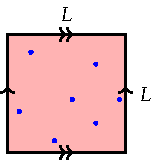
\includegraphics[]{Images/fig-jelliumcartoon.pdf}
    
    \caption{A cartoon depiction of the degenerate electron gas model. We consider a fixed, finite number of electrons $N$ in a three-dimensional box with side length $L$ and periodic boundary conditions. The electrons feel a uniformly distributed background of positive charge.}
    \label{fig-jelliumcartoon}
\end{figure}
Also known as the ``Jellium Model'', we consider a gas of electrons moving in a uniformly distributed background of positive charge. We begin with a 3d box of size $L$, and then take the thermodynamic limit of $L \to \infty$. 

We will use periodic boundary conditions, so if an electron leaves the box from one side, it comes in from the other. This is convenient as then the model admits plane waves solutions. We could use hard boundaries, and the description should agree in the $L \to \infty$ limit, but this set of boundary conditions is harder to work with; we would have cosine and and sines instead of plane waves.

The plane-wave basis will be a natural choice given the periodic BCs. Explicitly, we can write this as:
\begin{equation}
    \psi_{k, \lambda}(\v{x}) = \frac{1}{\sqrt{V}}e^{i\v{k} \cdot \v{x}}\eta_\lambda
\end{equation}
with $\lambda = (\uparrow, \downarrow)$ is the spin index. We have the spinors:
\begin{equation}
    \eta_\uparrow = \m{1\\0}, \quad \eta_\downarrow = \m{0\\1}
\end{equation}
The momentum is given by:
\begin{equation}
    \v{k} = (k_x, k_y, k_z), k_i = \frac{2\pi}{L}n_i
\end{equation}
where $n_i \in \ZZ$. The Hamiltonian is given by:
\begin{equation}
    \begin{split}
        H &= H_{el} + H_b + H_{el-b}
        \\ H_{el} &= \sum_{i=1}^N \frac{p_i^2}{2m} + \frac{1}{2}e^2\sum_{i \neq j} \frac{e^{-\mu\abs{\v{r}_i - \v{r}_j}}}{\abs{\v{r}_i - \v{r}_j}}
        \\ H_b &= \frac{1}{2}e^2 \int d^3x d^3x' \frac{n(\v{x})n(\v{x}')e^{-\mu\abs{\v{x} - \v{x}'}}}{\abs{\v{x} - \v{x}'}}
        \\ H_{el-b} &= -e\sum_{i=1}^N \int d^3x \frac{n(\v{x})e^{-\mu\abs{\v{x} - \v{r}_i}}}{\abs{\v{x} - \v{r}_i}}.
    \end{split}
\end{equation}
$H_{el}$ is just the kinetic energy of the electrons and the point-charge on point-charge interactions. $H_b$ is the electrostatic interaction of the background field with itself. And $H_{el-b}$ is the electrostatic interactions of the electrons with the background field. $N$ is the number of electrons, $V = L^3$ is the volume, $n = N/V$ is the electron density, and $\mu$ is a convergence factor which we send $\mu \to 0$\footnote{In nuclear physics this has significance as the \emph{Yukawa potential}; here we just use it as a convenient trick to remove some diverging integrals}. 

\subsection{Simplifying the background terms}
We want to rewrite this in second quantization notation. Only $H_e$ will have nontrivial structure in the second quantization notation, but nevertheless the other terms are necessary for the stability of the system.

Let us start with the second term, which is the simplest. We deal with a uniform background density, namely $n(\v{x}) = n = N/V$. $H_b$ then becomes a simple integral:
\begin{equation}
    \begin{split}
        H_b &= \frac{1}{2}e^2\left(\frac{N}{V}\right)^2 \int d^3x \int d^3 x' \frac{e^{-\mu\abs{\v{x} - \v{x}'}}}{\abs{\v{x} - \v{x}'}}.
        \\ &= \frac{1}{2}e^2\left(\frac{N}{V}\right)^2 \int d^3x \int d^3z \frac{e^{-\mu z}}{z}
        \\ &= \frac{1}{2}e^{2}\left(\frac{N^2}{V}\right)\frac{4\pi}{\mu^2}
    \end{split}
\end{equation}
Where in the second equality we use $z = \v{x}' - \v{x}$ in order to make the integrals independent, and evaluate the integrals in the third equality (the inner integral evaluating to $\frac{4\pi}{\mu^2}$, the outer to $V$). We can see why it was useful to introduce the $e^{-\mu}$; the integral would have diverged otherwise due to the long-range nature of the Coloumb interaction. Note also that we performed the integral assuming $\mu^{-1} \ll L$. We can similarly calculate $H_{el-b}$:
\begin{equation}
    \begin{split}
        H_{el-b} &= -e\frac{N}{V}\sum_{i=1}^N \int d^3x \frac{e^{-\mu\abs{\v{x} - \v{r}_i}}}{\abs{\v{x} - \v{r}_i}}
        \\ &= -e\frac{N}{V}\sum_{i=1}^N \int d^3z \frac{e^{-\mu z}}{z}
        \\ &= -e^2 \frac{N}{V} N \int d^3z\frac{e^{-\mu z}}{z}
        \\ &= -e^2\frac{N^2}{V}\frac{4\pi}{\mu^2}
    \end{split}
\end{equation}
We note the partial cancellation of the $H_b$ and the $H_{el-b}$ terms of the Hamiltonian; we will see another cancellation later.

A reasonable question is why the $\mu^{-1} \ll L$ assumption is necessary. It boils down to the the fact that we have periodic boundary conductions, and we do \emph{not} want the electric field of a given electron to interact with itself (or at least, not in a way that is exponentially insignificant and hence ignorable). See Fig. \ref{fig-jelliumlengthassumption} below for a visual demonstration of the importance of this assumption.

\begin{figure}[htbp]
    \centering
    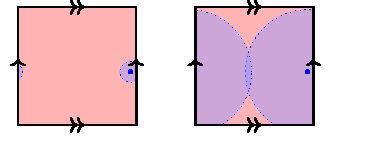
\includegraphics[]{Images/fig-jelliumlengthassumption.pdf}
    
    \caption{Comparisons of ``spheres of interaction'' of electrons when $\mu^{-1} \ll L$ (left) and $\mu^{-1} \sim L$ (right). We can see that in the former case, the electron does not interact with itself through the periodic boundary condition (beyond a negligeble exponentially small contribution), and so the system is physically sound. In the latter case, the electron does have a nontrivial interaction with its own electric field, as seen through the overlap of the sphere of interaction; this is not physical. Hence in our analysis of the Jellium model, we make the assumption that $\mu^{-1} \ll L$.}
    \label{fig-jelliumlengthassumption}
\end{figure}

With these simplifications, 
\begin{equation}
    H = -\frac{1}{2}e^2\frac{N^2}{V}\frac{4\pi}{\mu^2} + H_{el}
\end{equation}
Note that all of the interesting physics is contained in $H_{el}$, but we need $H_b + H_{el}$ to get a finite theory; we can see that if we took $\mu \to 0$ now, the energy would diverge; presumably there will be some sort of cancellation that occurs with $H_{el}$ that will regularize the theory. 

\subsection{Second Quantization of the Electron Term}
Let us now transform the $H_{el}$ term into second quantized notation.
\begin{enumerate}[(i)]
    \item We start with the kinetic energy term:
    \begin{equation}
        \begin{split}
            \bra{\v{k}_1\lambda_1}T\ket{\v{k}_2\lambda_2} &= \frac{1}{2mV}\int d^3x e^{-i\v{k} \cdot \v{x}}\eta_{\lambda_1}^\dag (-\hbar^2\nabla^2)e^{i\v{k}_2\cdot \v{x}}\eta_{\lambda_2}
            \\ &= \frac{\hbar^2 k_2^2}{2mV}\delta_{\lambda_1\lambda_2}\int d^3x e^{-i\v{x} \cdot (\v{k}_1 - \v{k_2})}
            \\ &= \frac{\hbar^2k_2^2}{2m}\delta_{\lambda_1\lambda_2}\delta_{\v{k}_1\v{k}_2}
        \end{split}
    \end{equation}
    where we use that $\int d^3x e^{-i\v{x} \cdot (\v{k}_1 - \v{k_2})} = V\delta_{k_1k_2}$. Wee therefore obtain:
    \begin{equation}
        \hat{T} = \sum_{k, \lambda}\frac{\hbar^2 k^2}{2m}c_{k\lambda}^\dag c_{k\lambda}.
    \end{equation}
    \item We now look at the potential term:
    \begin{equation}
        \bra{k_1\lambda_1k_2\lambda_2}V\ket{k_3\lambda_3k_4\lambda_4} = \frac{e^2}{V}\delta_{\lambda_1\lambda_3}\delta_{\lambda_2\lambda_4}\delta_{k_1 + k_2, k_3 + k_4}\frac{4\pi}{(\v{k}_1 - \v{k}_3)^2 + \mu}.
    \end{equation}
    See F\&W for details; there is nothing conceptually new in the calculation above, it is only slightly more annoying at there are four plane wave terms.
\end{enumerate}
We therefore obtain:
\begin{equation}\label{eq-JelliumquantizedH}
    \hat{H} = \hat{T} - \frac{1}{2}\frac{e^2N^2}{V}\frac{4\pi}{\mu} + \frac{e^2}{2V}\sum_{k, \lambda}\delta_{\lambda_1\lambda_3}\delta_{\lambda_2\lambda_4}\delta_{k_1 + k_2, k_3 + k_4}\frac{4\pi}{(\v{k}_1 - \v{k}_3)^2 + \mu} c^\dag_{k_1\lambda_1}c^\dag_{k_2\lambda_2}c_{k_4\lambda_4}c_{k_3\lambda_3}.
\end{equation}
Now we have to think a little bit; we have three delta functions, two for spin, one for momenta. We can explicitly two summations over $\lambda$ and one over momentum. Instead of doing so blindly, we will find it useful to make the following change of variables:
\begin{equation}
    \m{\v{k}_1 = \v{k} + \v{q} & \v{k}_3 = \v{k} \\ \v{k}_2 = \v{p} - \v{q} & \v{k}_4 = \v{p}} \quad \m{\lambda_1 = \alpha \\ \lambda_2 = \beta}
\end{equation}
We may notice that we express the four momenta in terms of three, but this is ok; we have the extra constraint on the momentum already, and it was designed to satisfy this constraint. Substituting, the potential term becomes:
\begin{equation}
    \frac{e^2}{2V}\sum_{\v{k}\v{p}\v{q}}\sum_{\alpha\beta}\frac{4\pi}{\v{q}^2 + \mu^2}c^\dag_{\v{k} + \v{q}\alpha}c^{\dag}_{\v{p} - \v{q}\beta}c_{\v{p}\beta}c_{\v{k}\alpha}.
\end{equation}
We now want to send $\mu \to 0$. Note that we can do this for any term in the sum for which $\v{q} \neq \v{0}$. The only singular term is $\v{q} = \v{0}$, so let us study that term:
\begin{equation}\label{eq-badtermJellium}
    \begin{split}
        \frac{e^2}{2V}\sum_{\v{k}\v{p}}\sum_{\alpha\beta}\frac{4\pi}{\mu^2}c^\dag_{\v{k}\alpha}c^{\dag}_{\v{p}\beta}c_{\v{p}\beta}c_{\v{k}\alpha} &= \frac{e^2}{2V}\sum_{\v{k}\v{p}}\sum_{\alpha\beta}\frac{4\pi}{\mu^2}c^\dag_{\v{k}\alpha}(c_{\v{k}\alpha}c^\dag_{\v{p}\beta} - \delta_{\v{k}\v{p}}\delta_{\alpha\beta})c_{\v{p}\beta}
        \\ &= \frac{e^2}{2V}\frac{4\pi}{\mu^2}(\hat{N}^2 - \hat{N})
        \\ &=\frac{e^2}{2}\frac{N^2}{V}\frac{4\pi}{\mu^2} - \frac{e^2}{2}\frac{N}{V}\frac{4\pi}{\mu^2}
    \end{split}
\end{equation}
where in the first equality we have commuted the $c_{\v{k}\alpha}$ between the two $c^\dag$s (being careful to respect the commutation relations), in the second equality we have used the definition of the number operator, and in the third equality we used the fact that we work with a system with a finite, fixed number of electrons and hence we can replace the operators $\hat{N}$ with the number of particles $N$. 

We see that the first term in Eq. \eqref{eq-badtermJellium} and the second term in Eq. \eqref{eq-JelliumquantizedH} cancel. We argue that the second term in Eq. \eqref{eq-badtermJellium} is vanishingly small in the thermodynamic limit. We argue this as follows; since $N/V$ (the number density) is constant with the system size, the term is constant with the system size; however $\avg{H}$ is extensive, and scales with the system size ($\avg{H} \sim V \sim N$). Hence we may choose to ignore it. So let us conclude by stating our final Hamiltonian:
\begin{equation}
    \hat{H} = \sum_{\v{k}\alpha}\frac{\hbar^2\v{k}^2}{2m}c^\dag_{\v{k}\lambda}c_{\v{k}\lambda} + \frac{e^2}{2V}\sum_{\v{k}\v{p}\v{q}}'\sum_{\alpha\beta} \frac{4\pi}{\v{q}^2}c^\dag_{\v{k} + \v{q}\alpha}c^{\dag}_{\v{p} - \v{q}\beta}c_{\v{p}\beta}c_{\v{k}\alpha}
\end{equation}
where the prime on the summation denotes that we do not include the $\v{q} = 0$ term.

\subsection{Rescaling the Hamiltonian}
It is possible to gain important insights by introducing ``natural'' dimensionless variables. We define the inter-electron spacing $r_0$ as the radius of the sphere corresponding to the volume per electron. We then define the dimensionless quantity $r_s$ as the ratio of $r_0$ with the Bohr radius $a_0$:
\begin{equation}
    \begin{split}
        &\frac{V}{N} = \frac{4}{3}\pi r_0^3
        \\ &a_0 = \frac{\hbar^2}{me^2}
        \\ &\boxed{r_s = \frac{r_0}{a_0} \approx 2-6 \text{ for metals}}
    \end{split}
\end{equation}
The above are very good things to remember; there will be questions about them on the midterm and final!
Based on these, let us define:
\begin{equation}
    \bar{V} = V/r_0^3, \bar{\v{k}} = \v{k}r_0
\end{equation}
So our rescaled Hamiltonian can be written as:
\begin{equation}
    \hat{H} = \frac{e^2}{a_0r_s^2}\left(\sum_{\bar{\v{k}}\alpha} \frac{\bar{\v{k}}^2}{2}c^\dag_{\bar{\v{k}}\lambda}c_{\bar{\v{k}}\lambda} + \frac{e^2}{2\bar{V}}\sum_{\bar{\v{k}}\bar{\v{p}}\bar{\v{q}}}'\sum_{\alpha\beta} \frac{4\pi}{\bar{\v{q}}^2}c^\dag_{\bar{\v{k}} + \bar{\v{q}}\alpha}c^{\dag}_{\bar{\v{p}} - \bar{\v{q}}\beta}c_{\bar{\v{p}}\beta}c_{\bar{\v{k}}\alpha}\right)
\end{equation}
where $\frac{e^2}{a_0} \approx 13.6\si{eV}$ is the Rydberg constant/hydrogen binding energy. This result shows that \underline{in the $r_s \to 0$} \underline{(high density) limit, the electron-electron interaction becomes weak.} This is very counterintutive; in classical physics, the electron-electron interaction would dominate! Another thing to note; starting from the high-density limit, we can solve an easy problem (one that just contains the kinetic energy of the electrons) and then treat the electron-electron interactions as a small perturbation (can be reasonably treated in perturbation theory, expanding in powers of $r_s$). The actual series for the ground-state energy reads:
\begin{equation}
    E_G = \frac{Ne^2}{a_0r_s^2}\left(a + br_s + cr_s^2 \log(r_s) + dr_s^2 + \cdots\right)
\end{equation}
the $\log(r_s)$ term is perhaps a bit peculiar, but indeed if we do the perturbation expansion diligently we can confirm that it shows up. In the following, we will find $a$ and $b$. We also remark that $c$ may be similarly obtained, but $d$ and higher powers require more advanced techniques, namely Green's function techniques\footnote{Green's functions give us a way to do a more formalized version of perturbation theory. With them, the expansion has been computed to seventh order; but the computation becomes much more difficult as we add higher order terms.}. We now proceed with the perturbation theory.

\subsection{Perturbation Theory (High Density)}
We return to our non-rescaled Hamiltonian so as to avoid having to write bars all the time. We split the Hamiltonian into two parts (the kinetic energy term and the perturbing electron-electron term):
\begin{equation}
    \begin{split}
        \hat{H}_0 &= \sum_{\v{k}\alpha}\frac{\hbar^2\v{k}^2}{2m}c^\dag_{\v{k}\lambda}c_{\v{k}\lambda}
        \\ \hat{H_1} &= \frac{e^2}{2V}\sum_{\v{k}\v{p}\v{q}}'\sum_{\alpha\beta} \frac{4\pi}{\v{q}^2}c^\dag_{\v{k} + \v{q}\alpha}c^{\dag}_{\v{p} - \v{q}\beta}c_{\v{p}\beta}c_{\v{k}\alpha}
    \end{split}
\end{equation} 

\subsubsection{Zeroth Order}
The ground state of $\hat{H_0}$ can be written as:
\begin{equation}
    \ket{F} = \prod_{\abs{\v{k}} < k_F} c^\dag_{\v{k} \uparrow}c^{\dag}_{\v{k}\downarrow}\ket{0}.
\end{equation}
For $N$ electrons, the Fermi momentum is determined by:
\begin{equation}
    N = \bra{F}\hat{N}\ket{F} = \sum_{\v{k}\lambda}\bra{F}n_{\v{k}\lambda}\ket{F} = \sum_{\v{k}\lambda}\theta(k_F - \abs{\v{k}}) = 2V\int \frac{d^3k}{(2\pi)^{3}}\theta(k_F - \abs{\v{k}}) = \frac{2V}{(2\pi)^3}\left(\frac{4}{3}\pi k_F^3\right) = \frac{V}{3\pi^2}k_F^3
\end{equation}
We have therefore obtained $k_F$ defined by electron density. In the above we have used the standard perscription:
\begin{equation}
    \frac{1}{V}\sum_{\v{k}} \to \int \frac{d^3k}{(2\pi)^3}
\end{equation}
and the step function:
\begin{align*}
    \theta(x) = \begin{cases}
        1 & x > 0
        \\ 0 & x < 0.
    \end{cases}
\end{align*}
We can now solve for $k_F$:
\begin{equation}
    k_F = \left(\frac{3\pi^2 N}{V}\right)^{1/3} = \left(\frac{9\pi}{4}\right)^{1/3}r_0^{-1} \approx 1.92 r_0^{-1}
\end{equation}
which tells us that $k_F$ is (up to a factor of order unity) equal to the inverse of $r_0$. One can use the above to relate conduction bands and $k_F$ to the lattice spacing, among other useful applications. So now doing the ground state energy calculation, we have:

\begin{equation}
    \begin{split}
        E^{(0)} = \bra{F}\hat{H}_0\ket{F} = \frac{\hbar^2}{2m}\sum_{\v{k}, \alpha}\bra{F}n_{\v{k}\alpha}\ket{F}\v{k}^2 = \frac{\hbar^2}{2m}\sum_{\v{k}, \alpha}\v{k}^2\theta(k_F - \abs{\v{k}}) &= \frac{\hbar^2}{2m}2\frac{V}{(2\pi)^3}\int d^3k \v{k}^2\theta(k_F - \v{k})
        \\ &= \frac{3}{5}\frac{\hbar^2k_F^2}{2m}N
        \\ &= \frac{3}{5}\e_F N
        \\ &= \left(\frac{e^2}{2a_0}\right)N\frac{2.21}{r_s^2}
    \end{split}
\end{equation}
where in the fourth equality the factor of 2 comes from the summation over spin, and the integral is performed by going into spherical coordinates. Again $\frac{e^2}{2a_0} = 13.6\si{eV}$ is the Rydberg constant. This tells us that for metals (i.e. $r_s \approx 2-6$), the energy of electrons is on the order of $\si{eV}$.

\subsubsection{First Order}
To first order, we simply calculate the expectation value:
\begin{equation}
    E^{(1)} = \bra{F}\hat{H}_1\ket{F} = \frac{e^2}{2V}\sum_{\v{k}\v{p}\v{q}}'\sum_{\alpha\beta}\bra{F}c^\dag_{\v{k} + \v{q}\alpha}c^{\dag}_{\v{p} - \v{q}\beta}c_{\v{p}\beta}c_{\v{k}\alpha}\ket{F}.
\end{equation}
The above is more complicated; we must deal with the four-fermion operator acting on the ground state. We can do this the hard way; we can substitute in the ground state and use commutation relations amongst the operators. Or, we can give a slick argument that does the same job but with less writing; let's do it this way. We start with a Fermi sphere filled with electrons. The annhilation operators can only remove two electrons from inside the spheres, and the creation operators can either create electrons where they are removed, or create them elsewhere. If they are created elsewhere, the state we end up with will be orthogonal to the ground state $\ket{F}$. So, the only nonvanishing constributions will come from the terms where the annhilation operators remove electrons from inside the sphere, and the creation operators fill back in the holes (giving us back $\ket{F}$, up to some prefactor).

\begin{figure}[htbp]
    \centering
    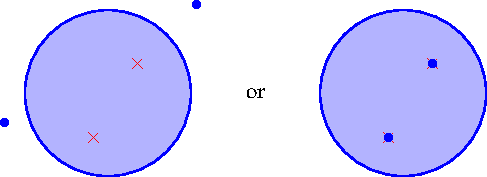
\includegraphics[]{Images/fig-fourfermionopargument.pdf}
    \caption{Action of the 4 fermion operators on the ground state $\ket{F}$. The two annihilation operators remove some pair of fermions within the Fermi sphere. The creation operators can then create fermions elsewhere (left), in which case the final state is orthogonal to $\ket{F}$ and does not contribute to the expectation value. Alternatively, the creation operators can fill the holes created by the annhilation operators (right), in which case the final state is proportional to $\ket{F}$ and hence does contribute to the expectation value.}
    \label{fig-fourfermionopargument}
\end{figure}

There are two pairings of the creation/annhilation operators for which the above can occur.  The first possibility is:
\begin{equation}
    \m{\v{k} + \v{q}, \alpha = \v{k}, \alpha
    \\ \v{p} - \v{q}, \beta = \v{p}, \beta} \quad \text{or} \quad \m{\v{k} + \v{q}, \alpha = \v{p}, \beta
    \\ \v{p} - \v{q}, \beta = \v{k}, \alpha}
\end{equation}
If we look at the first possibility, we immediately obtain the constraint that $\v{q} = 0$. However, we have already removed all such terms in our sum (note the prime); so the only the second possibility contributes. We call this the ``exchange term'', because the spins are exchanged. The conclusion of this argument is that the terms of the sum are only nonzero when the exchange conditions of $\v{k} + \v{q} = \v{p}, \alpha = \beta$ are satisfied. We can now use this to compute the first order correction to the GS energy:
\begin{equation}
    \begin{split}
        E^{(1)} &= \frac{e^2}{2V}\sum_{\v{k}\v{p}\v{q}}'\sum_{\alpha\beta} \delta_{\v{k} + \v{q}, \v{p}}\delta_{\alpha\beta} \bra{F}c^\dag_{\v{k} + \v{q}\alpha}c^{\dag}_{\v{p} - \v{q}\beta}c_{\v{p}\beta}c_{\v{k}\alpha}\ket{F}\frac{4\pi}{\v{q}^2}
        \\ &= \frac{e^2}{2V}\sum_{\v{k}\v{p}\v{q}}'\sum_{\alpha\beta} \delta_{\v{k} + \v{q}, \v{p}}\delta_{\alpha\beta} \bra{F}c^\dag_{\v{k} + \v{q}\alpha}c^{\dag}_{\v{k}\alpha}c_{\v{k} + \v{q}\alpha}c_{\v{k}\alpha}\ket{F}\frac{4\pi}{\v{q}^2}
        \\ &= -\frac{e^2}{2V}\sum'_{\v{k}\v{q}}
        \sum_\alpha\bra{F}\hat{n}_{\v{k} + \v{q} \alpha}\hat{n}_{\v{k}\alpha}\ket{F}\frac{4\pi}{\v{q}^2}
        \\ &= -\frac{e^2}{2V}\sum_{\v{k}\v{q}}'\sum_\alpha \frac{4\pi}{\v{q}^2}\theta(k_F - \abs{\v{k} + \v{q}})\theta(k_F - k)
        \\ &= -\frac{e^2}{2}\frac{4\pi V}{(2\pi)^6}\int d^3k \int d^3q\frac{1}{\v{q}^2} \theta(k_F - \abs{\v{k} + \v{q}})\theta(k_F - k)
    \end{split}
\end{equation}
We make a change of variables $\v{k} \to \v{p} = \v{k} + \frac{1}{2}\v{q}$. This yields:
\begin{equation}
    \begin{split}
        E^{(1)} &= -\frac{4\pi e^2V}{(2\pi)^6}\int d^3 q \frac{1}{\v{q}^2}\int d^3p \theta(k_F - \abs{\v{p} + \frac{1}{2}\v{q}})\theta(k_F - \abs{\v{p} - \frac{1}{2}\v{q}})
    \end{split}
\end{equation}
This integral is much more symmetric; if we think about this geometrically, we are looking at the overlap of spheres when we calculate the inner integral over $q$:

\begin{figure}[htbp]
    \centering
    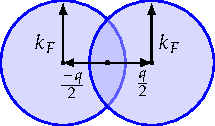
\includegraphics[]{Images/fig-twosphereoverlap.pdf}

    \caption{Visualization of the integral $I(q) = \int d^3p \theta(k_F - \abs{\v{p} + \frac{1}{2}\v{q}})\theta(k_F - \abs{\v{p} - \frac{1}{2}\v{q}})$. The two step functions correspond to the two spheres shown above, and the overall integral calculates their overlap in volume.}
    \label{fig-twosphereoverlap}
\end{figure}

The integral is a standard exercise in multivariable calculus. One finds:
\begin{equation}
    \int d^3p \theta(k_F - \abs{\v{p} + \frac{1}{2}\v{q}})\theta(k_F - \abs{\v{p} - \frac{1}{2}\v{q}}) = \frac{4\pi}{3}k_F^3\left(1 - \frac{3}{2}x + \frac{1}{2}x^2\right)\theta(1 - x), \quad x = \frac{q}{2k_F}.
\end{equation}
where the $\theta$ function is there to account for the fact that when $q$ is sufficiently large the spheres do not touch. We now calculate the outer integral. We make the observation that in spherical coordinates, $d^3q \to 4\pi q^2 dq$ and so the $q^2$ in the denominator cancels. All we have to do is just an integral of a polynomial; child's play. We are left with:
\begin{equation}
    E^{(1)} = -\frac{e^2}{2a_0}\frac{N}{r_s}\left(\frac{9\pi}{4}\right)^{1/2}\frac{3}{2\pi} = -\frac{e^2}{2a_0}N\frac{0.916}{r_s}.
\end{equation}

\subsubsection{Combining Results}
In summary, the total ground state energy (to first order) is:
\begin{equation}\label{eq-pertresultjellium}
    \frac{E}{N} = \frac{e^2}{2a_0}\frac{1}{r_s^2}\left(2.21 - 0.916r_S + \ldots\right)
\end{equation}
We identify the first term as the free Fermi gas energy, and the second term as the exchange energy.

A comment: We have done perturbation theory in $r_s$ which we have treated as ``small'', but really $r_s$ is $2-6$ for metals so it is not really small. It surprisingly works fairly well, anyway.

\subsection{The Variational Viewpoint}
We now switch perspectives a little bit, and find that we can learn something more interesting about the calculation we just did. We viewed it as a perturbation theory expansion in $r_s$. But we can view it instead as a variational calculation.

Recall the variational principle:
\begin{align*}
    E_{GS} \leq \bra{\psi}H\ket{\psi}
\end{align*}
where $H$ is a Hamiltonian, $\ket{\psi}$ is any state, and $E_{GS}$ is the ground state energy of $H$. In our case, we have calculated $\bra{F}\hat{H}_0 + \hat{H}_1\ket{F}$, which can also be viewed as a variational energy parametrized by electron density $r_s$. Taking our result from Eq. \eqref{eq-pertresultjellium}, we can plot an energy landscape as a function of $r_s$:

\begin{figure}[htbp]
    \centering
    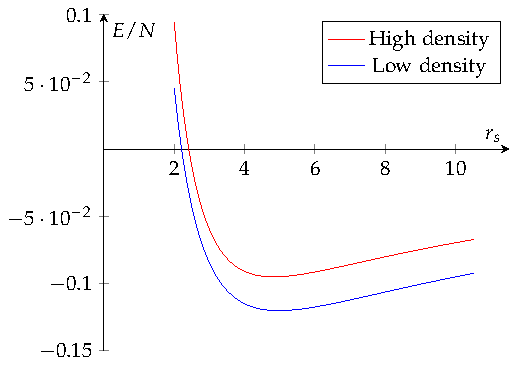
\includegraphics[]{Images/fig-jelliumenergylandscape.pdf}

    \caption{Plot of the variational energy landscape for. $E/N$ is in units of $e^2/2a_0$, and we plot in a range of typical $r_s$ for metals. In red we plot the first-order perturbation expansion for $E/N$ in the high-density limit (Eq. \eqref{eq-pertresultjellium}). In blue we plot the first-order perturbation expansion for $E/N$ in the low-density limit (Eq. \eqref{eq-pertresultjelliumlowdensity}). We can find the $r_s$ that minimizes $E/N$ to approximate the true ground state energy (i.e. the binding energy per electron in metals).}
    \label{fig-jelliumenergylandscape}
\end{figure}

We find that the $r_s$ that minimizes this energy is $(r_s)_{\min} = 4.83$ and $E_{\min}/N = -0.095\frac{e^2}{2a_0} \approx -1.29\si{eV}$. For comparison, the binding energy per electron in sodium (found experimentally) is $r_s = 3.86$ and $E/N = -1.13\si{eV}$. Even this very simple calculation gets us the correct order of magnitude.

\subsection{Perturbation Theory (Low Density)}
It turns out that we can do perturbation theory also in the large $r_s$/low-density limit, where we take:
\begin{align*}
    \hat{H}_0 &= \frac{e^2}{2V}\sum_{\v{k}\v{p}\v{q}}'\sum_{\alpha\beta} \frac{4\pi}{\v{q}^2}c^\dag_{\v{k} + \v{q}\alpha}c^{\dag}_{\v{p} - \v{q}\beta}c_{\v{p}\beta}c_{\v{k}\alpha}
    \\ \hat{H_1} &= \sum_{\v{k}\alpha}\frac{\hbar^2\v{k}^2}{2m}c^\dag_{\v{k}\lambda}c_{\v{k}\lambda}
\end{align*}
i.e. we exchange which is the dominant and which is the perturbing Hamiltonian. In this limit, we find (though the calculation is more difficult):
\begin{equation}\label{eq-pertresultjelliumlowdensity}
    \frac{E}{N} = \frac{e^2}{2a_0}\frac{1}{r_s}\left(-1.79 + \frac{2.66}{\sqrt{r_s}} + \ldots \right)
\end{equation}
This is plotted as the dashed line in the figure above. This is the controversial ``Wigner crystal''; it is not known if this actually applied, as the crystallization of electrons has never been observed in three dimensions.

Next class, we will look at the Hartree-Fock approximation.
\newpage
\setcounter{section}{4}
\section{The Hartree-Fock Approximation}
Note: Section 4 is not missing, but rather Degenerate Electron Gases spanned two lectures. 

\subsection{Motivation and Main Idea}
The Hartree-Fock, or mean-field approximation is useful when we have an intractable 4-fermion term in the Hamiltonian, for example the Coulomb interaction term.

The idea is quite simple. We approximate the full Hamiltonian $H = H_0 + H_1$ by the ``best possible'' approximation of the form:
\begin{equation}
    H_{HF} = \sum_{\v{k}, \alpha}\e_{\alpha}^{MF}(\v{k})c_{\v{k}\alpha}^\dag c_{\v{k}\alpha}.
\end{equation}
This looks like $H_0$ from before, but the modified dispersion relation allows for a tractable calculation.

\subsection{Heuristic Approach}
We first go for an intuitive approach, and then proceed with an approach that casts the problem in a variational setting (placing it on better footing). We consider:
\begin{equation}
    \begin{split}
        H_0 &= \sum_{\v{k}\alpha}\e_0(\v{k})c_{\v{k}\alpha}^\dag c_{\v{k}\alpha}
        \\ H_1 &= \frac{1}{2}\sum_{\v{kpq}\alpha\beta}V(\v{q})c^\dag_{\v{k} + \v{q}\alpha}c^\dag_{\v{p} - \v{q}\beta}c_{\v{p}\beta}c_{\v{k}\alpha}
    \end{split}
\end{equation}
Next, we ``decouple'' $H_1$ using the operator identity:
\begin{equation}
    AB = A\avg{B} + \avg{A}B - \avg{A}\avg{B} + (A - \avg{A})(B - \avg{B})
\end{equation}
This is useful as if we just focus on the last term, this is just the fluctuation of operator $A$ around its mean field value time the fluctuation of $B$ around its mean field value. The idea of mean-field theory is to say that the product of (small) fluctuations is small, and we therefore can neglect it. The central idea of the mean-field approach is to replace such products with the first three terms in the above operator identity.

Remark: in some sense, we assume that the fluctuations are small before we know what the solutions are, so we do not necessarily a priori know this will be the case. However, in practice this approach is greatly successful for the majority of problems in CM physics (the remaining 1\% of problems for which it fails tend to be interesting research problems).

Looking at our interaction term $H_1$, we have two ways to pair up our operators ($A = 13$ and $B = 24$ or $A = 14$ and $B = 23$). Let's go ahead with trying this simplification for our Hamiltonian.

\begin{equation}
    \begin{split}
        H_1^{MF} &= \frac{1}{2}\sum_{\v{kpq}\alpha\beta}V(\v{q})\left[c^\dag_{\v{k} + \v{q}\alpha}c_{\v{k}\alpha}\avg{c^\dag_{\v{p} - \v{q}\beta} c_{\v{p}\beta}} + \avg{c^\dag_{\v{k} + \v{q}\alpha}c_{\v{k}\alpha}}c^\dag_{\v{p} - \v{q}\beta} c_{\v{p}\beta} - \avg{c^\dag_{\v{k} + \v{q}\alpha}c_{\v{k}\alpha}}\avg{c^\dag_{\v{p} - \v{q}\beta} c_{\v{p}\beta}}\right.
        \\ &- \left.c^\dag_{\v{k} + \v{q}\alpha}c_{\v{p}\beta}\avg{c^{\dag}_{\v{p} - \v{q}\beta}c_{\v{k}\alpha}} - + \avg{c^\dag_{\v{k} + \v{q}\alpha}c_{\v{p}\beta}}c^{\dag}_{\v{p} - \v{q}\beta}c_{\v{k}\alpha} + \avg{c^\dag_{\v{k} + \v{q}\alpha}c_{\v{p}\beta}}\avg{c^{\dag}_{\v{p} - \v{q}\beta}c_{\v{k}\alpha}}\right]
    \end{split}
\end{equation}
Why do we include both pairings (the other pairings are dropped, but are zero in the Fermi sea)? Aren't we overcounting? In fact we are not (and careful thought shows this is not the case); this will become clearer when we do this variationally.

This looks intimidating, but there are some nice simplifications; we have two terms that come out:


for example, (s):
\begin{equation}
    \begin{split}
        \avg{c^{\dag}_{\v{p} - \v{q}\beta}c_{\v{p}\beta}} &= \delta_{\v{q} = 0}\avg{c^{\dag}_{\v{p}\beta}c_{\v{p}\beta}}
        \\ \avg{c^{\dag}_{\v{p} - \v{q}\beta}c_{\v{k}\alpha}} &= \delta_{\alpha\beta}\delta_{\v{p} - \v{q} = \v{k}}\avg{c^{\dag}_{\v{p}\beta}c_{\v{p}\beta}}
    \end{split}
\end{equation}
where the delta shows up as the product vanishes unless we are looking at the same spin with the same momentum. The first line is the direct, or \emph{Hartree} term. The second line is the exchange, or \emph{Fock} term. Taking into account these simplifications, the mean field for the Hartree-Fock Hamiltonian takes the form:
\begin{equation}
    H^{MF} = \sum_{\v{k}\alpha}\left[\e_{0}(\v{k}) + V(0)\sum_{\v{p}\beta}\avg{c^{\dag}_{\v{p}\beta}c_{\v{p}\beta}} - \sum_{\v{p}}V(\v{p} - \v{k})\avg{c^\dag_{\v{p}\alpha}c_{\v{p}\alpha}}\right]c_{\v{k}\alpha}^\dag c_{\v{k}\alpha}.
\end{equation}
So we have that:
\begin{align*}
    \e_{\alpha}^{MF}(\v{k}) = \e_{0}(\v{k}) + V(0)\sum_{\v{p}\beta}\avg{c^{\dag}_{\v{p}\beta}c_{\v{p}\beta}} - \sum_{\v{p}}V(\v{p} - \v{k})\avg{c^\dag_{\v{p}\alpha}c_{\v{p}\alpha}} = \e_{0}(\v{k}) + \e_{dir} + \e_{ex}(\v{k})
\end{align*}
where the second term is the Hartree term and the third term is the Fock term.

\subsection{Applying Hartree-Fock to Coulomb}
Let's work this out for the Coulomb interaction:
\begin{align*}
    V(\v{q}) = \frac{e^2}{V}\frac{4\pi}{q^2}
\end{align*}
Note that there is no Hartree term as $q \neq 0$. We work out the exchange term:
\begin{equation}
    \begin{split}
        -\e_{ex}(\v{k}) &= \frac{4\pi e^2}{V}\sum_{\v{p}}\frac{\theta(k_F - \v{p})}{(\v{p} - \v{k})^2} = 4\pi e^2 \int \frac{d^3p}{(2\pi)^3}\frac{\theta(k_F - \v{p})}{(\v{p} - \v{k})^2}
        \\ &= \frac{e^2}{2\pi^2}2\pi \int_0^{k_F} \int_0^\pi d\theta\sin\theta\frac{1}{p^2 + k^2 - 2pk\cos\theta}
        \\ &= \frac{e^2}{2\pi}\int_0^{k_F}p^2dp \int_{-1}^1 \frac{dz}{p^2 + k^2 - 2pkz}.
        \\ &= \frac{e^2}{k\pi}\int_0^{k_F} dp p\left[\ln\abs{\v{k} - \v{p}} - \ln\abs{\v{k} + \v{p}}\right]
        \\ &= \frac{e^2k_F}{\pi}\left[1 + \frac{k_F^2 - k^2}{2k_Fk}\ln\left|\frac{k + k_F}{k - k_F}\right|\right]
    \end{split}
\end{equation}
where we use the cosine rule in the second line, and make the substitution $\cos\theta = z$ in the third. So, we can write the final result as:
\begin{equation}
    \begin{split}
        H^{MF} &= \sum_{\v{k}\alpha}\e(\v{k})c_{\v{k}\alpha}^\dag c_{\v{k}\alpha}
        \\ \e(\v{k}) &= \e_0(\v{k}) - \frac{2e^2}{\pi}F(\frac{k}{k_F})
        \\ F(x) &= \frac{1}{2} + \frac{1-x^2}{4x}\ln\left|\frac{1 + x}{1-x}\right|
    \end{split}
\end{equation}
$F$ is plotted in Fig. \ref{fig-Fplot}.

\begin{figure}[htbp]
    \centering
    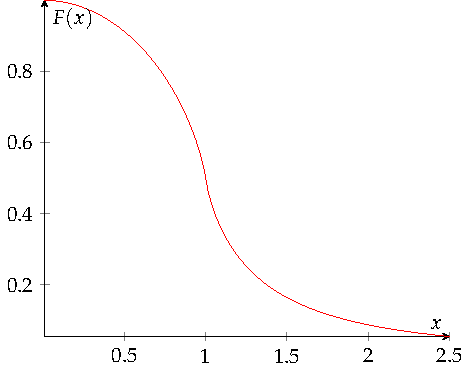
\includegraphics[]{Images/fig-Fplot.pdf}
    \caption{Plot of the function $F(x) = \frac{1}{2} + \frac{1-x^2}{4x}\ln\left|\frac{1 + x}{1-x}\right|$ which appears in the mean-field Hamiltonian dispersion relation. Note the divergence of $F'$ at $x = 1$ ($k = k_F$).}
    \label{fig-Fplot}
\end{figure}

We also recall the dispersion relation for free electrons:
\begin{align*}
    \e_0(\v{k}) = \frac{\hbar^2\v{k}^2}{2m}.
\end{align*}
We can plot the two dispersion relations side-by-side to compare them; this is done in Fig. \ref{fig-MFdispersionplot}.

\begin{figure}[htbp]
    \centering
    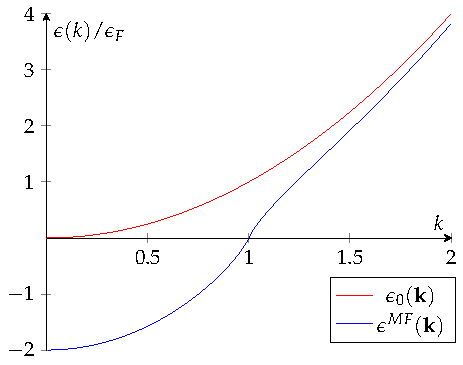
\includegraphics[]{Images/fig-MFdispersionplot.pdf}

    \caption{Plot of the free electron dispersion relation and the mean-field Hamiltonian dispersion relation. For the sake of plotting, we set $k_F =  1$.}
    \label{fig-MFdispersionplot}
\end{figure}

Note that at $k = k_F$, there is an unphysical divergence in $\nabla_\v{k}\e(\v{k})$. See HW1Q3 for more discussion of this problem, and how it can be remedied; namely, the source of the issue is the long-range Coulomb interaction. If we take into account screening, the problem goes away.

\subsection{Hartree-Fock as a Variational Bound}
Let us try to find the best possible $\e(\v{k})$ through the variational principle. We will look for $\e_0(\v{k}) + \eta_{\alpha\v{k}}$ with $\eta_{\alpha\v{k}}$ the variational parameter such that $\avg{H}_{MF}$ field is minimized. This expectation value is with respect to the ground state of the mean-field Hamiltonian.

This seems strange; we normally fix a Hamiltonian and then pick states over which we conduct an energy minimization. Here, the parameters appear in the mean-field Hamiltonian, but then the MF hamiltonian is sufficiently simple such that we know what the ground state is. So, the variational parameters directly determine the ground state of $H_{MF}$ which is the state we look at the expectation values for. Explicitly:
\begin{equation}
    \avg{H_0}_{MF} = \sum_{\v{k}\alpha}\e_0(\v{k})\avg{c^\dag_{\v{k}\alpha}c_{\v{k}\alpha}}_{MF} = \sum_{\v{k}\alpha}\e_0(\v{k})n_{\v{k}\alpha}
\end{equation}
\begin{equation}
    \begin{split}
        \avg{H_1}_{MF} &= \frac{1}{2}\sum_{\v{kpq}\alpha\beta}V(\v{q})\left[\avg{c^\dag_{\v{k} + \v{q}\alpha}c_{\v{k}\alpha}}_{MF}\avg{c^\dag_{\v{p} - \v{q}\beta}c_{\v{p}\beta}}_{MF} - \avg{c^\dag_{\v{k} + \v{q}\alpha}c_{\v{p}\beta}}_{MF}\avg{c^\dag_{\v{p} - \v{q}\beta}c_{\v{k}\alpha}}_{MF}\right]
        \\ &= \frac{1}{2}\sum_{\v{kpq}\alpha\beta}V(\v{q})\left[\delta_{\v{q} = 0}n_{\v{k}\alpha}n_{\v{p}\alpha} - \delta_{\v{k} + \v{q} = p}\delta_{\v{p} - \v{q} = \v{k}}\delta_{\alpha\beta}n_{\v{k}\alpha}n_{\v{p}\beta}\right]
        \\ &= \frac{1}{2}\left[V(0)\left(\sum_{\v{k}\alpha} n_{\v{k}\alpha}\right)^2 - \sum_{\v{k}\v{p}\alpha}V(\v{k} - \v{p})n_{\v{k}\alpha}n_{\v{p}\alpha}\right]
    \end{split}
\end{equation}
We get these pairings via the same ``destroy an electron in the Fermi sphere and then recover it'' argument we covered when discussing the second quantized form of the Jellium model. We now wish to minimize these expectation values w.r.t. our variational parameter $\eta$. One must remember that $\eta$ is implicitly hidden inside of the $n$s. We minimize via a chain rule:
\begin{equation}
        0 = \dpd{\avg{H}_{MF}}{\eta_{\v{q}\lambda}} = \sum_{\v{q}'\lambda'} \dpd{\avg{H}_{MF}}{n_{q'\lambda'}}\dpd{n_{q'\lambda'}}{{\eta_{\v{q}\lambda}}}
\end{equation}
and from this we obtain:
\begin{equation}\label{eq-lec512}
    \sum_{\v{k}\alpha}\left[e_0(\v{k}) + V(0)\sum_{\v{p}\beta}n_{\v{p}\beta} - \sum_{\v{p}}V(\v{k} - \v{p})n_{\v{p}\alpha}\right]\dpd{n_{q'\lambda'}}{{\eta_{\v{q}\lambda}}} = 0
\end{equation}
To solve this, consider:
\begin{equation}\label{eq-lec513}
    \dpd{\avg{H_{MF}}_{MF}}{\eta_{\v{q}\lambda}} = n_{\v{q}\lambda} + \sum_{\v{k}\alpha}\left[\e_0(\v{k}) + \eta_{\v{k}\alpha}\right]\dpd{n_{q'\lambda'}}{{\eta_{\v{q}\lambda}}}
\end{equation}
So substracting \eqref{eq-lec513} from \eqref{eq-lec512}, we obtain:
\begin{equation}
    \sum_{\v{k}\alpha}\left[-\eta_{\v{k}\alpha} + V(0)\sum_{\v{p}\beta}n_{\v{p}\beta} - \sum_{\v{p}}V(\v{k} - \v{p})n_{\v{p}\alpha}\right]\dpd{n_{\v{k}\alpha}}{\eta_{\v{q}\lambda}} = n_{\v{q}\lambda} -  \dpd{\avg{H_{MF}}_{MF}}{\eta_{\v{q}\lambda}}
\end{equation}
The solution is:
\begin{equation}
    \begin{split}
        \eta_{\v{k}\alpha} &= V(0)\sum_{\v{p}\beta}n_{\v{p}\beta} - \sum_{\v{p}}V(\v{k} - \v{p})n_{\v{p}\alpha}
        \\ n_{\v{q}\lambda} &= \dpd{\avg{H_{MF}}_{MF}}{\eta_{\v{q}\lambda}} = \avg{c^\dag_{\v{q}\lambda}c_{\v{q}\lambda}}_{MF}
    \end{split}
\end{equation}
It is easy to lose sight of what is being done through the many lines of writing, but one notices with the result that we have obtained the heuristic result using a very different method!

One way of justifying why the two approaches coincide; if we assume that the Hamiltonian takes the simple variational form, then the product of fluctuations that we have neglected in the heuristic approach exactly vanish; the operator approximation becomes exact.

We will not use this result immediately, but when we discuss tight-binding models and superconductivity, these approaches will be exceedingly useful.

Next time, we will discuss screening; when a test charge is put into an electron gas, there will be no long range interactions as the Coulomb force is screened by the cloud of electrons. Please by Wednesday read p.337-339 of A\&M; this is the ``Screening (General)'' section.
\newpage
\section{Screening}
\subsection{General Definitions and Setup of Problem}
For definitions and general discussion, see Ashcroft and Mermin p.337-339.

\begin{figure}[htbp]
    \centering
    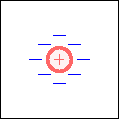
\includegraphics[]{Images/fig-screeningcartoon.pdf}
    \caption{Cartoon of electron screening; when a positive test charge is placed in a cloud of negative charge, the negative charges are attracted to the positive charge. This has the net effect of screening out the positive charge, as it gets neutralized to some capacity.}
    \label{fig-screeningcartoon}
\end{figure}
If we place a (positive) test charge in an cloud of negative charge, then it attracts negative charges around it, which results in a net screening of the positive charge. 

We have the potentials $\phi^{ext}, \phi$ and the charge densities $\rho^{ext}, \rho, \rho^{ind} = \rho - \rho^{ext}$. 

\begin{equation}\label{eq-potentialsdielectric}
    \begin{split}
        \phi(\v{q}) &= \frac{1}{\e(\v{q})}\phi^{ext}(\v{q})
        \\ \rho^{ind}(\v{q}) &= \chi(\v{q})\phi(\v{q})
        \\ \e(\v{q}) &= 1 - \frac{4\pi}{q^2}\chi(\v{q})
    \end{split}
\end{equation}
where $\e(\v{q})$ is the dielectric function and $\chi(\v{q})$ is the dielectric susceptibility. 

Today, we will go through two different calculations of the susceptibility.

\subsection{Thomas-Fermi Theory}
We have the second-quantized Hamiltonian:
\begin{equation}
    \begin{split}
        &\hat{H} = \int d^3x\hat{\psi}^\dag(\v{x})T(\v{x})\hat{\psi}(\v{x})
        \\ &T(\v{x}) = \frac{\hbar^2\nabla^2}{2m} - e\phi(\v{x})
    \end{split}
\end{equation}
we neglect $e-e$ interactions (including them makes this much more difficult). Of course electrons will see the total screened potential rather than the bare test charge potential, which this formula accounts for ($\phi$ vs. $\phi^{ext}$). 

For $\phi(\v{x}) = \phi_0$ a constant, we can solve the problem exactly. The Hamiltonian becomes:
\begin{equation}
    H = \sum_{\v{k}}\left(\frac{\hbar^2\v{k}^2}{2m} - e\phi_0\right)c_\v{k}^\dag c_\v{k} = \sum_{\v{k}}\e_\v{k}c_\v{k}^\dag c_\v{k}.
\end{equation}
Thomas-Fermi theory assumes that $\phi(\v{x})$ varies slowly on the scale $k_F^{-1}$; therefore in a semiclassical approximation, it is appropriate to write:
\begin{equation}
    \e_\v{k} \to \frac{\hbar^2\v{k}^2}{2m} - e\phi_0
\end{equation}
We will calculate the local electron density at $\v{r}$. It will be given by:
\begin{equation}\label{eq-screeningchargedensity}
    \begin{split}
        \rho(\v{r}) &= -e\avg{\hat{\psi}^\dag(\v{r})\hat{\psi}(\v{r})}
        \\ &= -2e\sum_{\v{k}\v{k}'}\avg{\hat{\psi}_{\v{k}}^\dag(\v{r})\hat{\psi}_{\v{k}'}(\v{r})c^\dag_{\v{k}}c_{\v{k}'}}
        \\ &= -2e\sum_{\v{k}\v{k}'}\hat{\psi}_{\v{k}}^\dag(\v{r})\hat{\psi}_{\v{k}'}(\v{r})\avg{c^\dag_{\v{k}}c_{\v{k}'}}
        \\ &= -2e\sum_{\v{k}\v{k}'}\hat{\psi}_{\v{k}}^\dag(\v{r})\hat{\psi}_{\v{k}'}(\v{r})\delta_{\v{k}\v{k}'}f(\e_{\v{k}}(\v{r}))
        \\ &= -2e\sum_{\v{k}}\abs{\psi_{\v{k}}(\v{r})}^2f(\e_{\v{k}}(\v{r}))
    \end{split}
\end{equation}
where the factor of $2$ comes from counting the two possible spin states, $f(\e_{\v{k}}(\v{r}))$ is the Fermi-Dirac distribution (which comes from the fact that at any temperature, the expectation value of the number of fermions of any state at a given energy is given from stat mech to be the FD distribution; previously we denoted this as $n_{\v{k}}$. For bosons next week it will be the BE-distribution), and in the last equality we use the Kronecker delta to perform the last of the summations. For the plane wave basis, we have $\psi_{\v{k}}(\v{r}) = \frac{1}{\sqrt{V}}e^{-i\v{k} \cdot \v{r}}$, so:
\begin{equation}
    \begin{split}
        \rho(\v{r}) &= -\frac{2e}{V}\sum_{\v{k}}\frac{1}{e^{\beta(\e_{\v{k}}(\v{r}) - \mu) + 1} + 1}
        \\ &= -en_0(\mu + e\phi(\v{r}))
    \end{split}
\end{equation}
where $\beta = \frac{1}{k_B T}$ as usual, and we define:
\begin{equation}
    n_0(\mu) = \int \frac{d^3k}{4\pi^3}\frac{1}{e^{\beta(\frac{\hbar^2\v{k}^2}{2m} - \mu) + 1} + 1}.
\end{equation}
We can now write the induced charge density as:
\begin{equation}\label{eq-rhoind}
    \rho^{ind}(\v{r}) = -e\left[n_0(\mu + e\phi(\v{r})) - n_0(\mu)\right] \approx -e^2\phi(\v{r})\dpd{n_0}{\mu}.
\end{equation}
which is just the difference between the total charge density and the average charge density in the sample (with no test charge), and we make the approximation that not only is $\phi$ slowly varying, but in itself small, allowing us to take the first-order Taylor approximation to $\rho^{ind}$ and neglect the higher-order terms.

Now, comparing Eqs. \eqref{eq-potentialsdielectric} and \eqref{eq-rhoind}, we can read off the dielectric susceptibility (and the function):
\begin{equation}\label{eq-TFresult}
    \boxed{\begin{split}
        \chi(\v{q}) &= -e^2\dpd{n_0}{\mu}
    \\ \e(\v{q}) &= 1 + \frac{4\pi e^2}{q^2}\dpd{n_0}{\mu}
    \end{split}}
\end{equation}
this is the main result of Thomas-Fermi theory of electron screening.

\subsection{Implications of Thomas-Fermi Theory}
Some housekeeping; Eq. \eqref{eq-TFresult} is often stated in the form:
\begin{equation}
    \e(\v{q}) = 1 + \frac{k_{TF}^2}{q^2}, \quad k_{TF} = 4\pi e^2\dpd{n_0}{\mu}.
\end{equation}
$k_{TF}$ is called the Thomas-Fermi momentum, and gives us a length scale for which the test charge is screened out. We illustrate the significance of $k_{TF}$ by considering the screened potential of a point charge:
\begin{equation}
    \phi^{ext}(\v{r}) = \frac{Q}{r} \to \phi^{ext}(\v{q}) = \frac{4\pi Q}{q^2}
\end{equation}
\begin{equation}
    \phi(\v{r}) = \frac{1}{\e(\v{q})}\phi^{ext}(\v{q}) = \frac{4\pi Q}{q^2 + k_{TF}^2}
\end{equation}
In real space, this becomes:
\begin{equation}
    \phi(\v{r}) = \int \frac{d^3}{(2\pi)^3}e^{i\v{q} \cdot \v{r}}\frac{4\pi Q}{q^2 + k_{TF}^2} = \frac{Q}{r}e^{-k_{TF}r}
\end{equation}
where the integral can be done by going into spherical coordinates. This is a very important result which tells us how screening acts in our simple Thomas-Fermi theory (though it is true more generally). This is known as the screened Coulomb, or Yukawa potential (often used in nuclear physics, though its origin is not electrostatic but nuclear). The presence of electrons exponentially supresses the test charge with distance, in particular the potential rapidly vanishes at distances $r > k_{TF}^{-1} = \lambda_{TF}$ which we call the screening length.

We may recall that we found a singularity in the derive in the effective dispersion when we covered Hartree-Fock theory. This was due to the long range interactions; but if one accounts for the screening/exponential suppression, then this singularity goes away.

As a last step, let us estimate the size of $\lambda_{TF}$ in a metal. We have that:
\begin{equation}
    \dpd{n_0}{\mu} = -\int \frac{d^3k}{4\pi^3}\dpd{}{\mu}\left[\frac{1}{e^{\beta(\e_\v{k} - \mu)} + 1}\right] \longrightarrow^{T \to 0} \int \frac{d^3k}{4\pi^3}\delta(\e_{\v{k}} - \mu) = g(\mu) = \frac{mk_F}{\hbar^2 \pi^2}
\end{equation}
where the last quantity is just the density of states at the Fermi level in 3-D. Sticking this into the result for $k_{TF}$, we get:
\begin{equation}
    \frac{k_{TF}^2}{k_F^2} = \frac{4}{\pi}\frac{me^2}{\hbar^2k_F} = \frac{4}{\pi} \frac{1}{a_0k_F} = \left(\frac{16}{3\pi^2}\right)^{3/2}r_s \implies k_{TF} = 0.815k_F\sqrt{r_s} \implies \lambda_{TF} \approx k_{F}^{-1} = \frac{\sqrt{r_s}}{2.95}A^{\circ}
\end{equation}
This tells us that in a metal (where $r_s = 2-6$), the Coulomb interaction is screened at very short distances, comparable to the ionic spacings.

A comment: We have made the semiclassical assumption that $\phi$ varies slowly; but it does not vary slowly on the given length scale. It's not valid in real materials, but it is still a useful result. 

\subsection{Lindhard Theory}
In the Lindhard theory, we assume that $\phi(\v{r})$ is small and can be treated as a perturbation:
\begin{equation}
    H = \frac{\hbar^2 \nabla^2}{2m} - e\phi(\v{r})
\end{equation}
where the first term is $H_0$ and the second is $H_1$. This approximation is almost always valid. We calculate the charge density using Eq. \eqref{eq-screeningchargedensity}. We will need to find the correction to $\psi_{\v{k}}(\v{r})$ due to perturbation. This correction looks like:
\begin{equation}
    \psi_{\v{k}}(\v{r}) = \psi_{\v{k}}^0(\v{r}) + \sum_{\v{k}'}\frac{\bra{\psi^0_{\v{k}'}}-e\phi(\v{r})\ket{\psi^0_{\v{k}'}}}{\e_{\v{k}} - \e_{\v{k}'}}\psi_{\v{k}'}^0(\v{r}) + \ldots
\end{equation}
Now, since:
\begin{align*}
    \psi_{\v{k}}^0(\v{r}) = \frac{1}{\sqrt{V}}e^{i\v{k} \cdot \v{r}}, \quad \e^0_{\v{k}} = \frac{\hbar^2\v{k}^2}{2m}
\end{align*}
we have:
\begin{equation}
    \bra{\psi_\v{k}'^0}-e\phi(\v{r})\ket{\psi_{\v{k}}^0} = -\frac{e}{V}\int d^3r e^{-i\v{k}' \cdot \v{r}} \phi(\v{r})e^{i\v{k} \cdot \v{r}} = -\frac{e}{V}\phi(\v{k} - \v{k}')
\end{equation}
where in the last equality we recognize the operation being carried out as a Fourier transform. We now have:
\begin{equation}
    \psi_\v{k}(\v{r}) = \psi_{\v{k}}^0(\v{r}) - \frac{e}{V}\sum_{\v{k}'}\frac{\phi(\v{k} - \v{k'})}{\e^0_{\v{k}} - \e^0_{\v{k}'}}\psi^0_{\v{k}'}(\v{r})
\end{equation}
We then substitute $\psi_\v{k}(r)$ into Eq. \eqref{eq-screeningchargedensity} and retain terms up to first order in $\phi(\v{k} - \v{k}')$. This yields:

\begin{equation}
    \rho(\v{r}) = -e\left[\sum_{\v{k}}f_k\abs{\psi_\v{k}^0}^2 - \frac{e}{V}\sum_\v{k}\left(f_\v{k}\psi_\v{k}^{0*}\sum_{\v{k}'} \frac{\psi^0_{\v{k}'}}{\e^0_\v{k} - \e^0_{\v{k}'}}\phi(\v{k} - \v{k}') + c.c.\right)\right]
\end{equation}

Where the first term is $\rho_0(\v{r})$ and the second term is $\rho^{ind}(\v{r})$. $f_\v{k}$ is the Fermi-dirac distribution for energy $\e_{\v{k}}$. We can evaluate this integral using the substitution:
\begin{align*}
    (\v{k}, \v{k}') \to (\v{k} + \frac{1}{2}\v{q}, \v{k} - \frac{1}{2}\v{q})
\end{align*}
We then obtan:
\begin{equation}
    \rho^{ind}(\v{r}) = -\frac{e^2}{V}\sum_{\v{q}}e^{i\v{q} \cdot \v{r}}\left(\sum_{\v{k}} \frac{f_{\v{k} + \frac{1}{2}\v{q}} - f_{\v{k} - \frac{1}{2}\v{q}}}{\e^0_{\v{k} + \frac{1}{2}\v{q}} - \e^0_{\v{k} - \frac{1}{2}\v{q}}}\right) \phi(\v{q})
\end{equation}
we can therefore conclude that $\rho^{ind}(\v{q}) = \chi(\v{q})\phi(\v{q})$, where:
\begin{equation}
    \boxed{\chi(\v{q}) = -\frac{e^2}{V}\sum_{\v{k}} \frac{f_{\v{k} + \frac{1}{2}\v{q}} - f_{\v{k} - \frac{1}{2}\v{q}}}{\e^0_{\v{k} + \frac{1}{2}\v{q}} - \e^0_{\v{k} - \frac{1}{2}\v{q}}}}
\end{equation}
This is our final result, the Lindhard susceptibility function. WE note that $\chi(\v{q})$ looks different from the Thomas-Fermi case, and there is an explicit dependence of $\chi(\v{q})$ on $\v{q}$. 

\subsection{Limits of the Lindhard Results}
We look at two limits. At low $T$ and small $q$, the numerator is small unless $\abs{\v{k}} \approx k_F$ (we subtract two near-step functions in the numerator, and the difference is only nonzero for $\abs{\v{k}} \approx k_F$). Therefore we can expand:
\begin{equation}
    f_{\v{k} \pm \frac{1}{2}\v{q}} \approx f_\v{k} \pm \frac{\hbar^2}{2}\frac{\v{k} \cdot \v{q}}{m}\dpd{f_\v{k}}{\mu} + O(q^2)
\end{equation}
so we get:
\begin{equation}
    \chi(\v{q}) \approx -\frac{e^2}{V}\sum_{\v{k}}\dpd{f_\v{k}}{\mu}
\end{equation}
we recover the TF result! This makes sense, as the small $q$ limit is the large-wavelength limit, i.e. $\phi$ varies slowly.

At $T = 0$, the $\v{k}$ integral can be evaluated exactly:
\begin{equation}
    \chi(\v{q}) = -e^2\left(\frac{mk_F}{\pi^2\hbar^2}\right)\left[\frac{1}{2} + \frac{1-x^2}{4x^2}\ln\left|\frac{1+x}{1-x}\right|\right]
\end{equation}
where $x = q/2k_F$. This is the same function that appeared in our discussion of Hartree-Fock, and it is non-analytic at $x = 1$. Because the dielectric function $\e(\v{q}) = 1 - \frac{4\pi}{q^2}\chi(\v{q})$ is non-analytic at $q \to 2k_F$, it is possible to show that the screened potential of a point charge contains a term:
\begin{equation}
    \phi(\v{r}) \approx \frac{1}{r^3}\cos(2k_F r)
\end{equation}
for $r \gg k_F^{-1}$. This is known as the ``Friedel'', or ``RKKY'' oscillation (so to recap, we have an exponetially decaying term, and we also have a power-law decaying oscillatory term). It is observable experimentally, using STM.

Why is this? Electrons come in to screen the test charge, but ``overscreen'', creating a region of high negative charge density. So then the electrons go away from this region to compensate, and this leads to this oscillatory effect.

Next class, we study bosonic excitations in solds.
\newpage
\section{Bosons, Bose-Einstein Condensation, and Helium-4}
\subsection{Housekeeping}
Reading assignment: Fermi liquid theory in Aschroft and Mermin p345-357. We don't have quite the mathematical tools to explain it, but the excerpt above gives a short qualitative introduction.

Midterm and Final: MT on First week of November. Both exams have the same structure; short in class portion (10-15 minutes), questions concerning things we are expected to know (e.g. $r_s = 2-6$ in metals, or temperature resistivity in Fermi liquid theory is $T^2$ etc.). Then there is a takehome portion with homework-level questions.

\subsection{Boson types and statistics}

But now we switch gears from fermions to bosons. There are two types of bosonic particles we consider in our discussion:
\begin{enumerate}[(a)]
    \item ``Real'' (number-conserving): $\phantom{i}^4\text{He}, \text{Rb}, \text{Na}, \text{K}, \ldots$
    \item ``Emergent'': Phonons (quanta of lattice vibrations), Magnons, \ldots 
\end{enumerate}
The main difference is that for the first class, the number of particles is conserved; the number of Helium atoms in a closed container is fixed. On the other hand, phonons can be created and destroyed out of thin air, so to speak. So there is no conservation law for them.

An important distinction between bosons and fermions is the type of statistics they obey. Mathematically, this is based on commutation relations; in terms of second quantization, bosons obey the commutation relations:
\begin{equation}
    \begin{split}
        &[a_\v{k}^\dag, a_\v{k'}] = \delta_{\v{k}\v{k}'}
        \\ &[a_\v{k}^\dag, a_\v{k'}^\dag] = [a_\v{k}, a_\v{k'}] = 0.
    \end{split}
\end{equation}
Recall the Pauli exclusion principle for fermions (which could be derived from the anticommutation relations); no such principle exists for bosons, of which any number are free to occupy the same quantum state. These commutation relations give rise to the BE distribution function:
\begin{align*}
    \bar{n}_\v{k} = \frac{1}{e^{\beta(\e_{\v{k}} - \mu)} - 1}
\end{align*}
where compared to the FD distribution, the sign in the denominator has flipped. 

\subsection{Deriving the Bose-Einstein Distribution}
Let's review how this distribution function comes about. Consider a non-interacting system:
\begin{equation}
    H = \sum_{\v{k}}(\e_{\v{k}} - \mu)a^\dag_{\v{k}}a_\v{k}
\end{equation}
The thermal average of any operator $\hat{O}$ is given by:
\begin{equation}
    \begin{split}
        \avg{\hat{O}}_\beta &= \frac{1}{Z}\sum_j \bra{j}\hat{O}\ket{j}e^{-\beta (E_j - \mu N)}
    \\  Z &= \sum_j e^{-\beta (E_j - \mu N)}.
    \end{split}
\end{equation}
where the matrix elements of $\hat{O}$ are weighted by the boltzmann factor, of which the partition function $Z$ is the sum of:
Note we use the grand canonic ensemble so we have the $\mu N$. We then have:
\begin{equation}
    \begin{split}
        \avg{\hat{n}_\v{k}} &= \frac{1}{Z}\sum_j \bra{j}a^\dag_{\v{k}}a_{\v{k}}e^{-\beta(\hat{H} - \mu\hat{N})}\ket{j}
        \\ &= \frac{1}{Z}\Tr(a_\v{k}^\dag a_\v{k} e^{-\beta(\hat{H} - \mu\hat{N})})
        \\ &= \frac{1}{Z}\Tr(a_\v{k} e^{-\beta(\hat{H} - \mu\hat{N})}a_\v{k}^\dag)
        \\ &= \frac{1}{Z}\Tr(a_\v{k} a_\v{k}^\dag e^{-\beta(\hat{H} - \mu\hat{N})}e^{-\beta(\e_{\v{k}} - \mu)})
        \\ &= \frac{1}{Z}\Tr((1 + a_\v{k}^\dag a_\v{k}) e^{-\beta(\hat{H} - \mu\hat{N})}e^{-\beta(\e_{\v{k}} - \mu)})
        \\ &= (1 + \avg{\hat{n}_\v{k}})e^{-\beta(\e_{\v{k}} - \mu)}
    \end{split}
\end{equation}
where in the first line, we take advantage of the fact that when $\hat{H}$ acts on its eigenstate, it gives back the eigenvalue. So we can pull the constant into the matrix element and convert the energy into the Hamiltonian. The second line we cast this expression as a trace. In the third line we use the cyclicity of the trace. In the fourth line we skip some math (but it can be done in detail) but this can be viewed as creating a single boson with energy $\e_{\v{k}}$. In the fifth line we use the bosonic commutation relations. In the sixth line we evaluate the expression. We can then solve for $\avg{\hat{n}_\v{k}}$ to obtain:
\begin{equation}
    \avg{\hat{n}_\v{k}} = \frac{1}{e^{\beta(\e_{\v{k}} - \mu)} - 1}.
\end{equation}
Note that a similar derivation can be done for Fermions to get the Fermi-Dirac distribution.

\subsection{Bose-Einstein Condensation}
BE Condensation occurs in real (or number conserving) bosons, most famously Helium-4 at low temperature. The easiest way to see this occurs is to consider the total number of bosons $N$:
\begin{equation}
    N = \sum_\v{k}\bar{n}_\v{k} = \sum_{\v{k}}  \frac{1}{e^{\beta(\e_{\v{k}} - \mu)} - 1}, \quad \e_{\v{k}} = \frac{\hbar^2\v{k}^2}{2m}
\end{equation}
Note that for real bosons $\mu \leq 0$; otherwise we would have $\bar{n}_{\v{k}} < 0$ for some $\v{k}$ which is forbidden. This implies that:
\begin{align*}
    e^{\beta(\e_{\v{k}} - \mu)} \geq e^{\beta\e_{\v{k}}}
\end{align*}
For this reason, we can bound the total number of bosons from above:
\begin{equation}
    \begin{split}
        N &\leq \sum_{\v{k}}\frac{1}{e^{\beta \e_{\v{k}}} - 1}
        \\ &= N_0 + \frac{\Omega}{(2\pi)^3}\int_0^\infty dk \frac{4\pi k^2}{e^{\beta\hbar^2k^2/2m} - 1}
    \end{split}
\end{equation}
where we have separated the sum into two terms; the $\v{k} = 0$ term (which is problematic as it formally diverges; it only comes about as we have discarded the chemical potential) and the rest of the sum rewritten as an integral, which we call $N'(T)$. $\Omega$ here is the volume. We leave the $N_0$ term for now and evaluate the $N'(T)$ by substitution. We let $x = \beta\frac{\hbar^2k^2}{2m}$ and $dx = \beta\frac{\hbar^2}{m}kdk$ so:
\begin{equation}
    N'(T) = \frac{\Omega}{(2\pi)^3}4\pi \sqrt{2}\left(\frac{m}{\beta\hbar^2}\right)^{3/2}\int_{0^+}^\infty \frac{\sqrt{x}dx}{e^x - 1} = C\Omega T^{3/2}
\end{equation}
The actual integral on the right is a finite constant (formally it can be evaluated by considering the Riemann zeta function), but we are really only interested in the temperature dependence, so we've lumped things into a constant $C$. It's also important that $N'(T)$ is extensive/grows proportionally to the system volume. Now we look at how BE condensation comes about from this. We rewrite the inequality as:
\begin{align*}
    N \leq N_0 + N'(T)
\end{align*}
We plot $N'(T)$ as a function of $T$. $N$ is fixed. There is some $T_c$ for which $N'(T)$ intersects $N$; above $T_C$, we have $N_0 = 0$, and below $T_c$ we have $N_0 > 0$. We have an extensive number of bosons in the $\v{k} = \v{0}$ state. This is what is known as BE condensation. In particular as we take $T \to 0$ all of the bosons occupy the ground state. This is not surprising; in the view of QM, if we try to minimize the energy of a set of bosons, we can just cram them all into the ground state (there is nothing preventing us from doing this; no Pauli exclusion)! However in terms of classical physics this phenomena was unusual.

\begin{figure}[htbp]
    \centering
    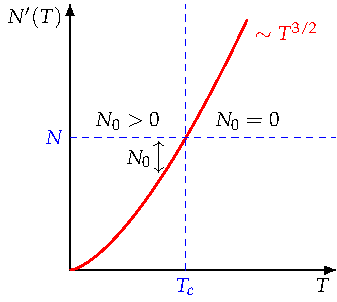
\includegraphics[]{Images/fig-superfluidN.pdf}
    \caption{Plot of the upper bound of excitated state bosons $N'(T)$ as a function of temperature $T$. Above some $T_c$, we have zero bosons in the ground state and so $N_0 = 0$. Below some $T_c$, we have that $N_0 > 0$ and so an extensive number of bosons occupy the $\v{k} = 0$ ground state; we therefore have Bose-Einstein condensation.}
    \label{fig-superfluidN}
\end{figure}

\subsection{Bogoliubov Theory of Helium-4}
This is a classic theory; 1946 (but still valid to this day)! Helium-4 was interesting from the early days of physics at it had interesting superfluid properties. Bogoliubov started off this explanation, and Landau later would give an argument for why Helium-4 is superfluidic (which we cover next lecture).

We consider weakly interacting (spinless) bosons described by the Hamiltonian:
\begin{equation}
    H = \sum_{\v{k}} \e_{\v{k}}a^{\dag}_{\v{k}}a_\v{k} + \frac{1}{2}\sum_{\v{k}\v{p}\v{q}}V_{\v{q}}a^\dag_{\v{k} - \v{q}}a^{\dag}_{\v{p} + \v{q}}a_\v{p}a_\v{k}
\end{equation}
where $V_\v{q}$ is a Fourier transform of a short-range interatomic potential; it is a short range interaction that dies off quickly outside of the Helium atom (on the order of an Angstrom). As usual, $\e_{\v{k}} = \frac{\hbar^2\v{k}^2}{2m}$. We assume (following Bogoliubov) that $V_{\v{q}}$ is weak and $T \ll T_c$. Then we expect the ground state to be close to a perfect BEC, where:
\begin{equation}
    \ket{\Phi^N_0} = (a^\dag_\v{0})^N\ket{0}
\end{equation}
Now we perform the following approximation:
\begin{equation}\label{eq-Napproxbogo}
    \begin{split}
        &a^\dag_\v{0}a_\v{0} \to \avg{a^\dag_\v{0}a_\v{0}} = N_0 \approx N
        \\&a^\dag_\v{0}a^\dag_\v{0} \to N_0
    \end{split}
\end{equation}
The first line: whenever we see the number operator, we take it to be its average value, which is large/close to the total number. The second line is less obvious, but consider $a_\v{0}^\dag a_{\v{0}}^\dag \ket{\Phi_0^N} = \sqrt{(N_0 + 1)(N_0 + 2)}\ket{\Phi_0^{N+2}}$ and we can then take $\sqrt{(N_0 + 1)(N_0 + 2)} \approx N_0$ for $N_0$ large. The assumption being made is that the Hamiltonian is always acting on a state close to the perfect BEC ground state, so we can approximate these operators as we have above. In the interaction term, we split all sums as:
\begin{align*}
    \sum_{\v{k}} = \sum_{\v{k} = 0} + \sum_{\v{k}}'
\end{align*}
and retain only terms containing at least only one power of $N_0$. This is a bit of a mess (as we have 8 sums to work with... ); we will not go through it explicitly, but we justify this approximation by saying that since $N_0$ is large, all terms without powers of $N_0$ are relatively small and hence can be neglected. The result is as follows:
\begin{equation}
    H \approx \sum_{\v{k}}\e_{\v{k}}a^\dag_\v{k}a_\v{k} + \frac{1}{2}N_0^2 V_0 + N_0V_0\sum_{\v{k}}' a_\v{k}^\dag a_\v{k} + N_0\sum_\v{q}'V_\v{q}a^\dag_{\v{q}}a_\v{q} + \frac{1}{2}N_0\sum_\v{q}' V_\v{q}(a_\v{q}a_{-\v{q}} + a_\v{q}^\dag a_{-\v{q}}^\dag)
\end{equation}
The first (kinetic energy) term remains unchanged. The second term comes from $\v{k} = v{q} = \v{p} = \v{0}$, The third term comes from $\v{p} = \v{q} = \v{0}$ or $\v{k} = \v{q} = \v{0}$ and so on. To simplify, we define:
\begin{equation}
    \begin{split}
        \eta_\v{k} &= N_0V_\v{k}
        \\ \hbar \Omega_\v{k} &= \e_\v{k} + \eta_\v{k}.
    \end{split}
\end{equation}
Notice also that $N_0 + \sum_\v{k}' a^\dag_\v{k}a_\v{k} \approx N$. where $N_0, N \gg N' = \sum_\v{k}' a^\dag_\v{k}a_\v{k}$. With this, let us combine some terms:
\begin{equation}
    \frac{1}{2}N^2V_0 = \frac{1}{2}V_0\left[N_0^2 + 2N_0\sum_\v{k}' a^\dag_\v{k}a_\v{k} + \ldots \right]
\end{equation}
Hence we can write the entire Hamiltonian as:
\begin{equation}\label{eq-He4aHamiltonian}
    H \approx \frac{1}{2}N^2 V_0 + \sum_{\v{k}}\left[\hbar \Omega_\v{k}a^\dag_\v{k}a_\v{k} + \frac{1}{2}\eta_\v{k}(a_\v{k}a_{-\v{k}} + a^\dag_\v{k}a^\dag_{-\v{k}})\right]
\end{equation}
We draw our attention to the last term(s); these are ``anomalous terms'', which \emph{do not} conserve particle number. This is a consequence of the Bogoliubov approximation. Physically, $a_\v{k}a_{-\v{k}}$ represent bosons $(\v{k}, -\v{k})$ ``disappearing'' into the condensate. The number of bosons in the condensate is so large that you do not have to keep track of the bosons in the condensate itself; we only need to keep track of the other particles as they disappear and appear out of it.

\subsection{Bogoliubov Transformations and Quasiparticle Spectrum}
Bogoliubov also developed a theory of how to treat such Hamiltonians. They can be diagonalized by means of Bogoliubov transformations:
\begin{equation}
    \begin{split}
        a_\v{k} &= \mu_\v{k}\alpha_\v{k} + \nu_\v{k}\alpha^\dag_{-\v{k}} \vert \alpha_\v{k} = \mu_{\v{k}}a_\v{k} - \nu_\v{k}a^\dag_{-\v{k}}
        \\ a_\v{k}^\dag &= \mu_\v{k}\alpha_\v{k}^\dag + \nu_\v{k}\alpha_{-\v{k}} \vert \alpha_\v{k}^\dag = \mu_{\v{k}}a^\dag_\v{k} - \nu_\v{k}a_{-\v{k}}
    \end{split}
\end{equation}
where we have the forwards transformations on the left and the inverse transformation on the right. Here, $\alpha_\v{k}$ are our new bosonic ``quasiparticle'' operators and $(\mu_\v{k}, \nu_\v{k})$ are real coefficients. We want this to be a canonical transformation, so we want these new $\alpha$ operators to satisfy the same commutation relations as the $a$s. This is important as it will place constraints on the $\mu_\v{k}$ and $\nu_{\v{k}}$. Let's see what happens:
\begin{equation}
    \begin{split}
        [\alpha_\v{k}, \alpha^\dag_{\v{k}'}] &= [\mu_{\v{k}}a_\v{k} - \nu_\v{k}a^\dag_{-\v{k}}, \mu_{\v{k}'}a^\dag_{\v{k}'} - \nu_{\v{k}'}a_{-\v{k}'}]
    \\ &= \mu_{\v{k}}\mu_{\v{k}'}[a_\v{k}, a^\dag_{\v{k}'}] + \nu_{\v{k}}\nu_{\v{k}'}[a^\dag_{-\v{k}}, a_{-\v{k}'}]
    \\ &= (\mu_{\v{k}}^2 - \nu_{\v{k}}^2)\delta_{\v{k}\v{k}'}
    \end{split}
\end{equation}
where we have used the known commutation relations for the $a$s. So we obtain the constraint:
\begin{equation}
    [\alpha_\v{k}, \alpha^\dag_{\v{k}'}] = \mu_{\v{k}}^2 - \nu_{\v{k}}^2 = 1.
\end{equation}

A comment: we want to find $(\mu_\v{k}, \nu_\v{k})$ such that the resulting $H$ is diagonal, that is:
\begin{equation}
    H = \sum_{\v{k}}\hbar \omega_\v{k}\alpha^\dag_{\v{k}}\alpha_\v{k} + E_0.
\end{equation}
So to this end we compute:
\begin{equation}
    \begin{split}
        \alpha^\dag_{\v{k}}\alpha_\v{k} &= (\mu_{\v{k}}a^\dag_\v{k} - \nu_\v{k}a_{-\v{k}})(\mu_{\v{k}}a_\v{k} - \nu_\v{k}a^\dag_{-\v{k}})
        \\ &= \mu_\v{k}^2a^\dag_\v{k}a_\v{k} + v_k^2a_{-\v{k}}a^\dag_{-\v{k}} - \mu_\v{k}\nu_{\v{k}}(a_\v{k}a_{-\v{k}} + a^\dag_{\v{k}}a^\dag_{-\v{k}})
    \end{split}
\end{equation}
Comparing this with the form of the Hamiltonian, we can see we are on the right track. The only terms to seem to not appear there are the $a_{-\v{k}}a^\dag_{-\v{k}}$s but we recognize the sum to run over all $\v{k}$ and so we can make a substitution there. We make an assumption that $\omega_\v{k} = \omega_{-\v{k}}$ and $\nu_{\v{k}}^2 = \nu_{-\v{k}}^2$ (we can check later that this is consistent) then:
\begin{equation}
    \sum_{\v{k}}\hbar \omega_{\v{k}}\alpha^\dag_{\v{k}}\alpha_{\v{k}} =  \sum_{\v{k}}\hbar \omega_{\v{k}}(\mu_{\v{k}}^2 + \nu_{\v{k}}^2)a^\dag_\v{k}a_\v{k} + \sum_{\v{k}}\hbar \omega_\v{k}\nu_{\v{k}}^2 - \sum_{\v{k}}\hbar \omega_{\v{k}}\mu_{\v{k}}\nu_{\v{k}}(a_\v{k}a_{-\v{k}} + a^\dag_{\v{k}}a^\dag_{-\v{k}})
\end{equation}
Comparison with the original Hamiltonian (Eq. \eqref{eq-He4aHamiltonian}) implies:
\begin{equation}
    \begin{split}
        \hbar \omega_\v{k}(\mu_{\v{k}}^2 + \nu_\v{k}^2) &= \hbar \Omega_{\v{k}}
    \\ 2\hbar \omega_{\v{k}}\mu_{\v{k}}\nu_{\v{k}} &= \eta_{\v{k}}
    \end{split}
\end{equation}
To solve for $\omega_{\v{k}}$ we square both equations and subtract:
\begin{align*}
    (\hbar \omega_{\v{k}})^2\left[(\mu_{\v{k}}^2 + \nu_{\v{k}}^2)^2 - 4\mu_{\v{k}}^2\nu_{\v{k}}^2\right] = (\hbar\Omega_{\v{k}})^2 - \eta_{\v{k}}^2
\end{align*}
but on the RHS We have $(\mu_{\v{k}} - \nu_{\v{k}})^2 = 1$ and so the dependence on $\mu/\nu$ drops out and we have:
\begin{equation}
    \hbar\omega_{\v{k}} = \sqrt{\hbar^2\Omega_{\v{k}}^2 - \eta_\v{k}^2} = \sqrt{\e_{\v{k}}(\eta_\v{k} + 2NV_\v{k})}
\end{equation}
which is one of the main results of Bogoliubov theory, the ``spectrum of quasiparticle excitations''. This spectrum will have interesting implications; among other things, it will be the basis for superfluidity in liquid He-4 according to the Landau argument. Let us discuss some special cases of this spectrum. 

\subsection{Quasiparticle Spectrum - Special Cases}
\subsubsection{Non-Interacting}
If the bosons are noninteracting, then $V_{\v{k}} = 0$ and so:
\begin{align*}
    \hbar\omega_{\v{k}} = \sqrt{\e_{\v{k}}^2} = \frac{\hbar^2\v{k}^2}{2m}
\end{align*}
so we indeed reproduce our prior result for free bosons.

\subsubsection{Contact Repulsion}
We take $V(\v{r}) = U\delta(\v{r})$ (i.e. the bosons repel when they are on top of each other). Since the FT of a dirac delta is just a constant, we have:
\begin{align*}
    V_{\v{k}} = \frac{U}{\Omega}
\end{align*}
for all $\v{k}$. We then have:
\begin{equation}
    \hbar\omega_\v{k} = \sqrt{\e_\v{k}(\e_\v{k} + 2(NU/\Omega))} = \begin{cases}
        \sqrt{\e_\v{k}E_0} \sim \abs{\v{k}}, \quad \e_{\v{k}} \ll E_0 \text{ (long wavelength = sound-like dispersion)}
        \\ \abs{\e_\v{k}} \sim \v{k}^2, \quad \e_{\v{k}} \gg E_0 \text{ (short wavelength = particle-like dispersion)}
    \end{cases}
\end{equation}
where we define $2(NU/\Omega) = E_0$. So the weak interactions of Helium modify the dispersion from particle like to sound-like at long wavelengths with linear dispersion relation.

\subsubsection{Typical Helium-4 Interaction}
The Fermi velocity scales as:
\begin{figure}[htbp]
    \centering
    \textcolor{blue}{$v_k$ vs. $\v{k}$.}
    \caption{<caption>}
    \label{<label>}
\end{figure}
From this we obtain a dispersion relation that looks as follows:
\begin{figure}[htbp]
    \centering
    \textcolor{blue}{dispersion relation}
    \caption{<caption>}
    \label{<label>}
\end{figure}

This concludes the Bogoliubov theory of Helium-4 in a nutshell. In the next assignment we will explicitly calculate the coefficients in the Bogoliubov transformation and other fun exercises.

\subsection{Landau Argument for Superfluidity}
To conclude, we cover Landau's argument for superfluidity for Liquid Helium 4. At the time, it was a known experimental fact that liquid Helium-4 would flow in a tube without friction. Experiments were also done where one would start spinning a bucket of Helium-4 at temperature above $T_c$, then the friction would cause it to rotate; then if one cooled the bucket down, the Helium would continue to rotate indefinitely.

Landau considered the following scenario. He considered a vessel of liquid Helium-4 and an object of large mass $M \gg m$ moving with velocity $\v{v}$. The question Landau asked was can the object relax its energy and momentum by emitting quasiparticle excitations? 

\begin{figure}[htbp]
    \centering
    \textcolor{blue}{TODO- cartoon figure}
    \caption{<caption>}
    \label{<label>}
\end{figure}

We will show that it is impossible to conserve both energy and momentum and for the particle to relax so long as the object does not exceed a critical velocity $v_c$. Energy conservation and momentum conservation tell us that:
\begin{equation}
    \begin{split}
        \frac{1}{2}M\v{v}^2 &= \frac{1}{2}M\v{v}'^2 + \hbar \omega_{\v{k}}
        \\ M\v{v} &= M\v{v}' + \hbar\v{k}
    \end{split}
\end{equation}
These are the two equations we must satisfy if this process is allowed.
Squaring the second equation, we have:
\begin{align*}
    M^2\v{v}'^2 = M^2\v{v}^2 + \hbar^2\v{k}^2 - 2M\hbar \v{k} \cdot \v{v}
\end{align*}
We can divide out by $2M$ and combine the two conservation equations to find:
\begin{equation}
    \hbar \v{v} \cdot \v{k} = \frac{\hbar^2\v{k}^2}{2M} + \hbar \omega_\v{k}
\end{equation}
We consider $M \gg m$. and so we can neglect the $ \frac{\hbar^2\v{k}^2}{2m}$ term. Further we can let $\v{v} \cdot \v{k} = \abs{\v{v}}\abs{\v{k}}\cos\theta$ and so:
\begin{equation}
    \hbar \abs{\v{v}}\abs{\v{k}}\cos\theta = \hbar \omega_\v{k}
\end{equation}
For low enough velocities, the LHS will always be less than the RHS.

\begin{figure}[htbp]
    \centering
    \textcolor{blue}{TODO- roton curve with bound}
    \caption{<caption>}
    \label{<label>}
\end{figure}

The graphical solution shows that slow moving objects cannot dissipate energy and momentum in liquid Helium-4. We therefore have dissipationless motion, or superflow.

Note that one can solve for a critical velocity:

\begin{equation}
    v_c = \min_\v{k}\left(\frac{\omega_\v{k}}{\abs{\v{k}}}\right) \approx 1\si{cm.s^{-1}} \text{ in Helium-4}
\end{equation}

Note that the actual critical velocity is 10 times slower, due to neglected effects such as the creation of vortex rings etc. but nevertheless Landau's argument is an argument that provides some nice explanatory power!

Question: Why does argument not predict superfluid flow in general life situations? This is left as an exercise for the reader\dots


\newpage
\section{Lattice Vibrations \& Phonons}
\subsection{Phonons in One Dimension}
We consider a simple monoatomic chain:
\begin{figure}[htbp]
    \centering
    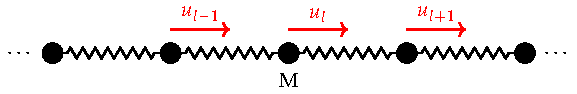
\includegraphics[]{Images/fig-monochaincartoon.pdf}

    \caption{A monoatomic chain. The atoms are of mass $M$ and are labelled with index $l$, with $u_l$ denoting the $l$th-atoms' displacement from equilibrium.}
    \label{fig-monochaincartoon}
\end{figure}
We label the atoms by index $l$ and the displacements from equilibrium for the $l$th atom by $u_l$. We assume we have a crystal lattice with individual atoms oscillating around equilibrium positions. The general Hamiltonian we can write for this system is:
\begin{equation}
    \begin{split}
        &H = \sum_l \frac{p_l^2}{2M} + V(u_1, u_2, \ldots)
        \\ &p_l = -i\hbar\dpd{}{u_l}
        \\ &[u_l, p_{l'}] = i\hbar\delta{ll'} 
    \end{split}
\end{equation}
Where we take the momentum to be canonically conjugate to the displacement and hence it satisfies the canonical commutation relation. We assume that the potential has a minimum for $u_l = 0$ for all $l$. We expand $V$ in a Taylor series about these minima:
\begin{equation}\label{eq-Vtaylor}
    V(u_1, u_2, \ldots) = V(0, 0, \ldots ) + \sum_l u_l \left[\dpd{V}{u_l}\right]_{u_1=u_2=\ldots = 0} + \frac{1}{2!}\sum_{l, l'}u_lu_{l'}\left[\frac{\partial^2 V}{\partial \mu_l \partial \mu_{l'}}\right]_{u_1=u_2=\ldots=0} + \frac{1}{3!} \ldots
\end{equation}
The first term can be eliminated by suitable choice of energy zero (a constant in the Hamiltonian changes none of the physics). The second term vanishes by virtue of $u_1 = u_2 = \ldots = 0$ being a minimum of $V$. We are left with just the second-order term, and so:
\begin{equation}
    H \approx \sum_l \frac{p_l^2}{2M} + \frac{1}{2}\sum_{l, l'}u_l V_{ll'}u_{l'}
\end{equation}
where $V_{ll'} = \left[\frac{\partial^2 V}{\partial \mu_l \partial \mu_{l'}}\right]_{u_1=u_2=\ldots=0}$ is the dynamical matrix. We neglect all higher order terms in Eq. \eqref{eq-Vtaylor} which amounts to a harmonic approximation.

\subsection{Diagonalizing the Potential}

We next diagonalize the $V$-term. To this end, we define a vector of displacements:
\begin{align*}
    Y = \m{\mu_1 \\ \mu_2 \\ \vdots \\}
\end{align*}
and then we have:
\begin{align*}
    V = \m{V_{11} & V_{12} & \ldots
    \\ V_{21} & \ddots & 
    \\ \vdots & &}
\end{align*}

We now write that the $V$-term is:
\begin{equation}
    Y^T V Y = Y^T U^\dag U V U^\dag U Y = (Y^T U^\dag) (U V U^\dag) (U Y) = \tilde{Y}^\dag \tilde{V} \tilde{Y} = \sum_q \tilde{Y}_q^\dag \tilde{V}_{qq}\tilde{Y}_q
\end{equation}
where $U$ is the unitary matrix that diagonalizes $V$. This is of course nothing more than a change of basis. Since it is diagonal in the new basis, we can index it with a new index $q$.

It is easy to see that this transformation leaves the kinetic energy unchanged (i.e. it remains diagonal!). To this end we consdier:
\begin{equation}
    p_l = -i\hbar\dpd{}{\mu_l} = -i\hbar \sum_q \dpd{\tilde{\mu}_q}{\mu_l}\dpd{}{\tilde{\mu}_q} = -i\hbar \sum_q U_{lq}\dpd{}{\tilde{\mu}_q} = \sum_q U_{lq} (-i\hbar\dpd{}{\tilde{\mu}_q})
\end{equation}
or in other words: $\tilde{P} = U^{-1}P$. Therefore:
\begin{equation}
    \sum p_l^2 = P^TP = (U\tilde{P})^\dag(U\tilde{P}) = \tilde{P}^\dag U^\dag U \tilde{P} = \tilde{P}^\dag \mathbb{I} \tilde{P} = \tilde{P}^\dag \tilde{P} = \sum_q \tilde{p}_q^\dag \tilde{p}_q
\end{equation}
So the kinetic energy remains diagonal! An important remark; in our canonical representation, $P$ is a Hermitian operator. But the transformed $P$ may no longer have this property, so we keep the $\tilde{p}_q^\dag$ in the last expression (instead of assuming it will be equal to $\tilde{p}_q$). In the new coordinates, the Hamiltonian reads:
\begin{equation}\label{eq-diagonalizedlatticeH}
    H = \sum_q \left(\frac{1}{2M}p^\dag_q p_q + \frac{1}{2}M\omega_q\mu^\dag_q \mu_q\right)
\end{equation}
where we define $\omega_q^2 = V_q/M$ (and dropped the $\sim$s so we don't have to keep writing it; the new coordinates are distinguished via their index). So our $H$ is diagonal! Let us also note that the unitary transformation preserves the commutation rules (Check!), so:
\begin{equation}
    [\mu_q, p_{q'}] = i\hbar\delta_{qq'}.
\end{equation}

Eq. \eqref{eq-diagonalizedlatticeH} is seen to describe a collection of decoupled harmonic oscillators; we can solve this by the usual raising and lowering operator method. For each mode we define:
\begin{equation}\label{eq-raisinglowering}
    \begin{split}
        a_q &= \frac{1}{\sqrt{2M\hbar \omega_q}}\left(M\omega_q \mu_q + ip_q^\dag\right)
        \\ a_q^\dag &= \frac{1}{\sqrt{2M\hbar \omega_q}}\left(M\omega_q \mu_q^\dag - ip_q\right)
    \end{split}
\end{equation}
these satisfy the usual algebra of raising and lowering operators:
\begin{align*}
    [a_q, a_q^\dag] = \delta_{qq'}.
\end{align*}
In this representation the Hamiltonian acquires a simple form:
\begin{equation}
    H = \sum_q \hbar \omega_q\left(a^\dag_q a_q + \frac{1}{2}\right)
\end{equation}
Often the goal is to know what the $\omega_q$ is; this will give us the spectrum of excitations and how they depend on $q$. We will comment on this shortly when we do an example. In principle this is not difficult as $\omega_q = V_q/M$, and we can get $V_q$ from transforming the dynamical matrix. 

\subsection{Translation-Invariant Systems}
This entire discussion so far was quite general; however since most solid-state systems are translation invariant, we can now consider such systems to analyze. In particular, this has the effect that the dynamical matrix depends only on differences $l - l'$:
\begin{equation}
    V_{ll'} = V_{l-l'}
\end{equation}
This is useful as we can guess immediately what the transformation will be; a Fourier transform!
\begin{equation}
    U_{ql} = \frac{1}{\sqrt{N}}e^{iql}
\end{equation}
therefore:
\begin{equation}
    \tilde{V}_{qq'} = [U^\dag VU]_{qq'} = \frac{1}{N}\sum_{ll'}e^{-iql}V_{l-l'}e^{iql'} = \left(\frac{1}{N}\sum_{l'}e^{-il'(q-q')}\right)\left(\sum_{l}e^{-iql}V_l\right) = \delta_{qq'}V_q
\end{equation}
where in the third equality we make the substitution $l \to l + l'$. In the fourth equality the $\delta$ comes from basic Fourier analysis (one can imagine the oscillations exactly cancelling if $q \neq q'$, and exactly adding up if $q = q'$).

We will now see what are the consequences we can draw from this. One thing to specify before we go on: let us use periodic boundary conditions, so that the last atom in the chain of atoms is connected back to the first chain. Mathematically, this is expressed as:
\begin{align*}
    \mu_{l + Na} = \mu_l
\end{align*}
where in the above $l$ represents a distance rather than an index. Note that this implies $e^{iql} = e^{iq(l+Na)}$. This further implies a restriction on the form of the $q$s, namely:
\begin{equation}
    1 = e^{iqNa} \implies q = \frac{2\pi n}{Na}, \quad n \in \ZZ.
\end{equation}
From this we have:
\begin{equation}
    \mu_q = \frac{1}{\sqrt{N}}\sum_l e^{-iql}\mu_l, \quad p_q = \frac{1}{\sqrt{N}}\sum_l e^{iql}p_l
\end{equation}
It follows that:
\begin{equation}
    \mu_{q + G} = \mu_q, \quad p_{q + G} = p_q, \text{ with } G = \frac{2\pi}{a}.
\end{equation}
Therefore; momentum is only defined in the ``1st Brillouin zone'' with $q \in (-\frac{\pi}{a}, \frac{\pi}{a})$ and there are only $N$ distinct values,
\begin{equation}
    q = \frac{2\pi n}{Na}, \quad  n = -\frac{N}{2} + 1, \ldots \frac{N}{2}.
\end{equation}

Much like the case with electrons in a periodic potential, for phonons everything happens in the first Brillouin zone. 

One more comment before proceeding with an example. It also holds that:
\begin{align*}
    \mu_q^\dag = \mu_{-q}, \quad p_q^\dag = p_{-q}
\end{align*}
further accenting that the transformed $\mu/p$s are not Hermitian, unlike their canonical counterparts? Taking into account $\omega_{-q} = \omega_q$, Eqs. \eqref{eq-raisinglowering} can be inverted as:
\begin{equation}
    \begin{split}
        \mu_q = \sqrt{\frac{\hbar}{2M\omega_q}}(a^\dag_{-q} + a_q)
        \\ p_q = i\sqrt{\frac{M\hbar \omega_q}{2}}(a^\dag_{-q} - a_q)
    \end{split}
\end{equation}
This is not profound (it is just an inversion) but will be quite useful when we proceed to calculate expectation values of operators.

\subsection{Example 1 - Monoatomic chain}
We consider again a monoatomic chain as in Fig. \ref{fig-monochaincartoon}; a system of masses $M$ connected by springs of spring constant $K$ with periodic boundary conditions. The potential energy (and from it the dynamical matrix) is given by:
\begin{equation}
    \begin{split}
        V &= \sum_l \frac{1}{2}K(\mu_{l} - \mu_{l+1})^2 = \sum_l \frac{1}{2}K\left(2u_l^2 - 2u_lu_{l+1}\right)
        \\ \implies  V_{ll'} &= \begin{cases}
            2K & \text{if $l = l'$}
            \\ -K & \text{if $l = l' \pm 1$}
            \\ 0 & \text{otherwise}
        \end{cases}
    \end{split}
\end{equation}
note there is no factor of $2$ in front of the $-K$ because there are two entries in the matrix; one above/below the diagonal. The fourier transform gives:
\begin{equation}
    V_q = 2K - K(e^{iqa} + e^{-iqa}) = 2K(1 - \cos(qa)) = 4K\sin^2\frac{qa}{2}
\end{equation}
from this we can read off the spectrum of normal modes:
\begin{equation}
    \omega_q = \sqrt{\frac{V_q}{M}} = 2\sqrt{\frac{K}{M}}\abs{\sin\frac{qa}{2}} \approx \sqrt{\frac{K}{M}}\abs{qa} \text{ for $\abs{qa} \ll 1$}
\end{equation}
so the dispersion is linear (for small $qa$), signifying a sound-like or acoustic mode. This should be true, because sound propogates through solids! Let us now sketch the spectrum, as a function of $q$; known as the ``phonon dispersion'' of the ``phonon energy spectrum''. We often focus on a phonon of a particular wavenumber $q$ and specific energy; and this is indeed something that is experimentally measurable! (E.g. by neutron scattering).

\begin{figure}[htbp]
    \centering
    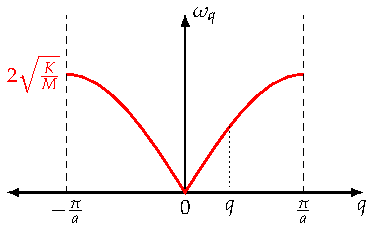
\includegraphics[]{Images/fig-monochaindispersion.pdf}
    \caption{Dispersion relation for the monoatomic chain.}
    \label{fig-monochaindispersion}
\end{figure}

\newpage 
\subsection{Example 2 - Diatomic Chain}

\begin{figure}[htbp]
    \centering
    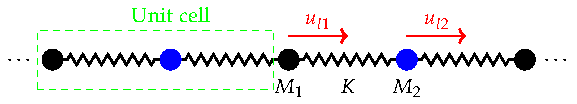
\includegraphics[]{Images/fig-diachaincartoon.pdf}
    
    \caption{A diatomic chain. We have alternating atoms of mass $M_1/M_2$ joined by springs of spring constant $K$. We index the displacement of the $M_1$ atoms with $u_{l_1}$ and the $M_2$ atoms as $u_{l_2}$. A unit cell contains one atom of each type and two springs.}
    \label{fig-diachaincartoon}
\end{figure}
We now consider a diatomic chain. We now have two different types of atoms in our chain; mass $M_1$ and mass $M_2$. The springs between them are still of spring constant $K$. The unit cell contains one atom of each type and two of the springs. We denote the displacement of the $M_1$ atoms as $u_{l_1}$ and the $M_2$ atoms as $u_{l_2}$.



Similar analysis as before gives the momentum space dynamical matrix (Check!):
\begin{equation}
    V_q = \m{2K & -K(1-e^{iqa}) \\ -K(1+e^{-iqa}) & 2K}
\end{equation}
The Hamiltonian that follows from this is:
\begin{equation}
    H = \sum_q \left(\frac{p_{q_1}^\dag p_{q_1}}{2M_1} + \frac{p_{q_2}^\dag p_{q_2}}{2M_2}\right) + \frac{1}{2}\sum_{q}\m{\mu_{q_1}^\dag & \mu_{q_2}^\dag} V_{q}\m{\mu_{q_1} \\ \mu_{q_2}}
\end{equation}
this is typical for a more complicated chain, where $N$ different atoms would give an $N \times N$ $V_q$ matrix in momentum space. Another complication is that $M_1 \neq M_2$, and so it is not immediate to read off $\omega_q$; we need to get rid of unequal masses in the kinetic energy term. This is done through the rescaling of momenta:
\begin{equation}
    p_{q_1} \to p_{q_1}\left(\frac{M_1}{M_2}\right)^{1/4} \quad p_{q_2} \to p_{q_2}\left(\frac{M_2}{M_1}\right)^{1/4}
\end{equation}
This implies a corresponding scaling of the displacements:
\begin{equation}
    \mu_{q_1} \to \mu_{q_1}\left(\frac{M_2}{M_1}\right)^{1/4} \quad \mu_{q_2} \to \mu_{q_2}\left(\frac{M_1}{M_2}\right)^{1/4}
\end{equation}
so the Hamiltonian becomes:
\begin{equation}
    H = \sum_q \frac{p_{1q}^\dag p_{1q} + p_{2q}^\dag p_{2q}}{2\sqrt{M_1M_2}} + \frac{1}{2}\sum_q \m{\mu_{q_1}^\dag & \mu_{q_2}^\dag} \m{2K\sqrt{\frac{M_1}{M_2}} & -K(1+e^{iqa}) \\ -K(1+e^{-iqa}) & 2K\sqrt{\frac{M_2}{M_1}}}\m{\mu_{q_1} \\ \mu_{q_2}}
\end{equation}
the normal modes are given by eigenvalues of $\tilde{V}_q$ (the matrix in the potential energy term above):
\begin{equation}
    0 = \det(\tilde{V}_q - \omega\sqrt{M_1M_2}) = M_1M_2\omega^4 - 2K(M_1+ M_2)\omega^2 + 2K^2(1-\cos qa)
\end{equation}
This is just a quadratic equation in $\omega^2$, so:
\begin{equation}
    \omega_{12}^2 = \frac{2K}{M_1M_2}\left((M_1 + M_2) \pm \sqrt{(M_1 + M_2)^2 - 2M_1M_2(1 - \cos qa)}\right)
\end{equation}
If we sketch the dispersion realtion, we have:

\begin{figure}[htbp]
    \centering
    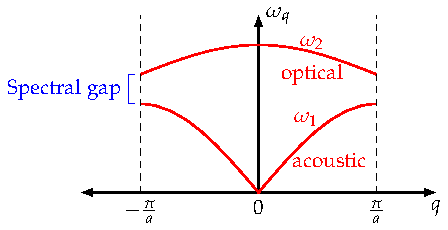
\includegraphics[]{Images/dig-diachaindispersion.pdf}

    \caption{Dispersion relations for diatomic chain. Note the presence of two different branches/phonon modes, and the spectral gap between them.}
    \label{fig-diachaindispersion}
\end{figure}

The acoustic branch is linear and the basis of sound waves inside of the material. The optical branch is excited by shining light on the material. If we shine waves of an intermediate energy in the spectral gap (in between hte two branches), none will propagate!

Next class, we will discuss phonons further; in particular how they behave in 3D, and thermodynamic properties of vibrating crystals.
\newpage
\section{Phonons in Three Dimensions}
% Logistics - MT on Nov. 2nd. Short in-class exam of 15-20 minutes of a few simple questions that everyone should know how to do. There is a practice MT. Takehome will be 3 problems, have until Nov. 7th to complete.
% Topics - We will finish phonons today, then discuss magnetic structure and magnons, then electrons in periodic potential and band structure theory. This will be the extent of the content covered.
\subsection{Review - The Real and Reciprocal 3D Lattice}
We consider atoms located at positions $\v{R}$ of a Bravais lattice in 3D space. Such a Bravais lattice can be written via:
\begin{equation}
    \v{R} = n_1\v{a}_1 + n_2\v{a}_2 + n_3\v{a}_3
\end{equation}
where $n_i \in \ZZ$ and $\v{a}_i$ are primitive vectors.

The corresponding reciprocal lattice vectors $\v{G}$ are defined by $e^{i\v{R} \cdot \v{G}} = 1$, which implies:
\begin{equation}
    \v{G} = m_1 \v{b}_1 + m_2\v{b}_2 + m_3\v{b}_3.
\end{equation}
Where $m_j \in \ZZ$ and $\v{b}_j$ are primitive vectors of the reciprocal lattice, satisfying the usual relation:
\begin{equation}
    \v{a}_i \cdot \v{b}_j = 2\pi \delta_{ij}.
\end{equation}

We will also need a relation:
\begin{equation}
    \sum_{\v{R}}e^{i\v{R} \cdot \v{q}} = N\sum_{\v{G}}\delta_{q\v{G}} = N\Delta (\v{q})
\end{equation}

\subsection{Writing down the 3D Hamiltonian}
The Hamiltonian for the 3d lattice with the harmonic approximation can be written as:
\begin{equation}
    H = \sum_{\v{R}, i}\frac{(p^i_\v{R})^2}{2M} + \frac{1}{2}\sum_{\v{R}, \v{R}'}\mu^i_\v{R} V_{\v{R}\v{R}'}^{ij}\mu^j_{\v{R}'}
\end{equation}
This is the expected generalization from 1D, where we see that the atoms can move and vibrate in three dimensions; $i, j \in \set{x,y,z}$. $V^{ij}_{\v{R}\v{R}'}$ (as before) is the dynamical matrix $V_{\v{R}\v{R'}}^{ij} = \left.\frac{\partial^2 V}{\partial \mu_\v{R}^i \partial \mu_{\v{R}'}^j} \right|_{\gv{\mu} = 0}$. We define the displacement/momenta at each lattice site as:
\begin{equation}
    \begin{split}
        \v{Y}_\v{R} &= \m{\mu_\v{R}^x \\ \mu_\v{R}^y \\ \mu_{\v{R}}^z}
        \\ \v{P}_\v{R} &= \m{p_\v{R}^x \\ p_\v{R}^y \\ p_{\v{R}}^z}
    \end{split}
\end{equation}
And therefore the Hamiltonian becomes:
\begin{equation}
    H = \frac{1}{2M}\sum_\v{R}\v{P}^T_\v{R} \v{P}_\v{R} + \frac{1}{2}\sum_{\v{R},\v{R}'}\v{Y}^T_\v{R} \m{V_{\v{R}\v{R}'}^{xx} & V_{\v{R}\v{R}'}^{xy} & V_{\v{R}\v{R}'}^{xz} \\ V_{\v{R}\v{R}'}^{yx} & V_{\v{R}\v{R}'}^{yy} & V_{\v{R}\v{R}'}^{yz} \\ V_{\v{R}\v{R}'}^{zx} & V_{\v{R}\v{R}'}^{zy} & V_{\v{R}\v{R}'}^{zz}} \v{Y}_{\v{R}}
\end{equation}
note that due to the definition of the dynamical matrix elements, the matrix appearing in the above expression is a real symmetric matrix.

\subsection{Translation Invariant Solution}
With the assumption of translation invariance, we obtain the condition $V^{ij}_{\v{R}\v{R}'} = V^{ij}_{\v{R} - \v{R}'}$. As we did for the 1D case, we will use a fourier transform:
\begin{equation}
    \v{Y}_\v{q} = \frac{1}{\sqrt{N}}\sum_{\v{R}}e^{-i\v{q} \cdot \v{R}}Y_\v{R}, \quad \v{P}_\v{q} = \frac{1}{\sqrt{N}}\sum_\v{R}e^{i\v{q} \cdot \v{R}}\v{P}_{\v{R}}
\end{equation}
As in 1D, we also have the periodicity:
\begin{equation}
    \v{Y}_{\v{q} + \v{G}} = \v{Y}_{\v{q}}, \quad \v{P}_{\v{q} + \v{G}} = \v{P}_\v{q}
\end{equation}
This defines the 3D Brillouin zone $\mathcal{B}$ as the fundamental domain of $\v{q}$. The Inverse FT gives:
\begin{equation}
    \v{Y}_\v{R} = \frac{1}{\sqrt{N}}\sum_{\v{q} \in \mathcal{B}}e^{i\v{q} \cdot \v{R}}\v{Y}_\v{q}, \quad \v{P}_\v{R} = \frac{1}{\sqrt{N}}\sum_{\v{q} \in \mathcal{B}}e^{-i\v{q} \cdot \v{R}}\v{P}_\v{q}
\end{equation}
The Hamiltonian reduces to:
\begin{equation}
    H = \sum_{\v{q} \in \mathcal{B}} \left(\frac{1}{2M}\v{P}^\dag_\v{q} \v{P}_\v{q} + \frac{1}{2}\v{Y}_q^\dag \m{V_{\v{q}}^{xx} & V_{\v{q}}^{xy} & V_{\v{q}}^{xz} \\ V_{\v{q}}^{yx} & V_{\v{q}}^{yy} & V_{\v{q}}^{yz} \\ V_{\v{q}}^{zx} & V_{\v{q}}^{zy} & V_{\v{q}}^{zz}}\v{Y}_\v{q}\right)
\end{equation}
where the $3N \times 3N$ matrix in the original basis has now reduced to a $3 \times 3$ matrix. The matrix elements in this basis are:
\begin{align*}
    \v{V}_{\v{q}}^{ij} = \sum_{\v{R}'}e^{i\v{q} \cdot (\v{R} - \v{R}')}V_{\v{R}\v{R}'}^{ij}
\end{align*}
To complete this solution, we have to diagonalize the $3 \times 3$ dynamical matrix. It is a Hermitian matrix and thus has three orthogonal vectors $\v{s}_1, \v{s}_2, \v{s}_3$ belonging to eigenvalues $\v{v}^1_\v{q}, \v{v}^2_\v{q}, \v{v}^3_\v{q}$. In this basis defined by these three orthogonal vectors, we have:
\begin{equation}
    H = \sum_{\v{q}, \mu=1,2,3}\left(\frac{p_q^{\mu\dag}p_q^\mu}{2M} + \frac{1}{2}V_q^\mu \mu_q^{\mu^\dag}\mu^\mu_q\right)
\end{equation}
where $\mu_q^\mu = \gv{\mu}_\v{q} \cdot \v{s}_\mu$ and $p_q^\mu = \v{p}_\v{q} \cdot \v{s}_\mu$. 

The 3 directions described by $\v{s}_\mu(\v{q})$ define phonon \emph{polarization}. In addition, for $\v{q}$ along a high-symmetry axis, we typically have $\v{s} \parallel \v{q}$ which is a ``longitudinal phonon'' and $\v{s} \perp \v{q}$ which is two ``transverse phonons''.

Why a high symmetry axis? If we take an arbitrary $\v{q}$ pointing in some random direction in reciprocal space, in general none of the $\v{s}$ will be parallel to $\v{q}$ or orthogonal to it. But when the phonon propogates along a high symmetry axis, we do typically see this separation.

Phonon frequencies are given by:
\begin{equation}
    \omega_{\v{q}\mu} = \sqrt{\frac{V_\v{q}^\mu}{M}}
\end{equation}
and the corresponding raising/lowering operators are:
\begin{equation}
    a_{\v{q}\mu} = \frac{1}{\sqrt{2M\hbar \omega_{\v{q}\mu}}}(M\omega_{\v{q}\mu}\mu^\mu_\v{q} + ip_\v{q}^{\mu\dag}), \quad a_{\v{q}\mu}^\dag = \ldots
\end{equation}
which leads to:
\begin{equation}
    H = \sum_{\v{q}, \mu}\hbar \omega_{\v{q}\mu}(a^{\dag}_{\v{q}\mu}a_{\v{q}\mu} + \frac{1}{2})
\end{equation}

One more comment before moving onto the next topic; this was all for a simple Bravais lattice. This is the simplest possible type of crystal structure where you have one type of atom periodically repeating in space. Most solids are not quite so simple and have a larger unit cell, such as Sodium Chloride. Things would work out exactly the same in this case, there would just be an additional index labelling the position of the atom inside the unit cell (of which there are $n_b$). The $3 \times 3$ matrix would become a larger $3n_b \times 3n_b$ matrix with $3n_b$ eigenvalues/eigenvectors, which describe the internal degrees of freedom in the unit cell. Previously, we had 3 polarizations for the one atom type. Now we have 3 polarizations per atom type, so there is a more complex structure with more modes (e.g. different atoms can vibrate in different directions). Of these, 3 will be acoustic modes (frequency goes to zero as $\v{q} \to \v{0}/\lambda \to \infty$), and $3(n_b - 1)$ will be acoustic modes.

\begin{figure}[htbp]
    \centering
    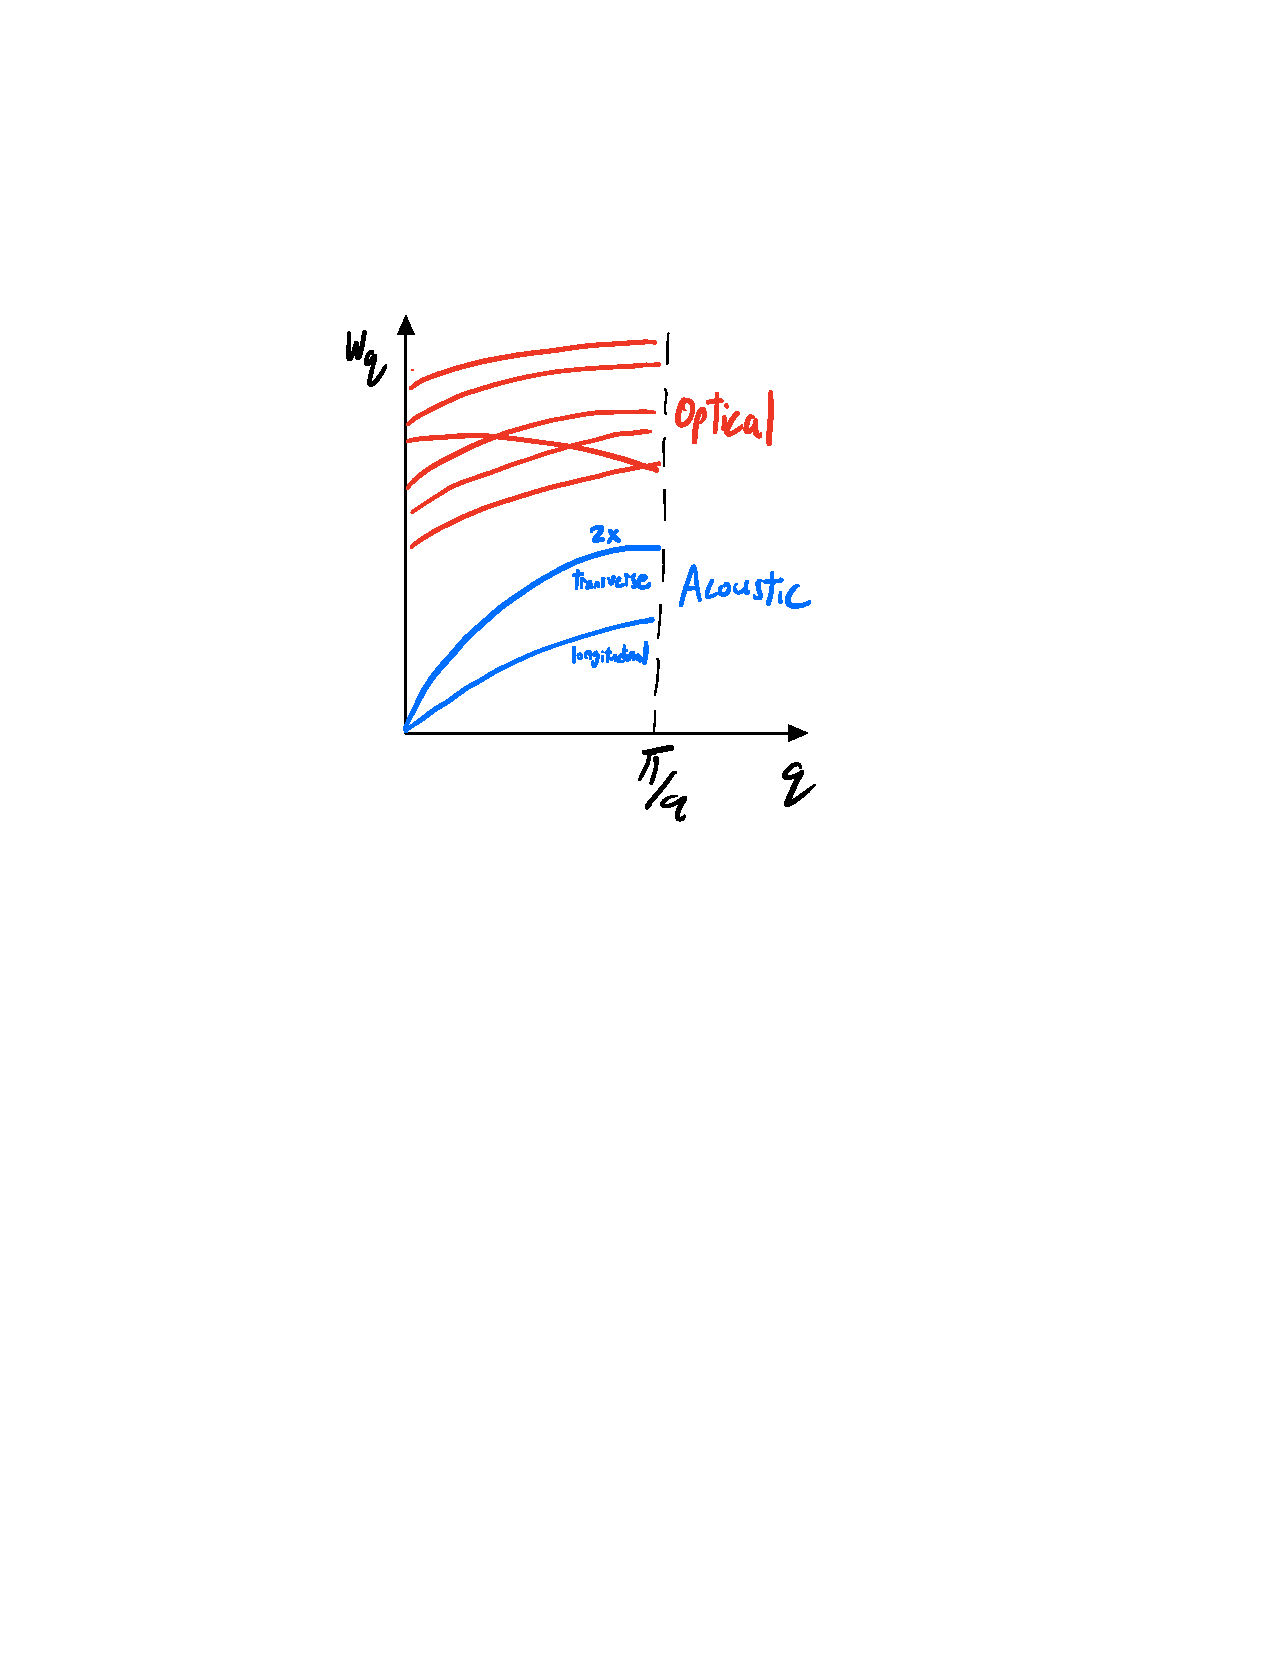
\includegraphics[scale=0.7]{Images/fig-3dphonondispersion.pdf}

    \caption{Plot of the phonon dispersion curves for a complex 3d solid. We have 3 acoustic modes (1 longitudinal mode and 2 degenerate transverse modes) and $3(n_d - 1)$ optical modes. }
    \label{fig-3dphonondispersion}
\end{figure}

\subsection{Debye Model, Specific Heat of Phonons}
This was one of the main puzzles in solid-state physics before the advent of QM! Let's figure out how to calculate this. The internal energy in lattice vibrations is given by:
\begin{equation}
    U = \avg{H}_\beta = \sum_{\v{q}\mu}\hbar \omega_{\v{q}\mu}(\avg{a^\dag_{\v{q}\mu}a_{\v{q}\mu}} + \frac{1}{2})
\end{equation}
Where $\avg{a^\dag_{\v{q}\mu}a_{\v{q}\mu}} = \bar{n}_{\v{q}\mu} = \frac{1}{e^{\beta \hbar \omega_{\v{q}\mu}} - 1}$ is the bose-einstein occupation factor. It will actually be easier to go straight to the heat capacity:
\begin{equation}\label{eq-photonCV}
    C_V = \dod{U}{T} = \frac{1}{k_B T^2}\sum_{\v{q}, \mu}\frac{(\hbar \omega_{\v{q}\mu})^2 e^{\beta \hbar \omega_{\v{q}\mu}}}{(e^{\beta\hbar\omega_{\v{q}\mu}} - 1)^2}
\end{equation}
to evaluate the sum we would need to know the form of $\omega_{\v{q}\mu}$, and even then there usually does not exist a closed-form solution for the summation.

To evaluate Eq. \eqref{eq-photonCV}, it is useful to define the phonon density of states:
\begin{equation}
    D(\omega) = \sum_{\v{q}, \mu} \delta(\omega - \omega_{\v{q}\mu})
\end{equation}
This implies:
\begin{equation}
    C_V = \frac{1}{k_BT^2}\int_0^\infty d\omega D(\omega)\frac{(\hbar\omega)^2 e^{\beta\hbar\omega}}{(e^{\beta\hbar\omega} - 1)^2}
\end{equation}
The Debye model assumes $\omega_{\v{q}\mu} = c_\mu\abs{\v{q}}$, approximating the acoustic modes as straight lines. It should be accurate at low $T$ when only low frequency acoustic phonons are thermally excited. For simplicity, we further assume equal velocities $c_\mu = c$ for $\mu = 1,2,3$ (but this is not essential, and the calculation can still be done). We then get:
\begin{equation}
    \begin{split}
        D(\omega) &= \frac{3V}{(2\pi)^3}\int d^3q \delta(\omega - cq)
        \\ &= \frac{3V}{(2\pi)^3}4\pi \int q^2 dq \delta(\omega - cq) 
        \\ &= \frac{3V}{3\pi^2}\frac{\omega^2}{c^3}.
    \end{split}
\end{equation}
where the $3$ comes from the 3 directions summed over and we evaluate the integral by going into spherical coordinates. 

\subsection{Debye Frequency, Momentum, Temperature}
There is one more constraint for us to accomodate. The density of states has the property that if we integrate over it, we should get the total number of modes in the entire system (which in this case should be $3N$; $N$ particles moving in three dimensions). Therefore, the above expression cannot go on forever; and this is evident from the acoustic spectra where we see there are no states above some energy. So, we introduce a Debye frequency $\omega_D$:
\begin{equation}
    D(\omega) = \begin{cases}
        \frac{3V}{2\pi^2}\frac{\omega^2}{c^3} & \Omega < \omega_D
        \\ 0 & \omega > \omega_D
    \end{cases}
\end{equation}
where $\omega_D$ is determined by:
\begin{equation}
    \int_0^{\omega_D}D(\omega)d\omega = 3N \implies \omega_D^3 = 4\pi^2c^3\frac{N}{V}
\end{equation}'

\begin{figure}[htbp]
    \centering
    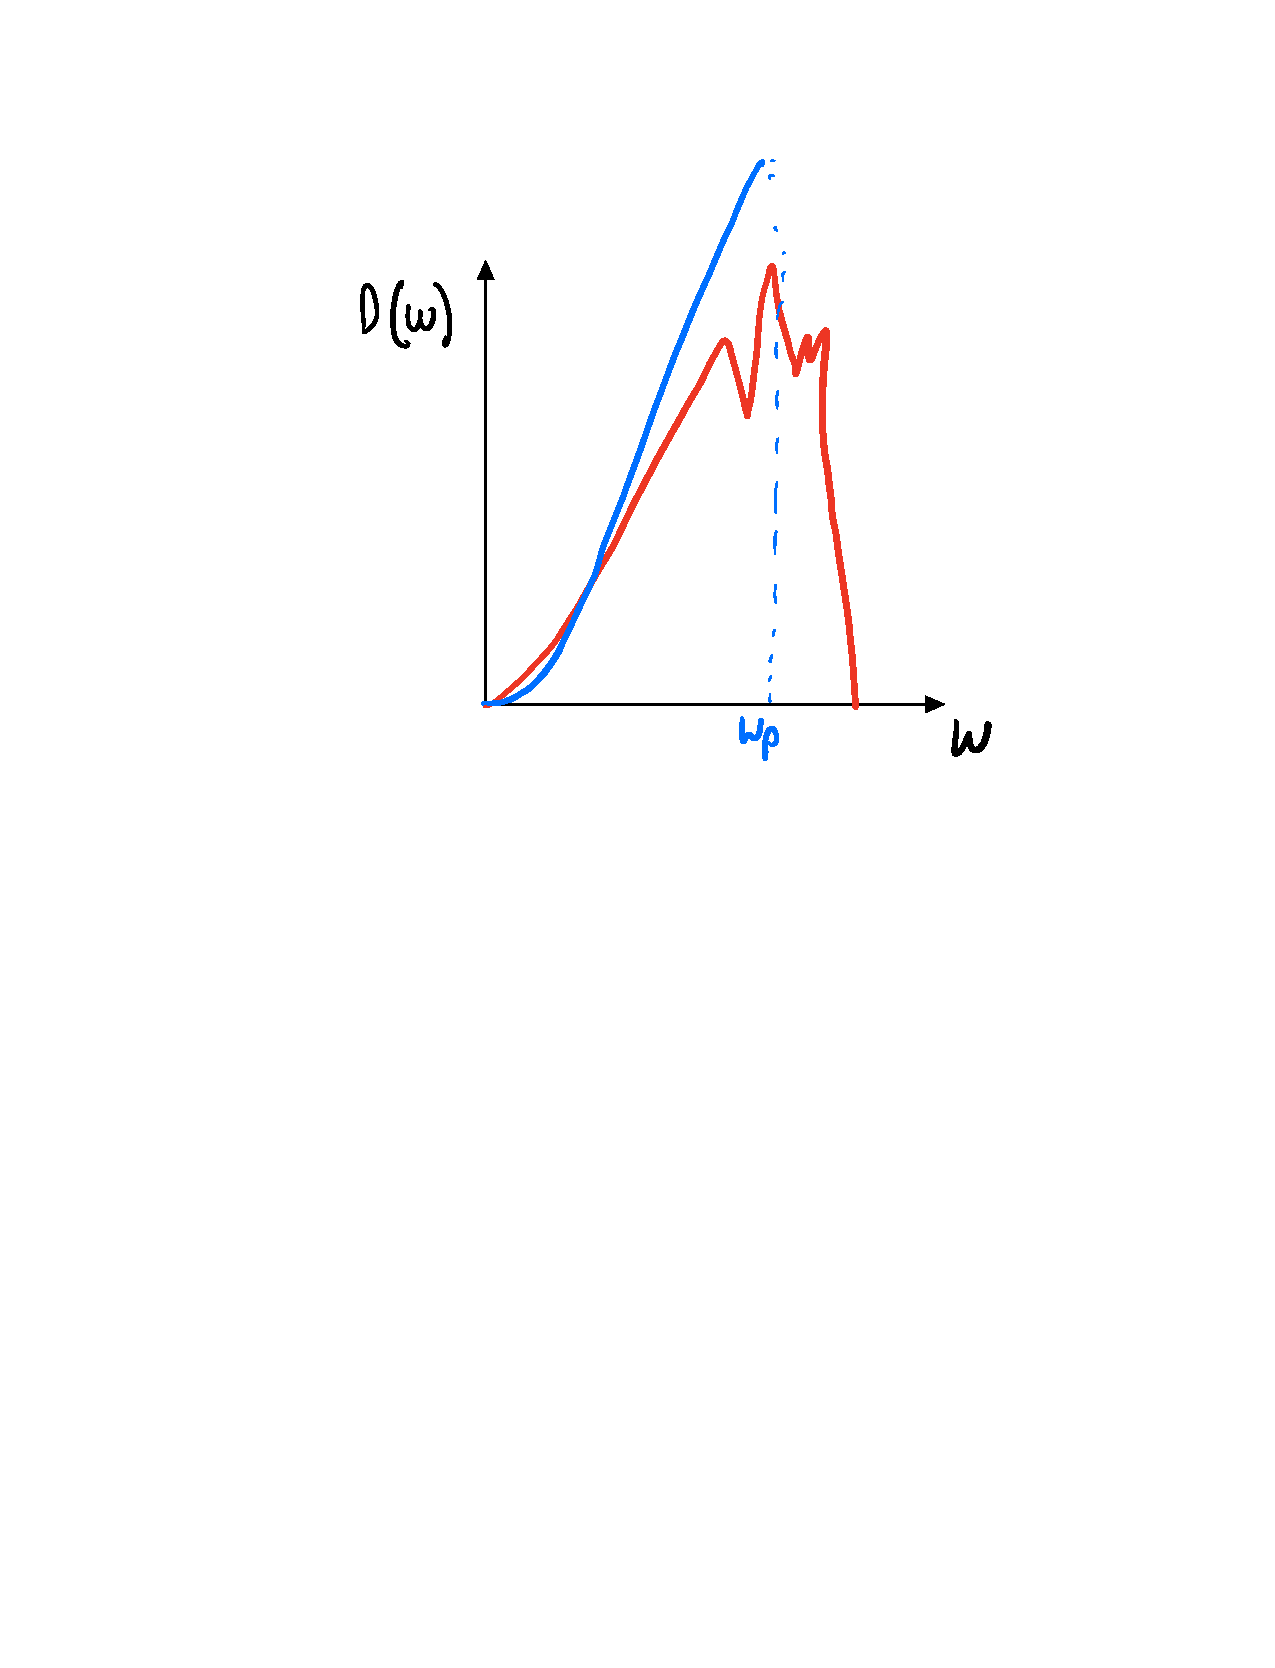
\includegraphics[scale=0.6]{Images/fig-phonondensityofstates.pdf}

    \caption{Plot of a realistic/experimentally measured phonon density of states (red) and our approximate calculated value (blue). We cut off the $\omega^2$ prediction for the density of the states at the Debye frequency $\omega_D$ such that the area under the curve (i.e. the total number of modes) is $3N$ (and the same for the two plots). It may seem like we neglect a lot of structure in making our approximation, but since we are itnerested in the heat capacity $C_V$, this complex structure generally gets smeared out regardless; hence our approximation can give reasonable predictions for heat capacity.}
    \label{fig-phonondensityofstates}
\end{figure}

This notion of a Debye frequency turns out to be very useful. It also defines Debye momentum:
\begin{equation}
    k_D = \frac{\omega_D}{c} = \left(6\pi^2\frac{N}{V}\right) \sim \frac{4}{a}
\end{equation}
where $a$ is the lattice spacing. It also defines the Debye temperature:
\begin{equation}
    \Theta_D = \frac{\hbar\omega_D}{k_B} \sim 74\si{K} - 1800\si{K}
\end{equation}
where $74\si{K}$ corresponds to Pr and $1800\si{K}$ corresponds to diamond. On average it is on the order of a few hundred Kelvin. These are all characteristic scales of phonons. Of all of them, Debye temperature tends to be the most useful as it is in the most tangible units. It distinguishes a low and high temperature regime for phonon excitations (i.e. the frequency for which below it the acoustic approximation is reasonable)

\subsection{Back to Heat Capacity}
We have:
\begin{equation}
    \begin{split}
        C_V &= \frac{3V\hbar^2}{2\pi^2c^2k_BT^2}\int_0^{\omega_B}d\omega \frac{\omega^4 e^{\beta\hbar\omega}}{(e^{\beta\bar\omega} - 1)^2}
        \\ &= gNk_B\left(\frac{T}{\theta_D}\right)^3\int_0^{\theta_D/T} dx \frac{x^4e^x}{(e^x - 1)^2}
    \end{split}
\end{equation}
where we have made the substitution $x = \beta\hbar\omega$. We call the integral $f(\theta_D/T) = f(x_D)$ the Debye function.

We now analyze some consequences. In principle we can solve the integral numerically, but we can also start by studying the integral analytically in two limits.

\subsubsection{Low T behavior}
In this limit we have $T \ll \theta_D$ and hence $x_D = \frac{\theta_D}{T} \gg 1$. We can therefore write:
\begin{align*}
    f(x_D) = \int_0^\infty \frac{x^4 e^x}{(e^x - 1)^2} - \int_{x_D}^\infty \frac{x^4 e^x}{(e^x - 1)^2} \approx \frac{4\pi^4}{15} - \int_{x_D}^\infty x^4 e^{-x} \approx \frac{4\pi^4}{15}
\end{align*}
where we have evaluated the first term analytically (calculus exercise) and the second integral we have that $x \gg 1$ over the rande of integration and we may therefore approximate $\frac{x^4e^x}{(e^x - 1)^2} \approx x^4 e^{-x}$. Since this is an exponentially small term, we can drop it. The specific heat then becomes:
\begin{equation}
    C_V \approx \frac{12\pi^4}{5}Nk_B\left(\frac{T}{\theta_D}\right)^3
\end{equation}
so for $T \ll \theta_D$ we find $C_V \sim T^3$. This is obeyed in many solids.

\subsubsection{High T behavior}
In this limit, we have $T \gg \theta_D$ and so $x_D \ll 1$. We therefore may expand $e^x$ to leading order in the integrand. This yields:
\begin{align*}
    f(x_D) \approx \int_0^{x_D}dx \frac{x^4}{(1+x-1)^2} = \int_0^{x_D} dx x^2 = \frac{1}{3}x_D^3
\end{align*}
where in the numerator we have approximated $e^x \sim 1$ and in the numerator we have approximated $e^x \sim 1 + x$.

So plugging this back into our specific heat expression:
\begin{equation}
    C_V \approx 3Nk_B
\end{equation}
so for $T \gg \theta_D$ we find that $C_V$ is independent of temperature. This is the Dulong-Petit law; this is the heat capacity of a harmonic crystal in classical theory (i.e. no quantum effects). If we recall the equipartition theorem, we have $N$ atoms oscillating in $3$ directions, so $3$ vibrational degrees of freedom and $3$ kinetic degrees of freedom and so $6N$ degrees of freedom in total. Equipartition associates $\frac{1}{2}k_B T$ per energy per degree of freedom and so we have $U = 6N \cdot \frac{1}{2}k_B T = 3Nk_B T$ of energy and hence $C_V = 3Nk_B$ specific heat. This of course in some sense makes sense as at high temperatures we expect quantum effects to be washed out and the system behaves basically classically (though an interesting point to note here - the quantum effect of the suppression of specific heat persists up to room temperature, as $\theta_D$ is on the order of hundreds of Kelvin; we do not have to cool our system to very low temperature for the quantum effects to become significant). This was known before QM was invented, but disagreed with experiment, where the specific heat went to zero at zero temperature (though it described the high-$T$ behavior well). With quantum mechanics, we are able to obtain a prediction that described experimental results very well.

\begin{figure}[htbp]
    \centering
    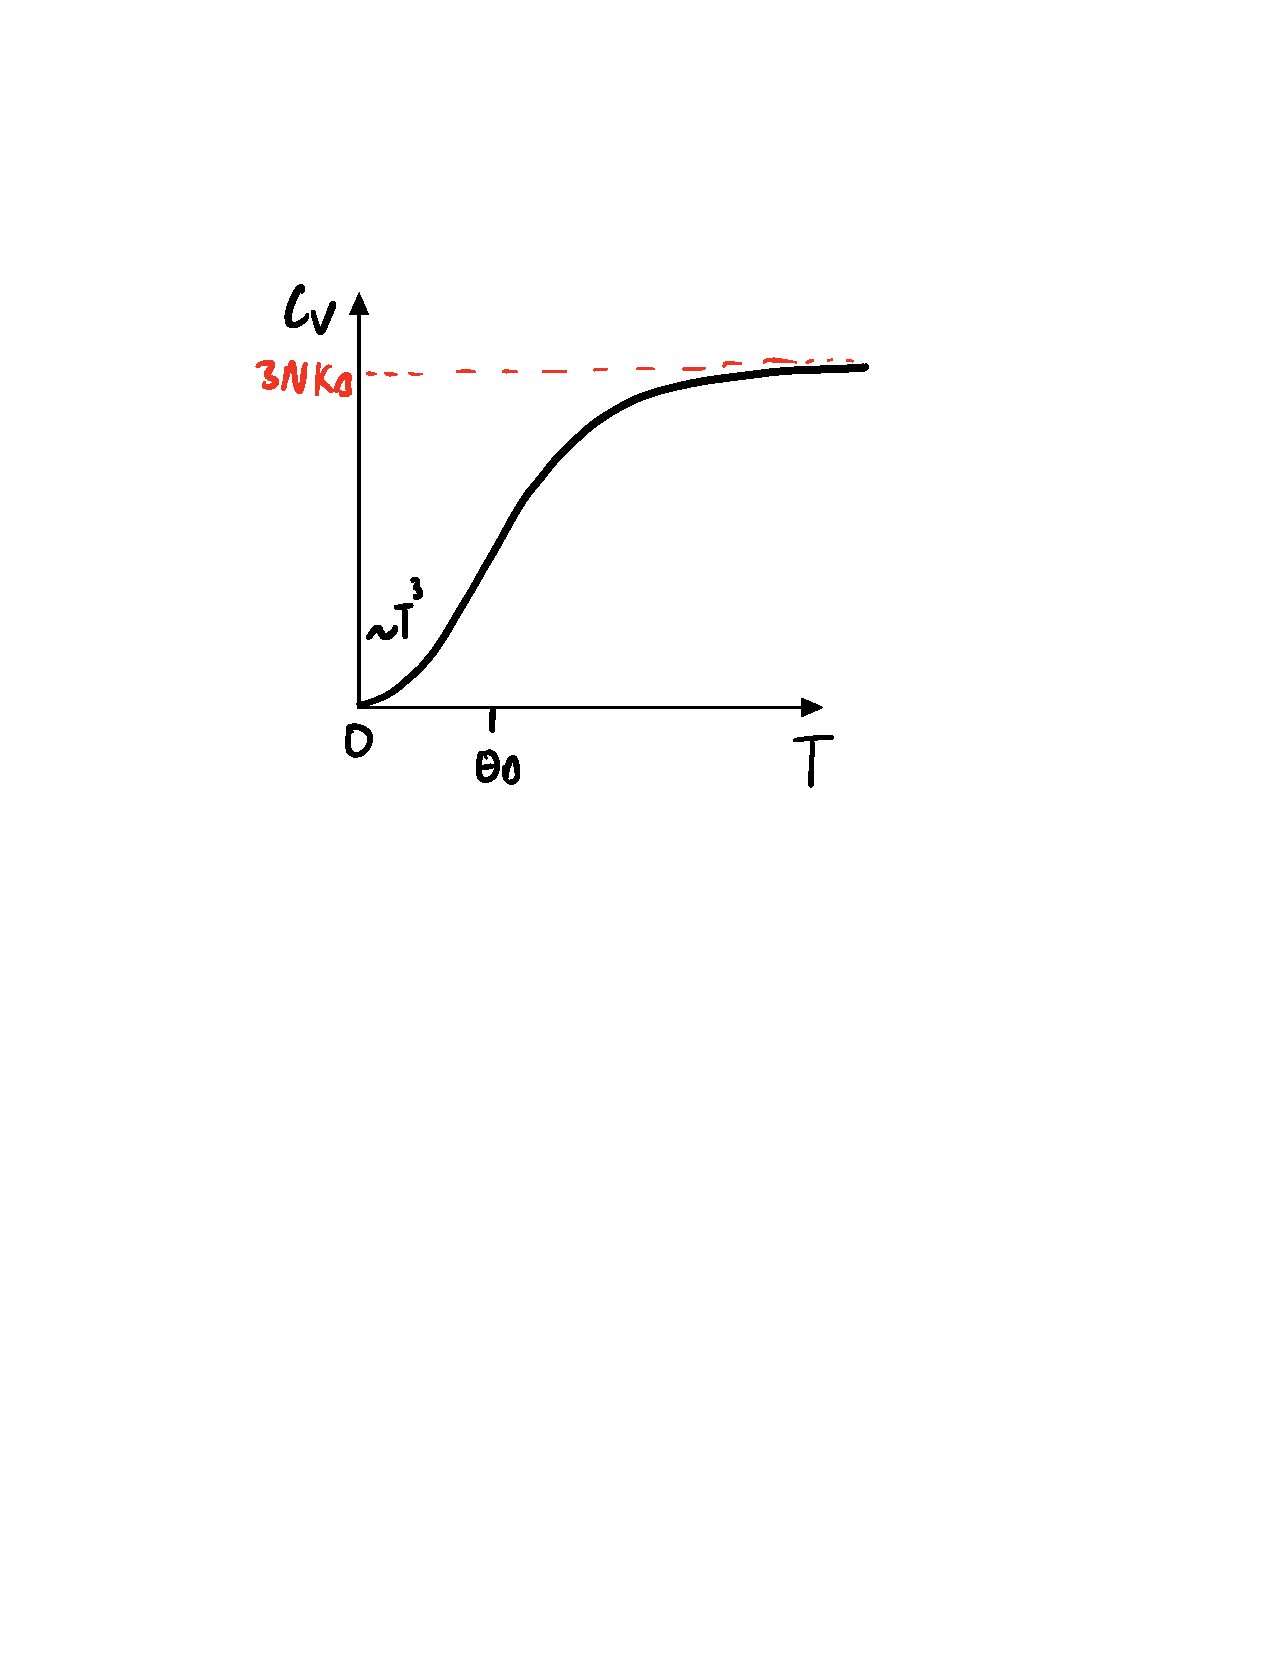
\includegraphics[scale=0.7]{Images/fig-phononspecificheat.pdf}

    \caption{Specific heat for phonons as a function of temperature $T$. At low $T$ we see $C_V \sim T^3$ behavior. At high $T$ we see that $C_V$ tends to a constant of $3Nk_B$.}
    \label{fig-phononspecificheat}
\end{figure}

\subsection{Einstein Model}
Is a model suitable for the study of optical phonons. We replace the dispersion relation for an optical phonon with an average $\omega_0$.

\begin{figure}[htbp]
    \centering
    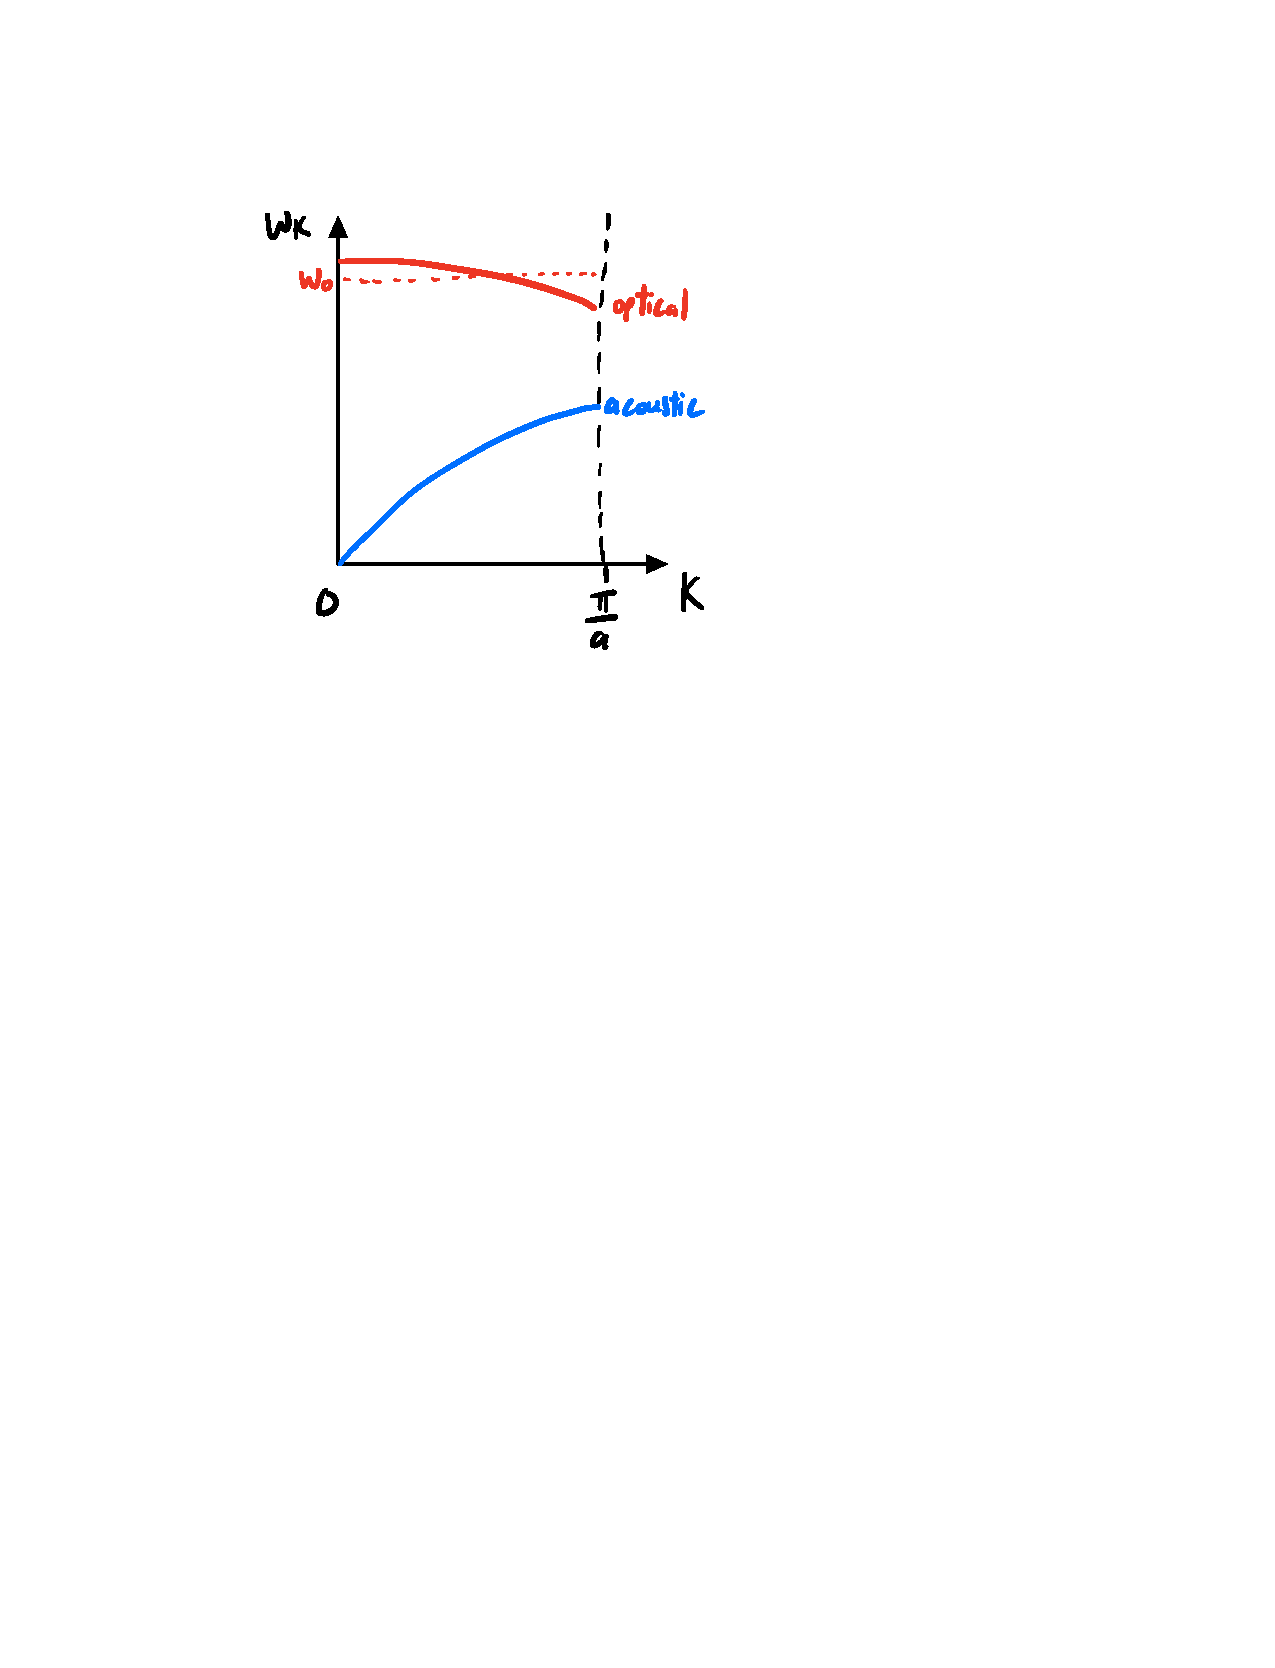
\includegraphics[scale=0.7]{Images/fig-einsteinmodelapprox.pdf}

    \caption{Dispersion relation for acoustic and optical modes of phonons, and Einstein's approximation for replacing the optical mode dispersion relation with a straight line at the average $\omega_0$.}
    \label{fig-einsteinmodelapprox}
\end{figure}


We consider an approximate phonon density of states:
\begin{align*}
    D(\omega) = N\delta(\omega - \omega_0)
\end{align*}
and from this we can calculate contribute to the heat capacity:
\begin{equation}
    C_V = \frac{1}{k_B T^2}\int_0^\infty d\omega\frac{(\hbar\omega)^2 e^{\beta\hbar\omega}}{(e^{\beta\hbar\omega} - 1)^2}D(\omega) = \frac{N}{k_BT^2}\frac{(\hbar\omega_0)^2 e^{\beta\hbar\omega_0}}{(e^{\beta\hbar\omega_0} - 1)^2}
\end{equation}
At low $T$, we have $\beta\hbar\omega_0 \gg 1$ and so:
\begin{equation}
    C_V \approx N k_B\left(\frac{\hbar\omega_0}{k_B T}\right)^2 e^{-\frac{\hbar\omega_0}{k_B T}}
\end{equation}
so we have ``exponentially activated behavior'' here.

\begin{figure}[htbp]
    \centering
    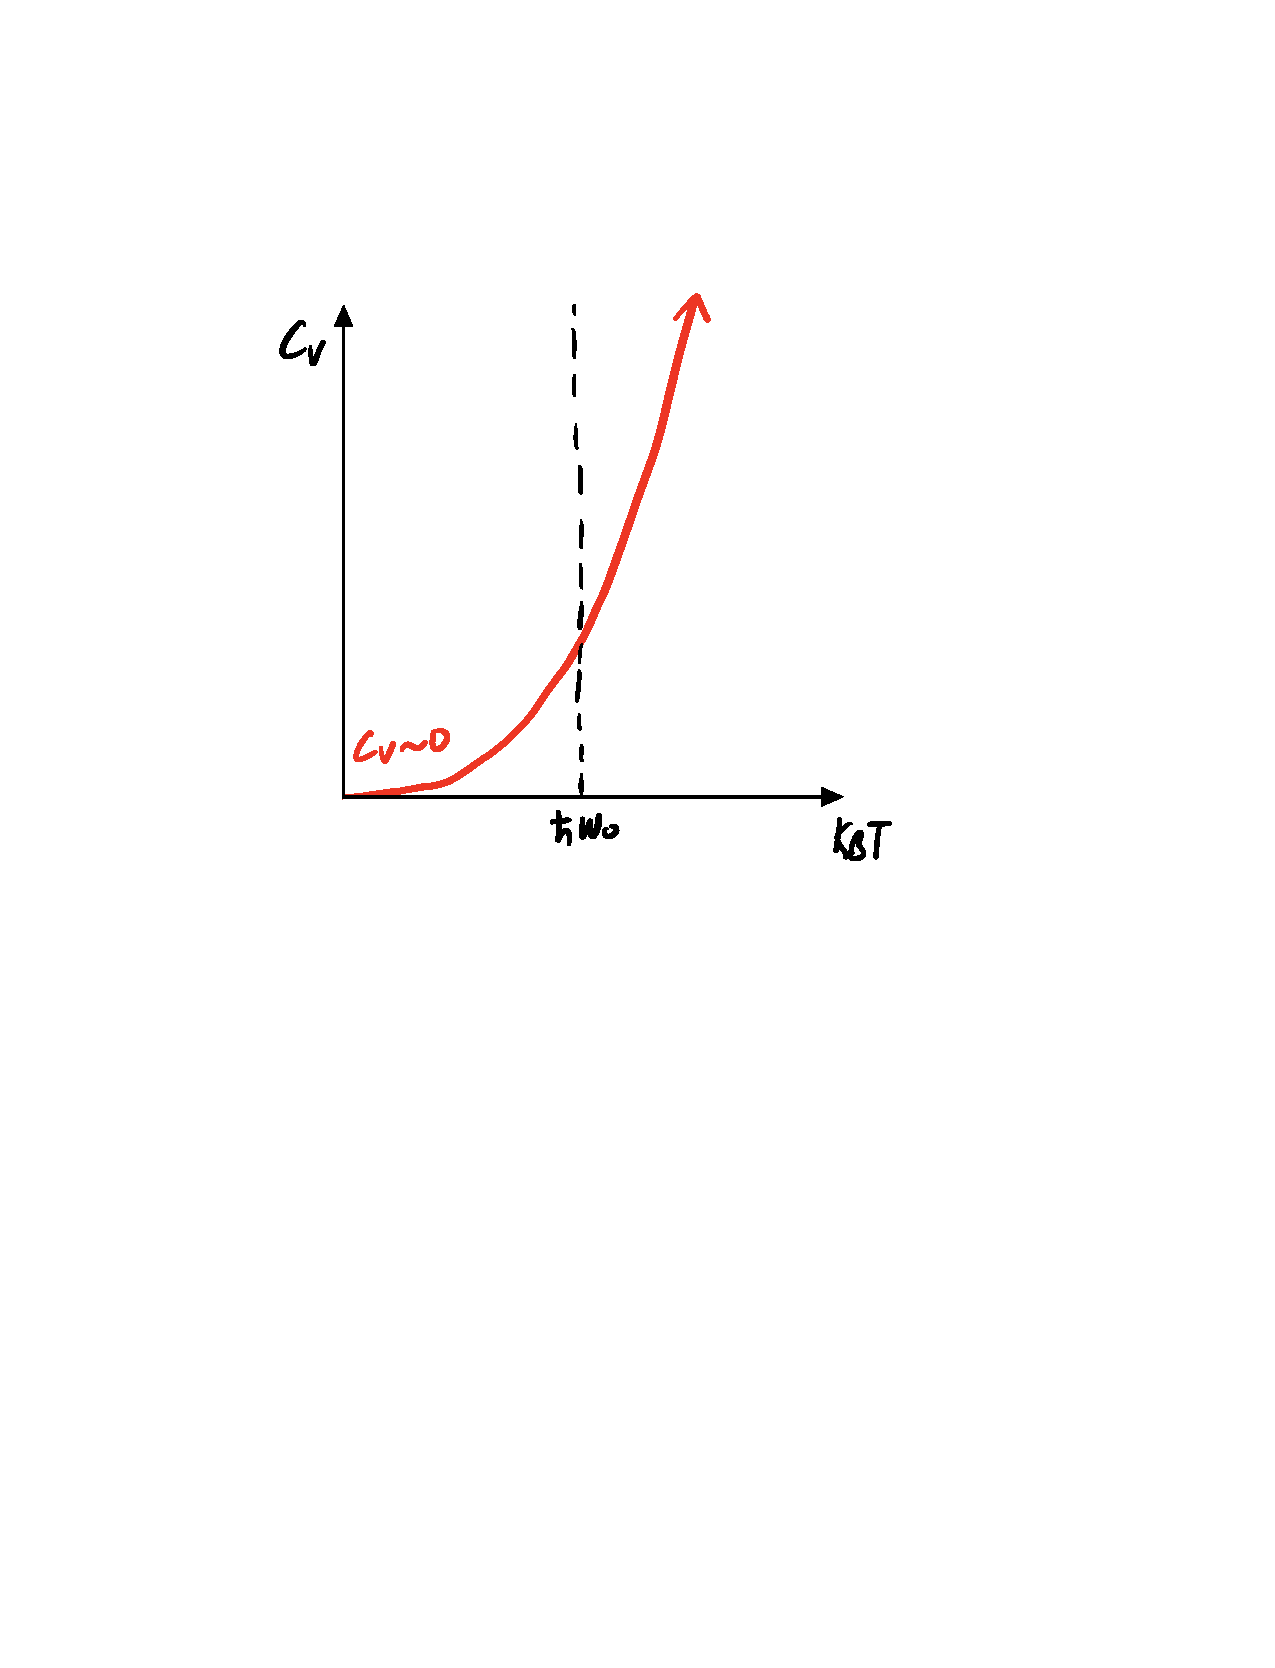
\includegraphics[scale=0.7]{Images/fig-einsteinmodelspecificheat.pdf}
    \caption{Plot of the low-$T$ specific heat as calculated by the Einstein model. We see the exponentially activated behavior, where past $\hbar\omega_0$ the specific heat sharply spikes.}
    \label{fig-einsteinmodelspecificheat}
\end{figure}

Interestingly, if we compare the two plots for the specific heat, they agree pretty well. Some differences at the very low $T$ limits, however. For the low $T$ einstein model at very low temperatures we do not even have one quantum of energy to excite, and so we have $C_V = 0$. Conversely, for the acoustic modes we are able to excite things at even very low temperatures (so long as the temperature is not zero).

\subsection{Anharmonic Effects and Phonon Interactions}
We take a step back and regard a solid (metal) as a collection of electrons (fermions) and phonons (bosons).

At low $T$, both the electrons and phonons contribute to thermodynamic (and other) properties, e.g. specific heat:
\begin{align*}
    C_V^{ph} \approx 6T^3 \text{ (Debye)}
\end{align*}
\begin{align*}
    C_V^{el} \approx aT \text{ (Sommerfield)}
\end{align*}
both are crucially quantum mechanical; if we forget quantum mechanics then these become temperature dependent constants. The total specific heat is the sum of the two:
\begin{align*}
    C_V = C^{el}_V + C^{ph}_V \approx aT + bT^3
\end{align*}
or:
\begin{equation}
    \frac{C_V}{T} \approx a + bT^2
\end{equation}
and many (most) metals behave in this way. This is a huge success of quantum theory and modern solid-state physics.

However, there are some significant failures of this model:
\begin{enumerate}
    \item Thermal expansion (Within the harmonic expansion, you can prove this does not occur)
    \item Thermal conductivity (Phonons to not carry heat in this model)
    \item Sound attenuation (Sound attenuates forever)
\end{enumerate}
but whenever our theories fail, we can look back to what approximations we have made, and see what things to improve. These three failures can be understood by incorporating anharmonic effects. In the harmonic approximation, we threw away all terms past the second derivative, but we could consider successive terms of order:
\begin{equation}
    H_3 = \frac{1}{3!}\sum_{RR'R''ijk}\mu_R^i \mu_{R'}^j \mu_{R''}^{k} V^{ijk}_{RR'R''}
\end{equation}
where:
\begin{equation}
    V^{ijk}_{RR'R''} = \left. \frac{\partial^3 V}{\partial \mu_R^i \partial \mu_{R'}^j \partial \mu_{R''}^k}\right|_{\mu=0}
\end{equation}

Note that the inclusion of these third-order terms is sufficient to describe thermal expansion and sound attenuation. To obtain thermal conductivity from the model, one needs to go to fourth order.

In translation-invariant systems, this can be expressed as:
\begin{equation}
    H_3 = \frac{1}{6\sqrt{N}}\left(\frac{\hbar}{2M}\right)^{3/2}\sum_{qq'q''ijk\mu\nu\lambda}\frac{S_\mu^i S_\nu^j S_\lambda^k}{(\omega_{q\mu}\omega_{q'\nu}\omega_{q''\lambda})^{1/2}}V^{ijk}_{qq'q''}\Delta (\v{q} + \v{q}' + \v{q}'') (a_{-q\mu}^\dag + a_{q\mu})(a^\dag_{-q'\nu} + a_{q'\nu})(a^\dag_{-q''\lambda} + a_{q''\lambda})
\end{equation}
This looks absolutely terrible, but people have come up with clever ways to analyze such Hamiltonians, namely through the graphical means of Feynman diagrams. Each of the product of three terms contains an annhilation and creation operator. If we were to multiply them out, we would get six terms, which could be represented as follows:


\begin{figure}[htbp]
    \centering
    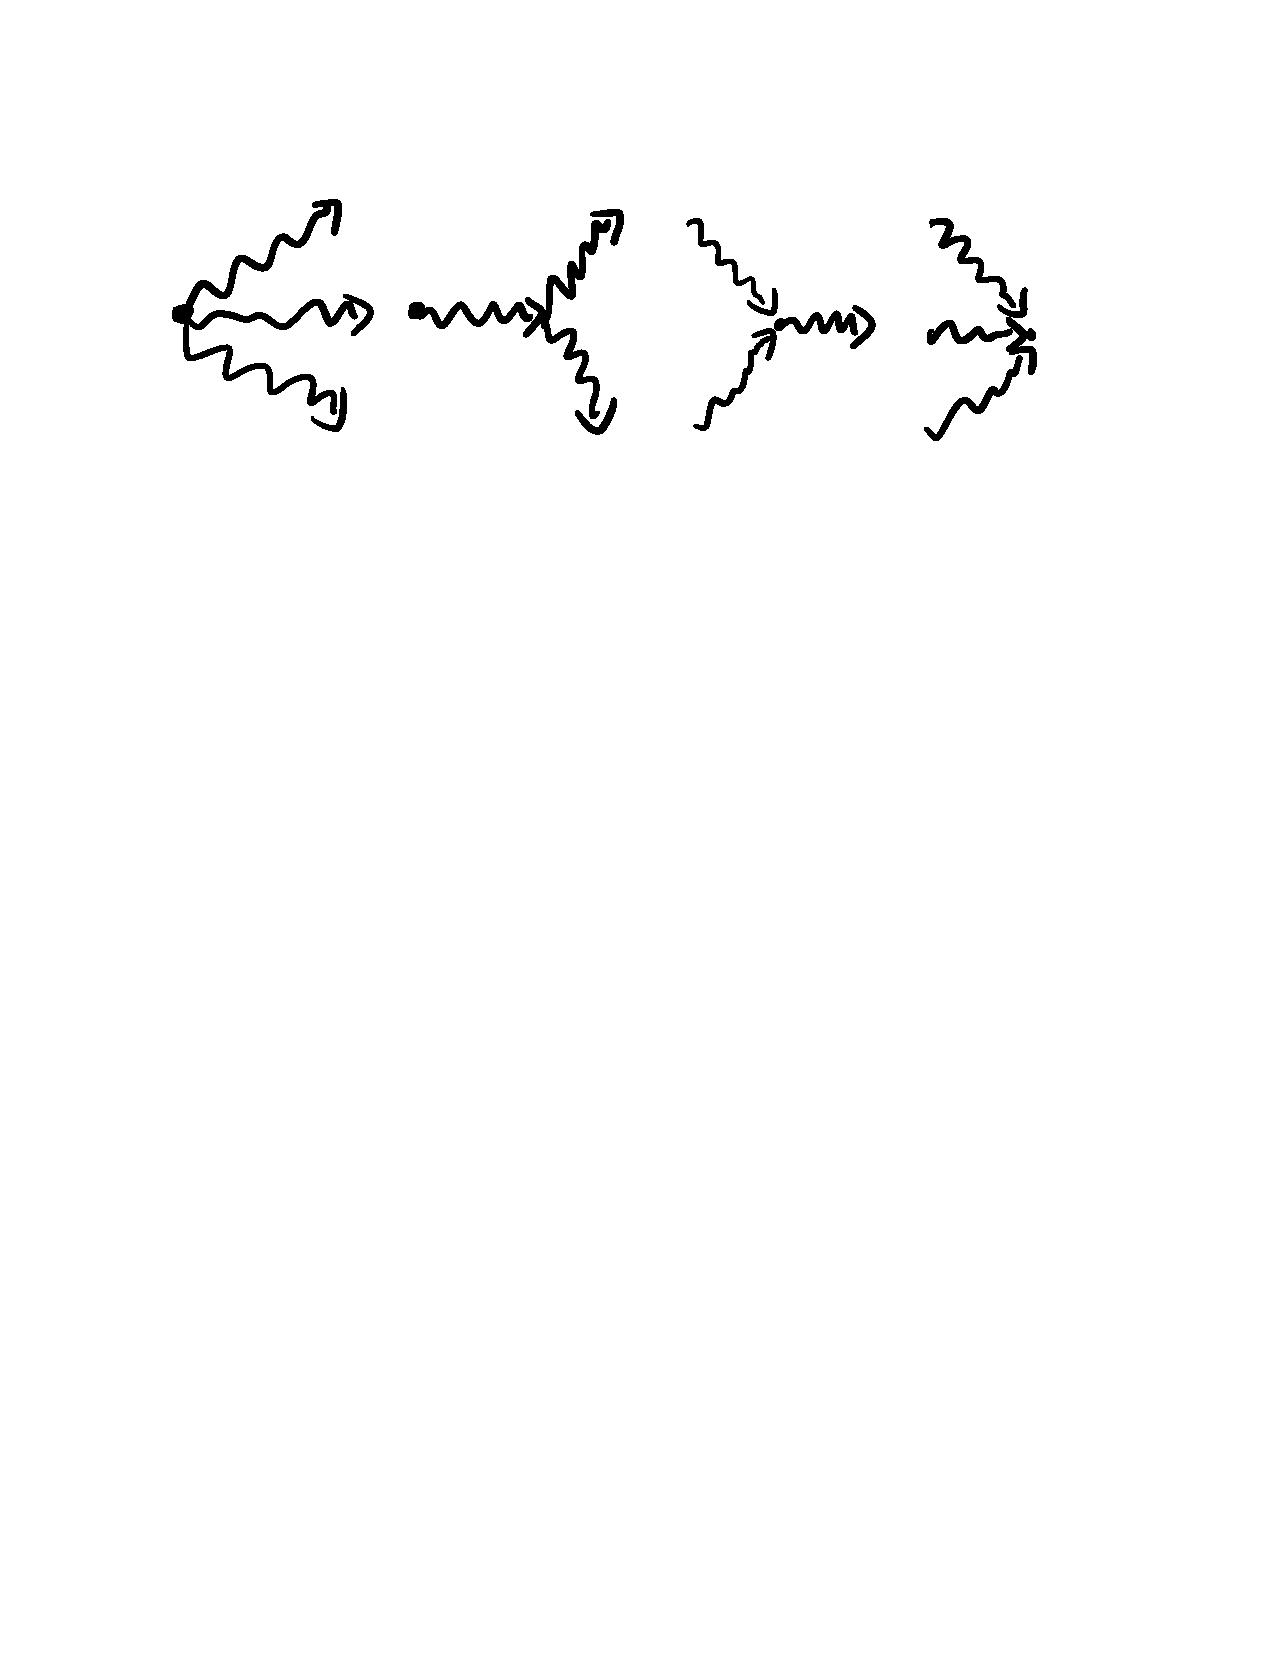
\includegraphics[scale=0.7]{Images/fig-threephonondiagrams.pdf}
    
    \caption{The four Feynman diagrams for three phonon interactions that come up in the third order term. In each diagram time runs from left to right. The leftmost diagram represents the creation of three phonons. The second diagram represents the destruction of one phonon and creation of two phonons. The third diagram represents the destruction of two phonons and creation of one phonon. Finally, the fourth diagram represents the destruction of three phonons.}
    \label{fig-threephonondiagrams}
\end{figure}

we can then assign a mathematical quantity to each of these diagrams, and thus evaluate each of their contributions in a clever way.

Without writing down the Hamiltonian, we can also look at the diagrams that arise in the fourth-order Hamiltonian $H_4$. We would have a product of four terms, which creates a sum with four phonons. Again, each of these diagrams could be assigned a mathematical quantity to evaluate their contribution.

\begin{figure}[htbp]
    \centering
    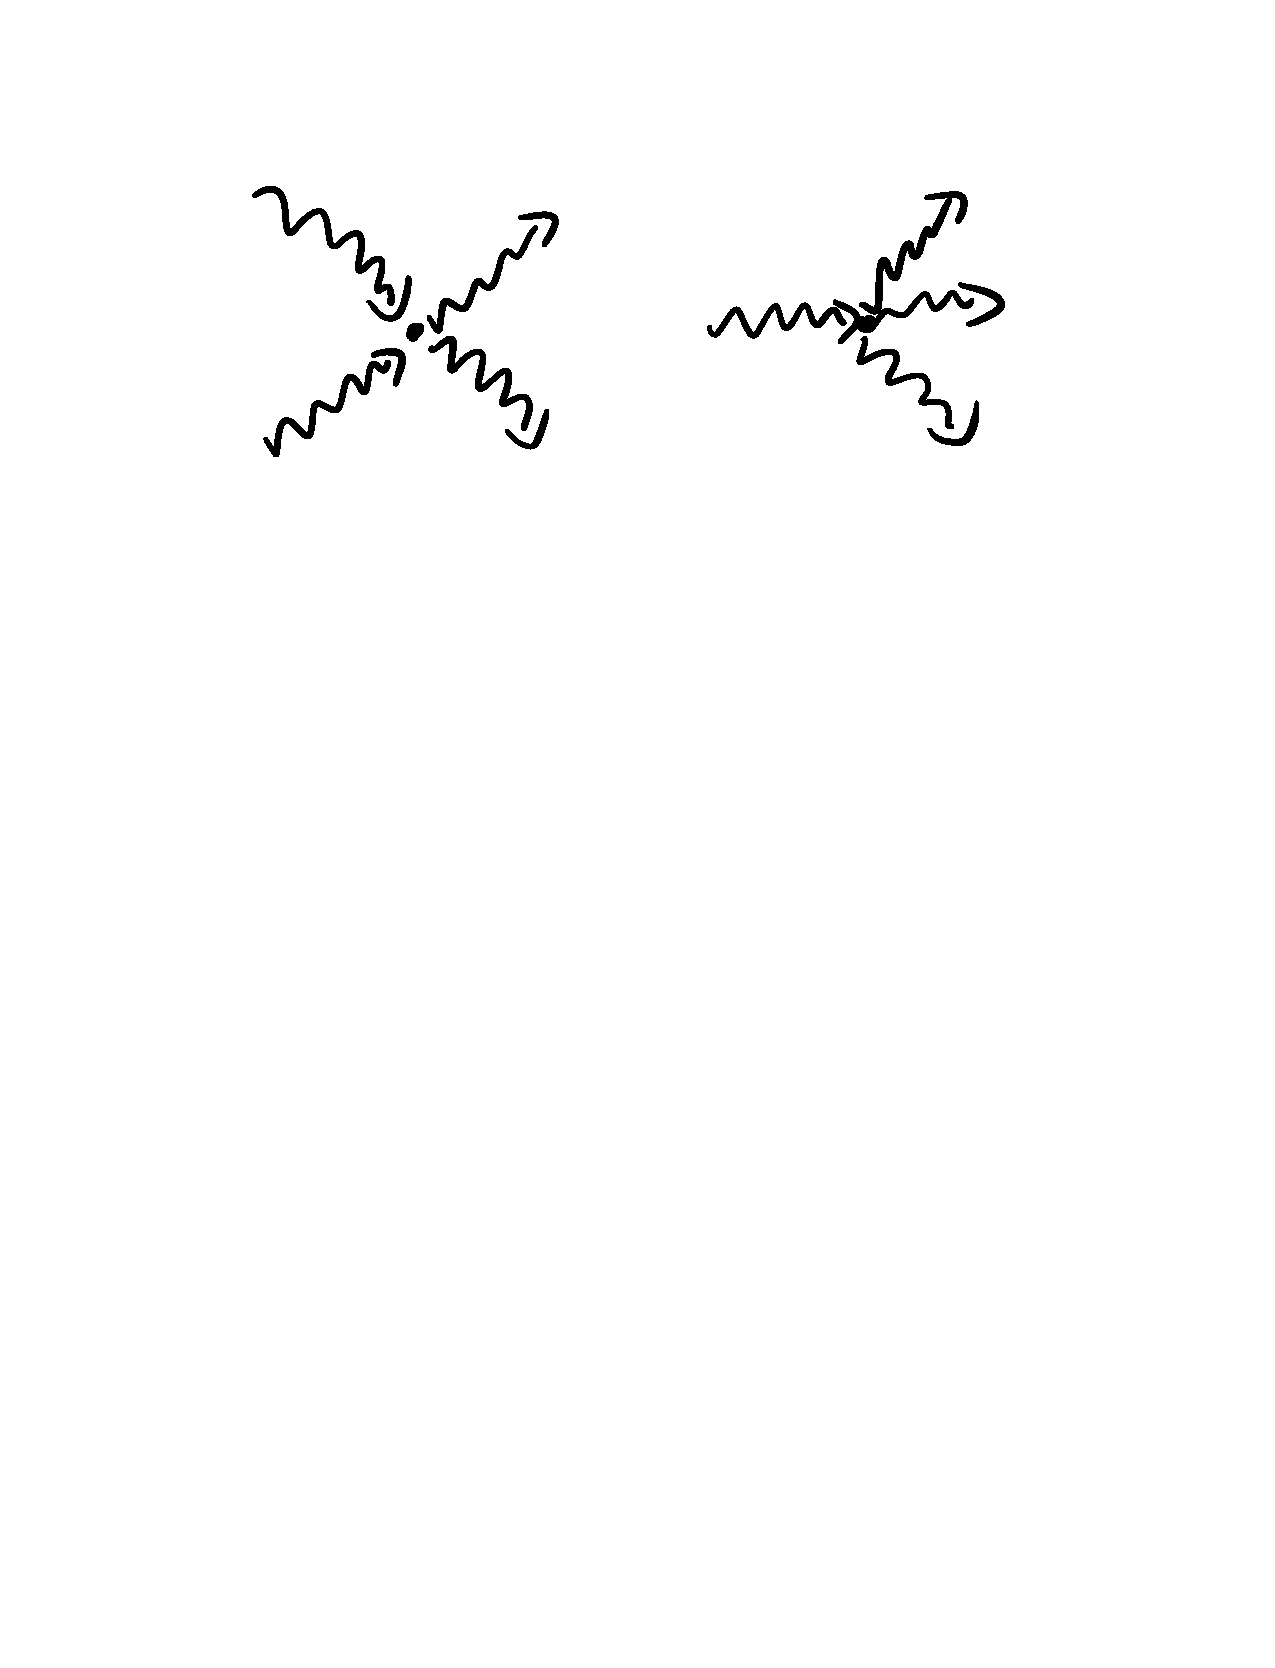
\includegraphics[scale=0.7]{Images/fig-fourphonondiagrams.pdf}
    
    \caption{Feynman diagrams for four phonon interactions that come up in the fourth order term. In each diagram time runs from left to right. The leftmost diagram represents the most dominantly contributing interaction, which is the scattering of two phonons. There are other interactions that also contribute, for example the destruction of one phonon and creation of three phonons as depicted in the right diagram.}
    \label{fig-fourphonondiagrams}
\end{figure}

\subsection{Thermal Conductivity}
In Drude theory, electrons contribute:
\begin{equation}
    \kappa_{el} = \frac{1}{3}C^{el}_V v_F l
\end{equation}
with $C^{el}_V$ the electronic specific heat, $v_F$ the Fermi velocity, and $l$ is the mean-free path - this is where many different details and factors come in (and generically very hard to calculate); this is where anharmonic effects enter. An electron that travelled forever would contribute an infinite conductivity - this does not happen so there must be features in our metal that slow it down, e.g. impurities. For phonons, we have (analogously)
\begin{equation}
    \kappa_{ph} = \frac{1}{3}C^{ph}_V c l'
\end{equation}
and again $l'$ the mean free path is where anharmonic effects enter (e.g. collisions of phonons with electrons).
\newpage
\setcounter{section}{10}
\section{Electrons in a Periodic Potential: Band Theory of Solids}

\subsection{Review: Bloch's Theorem}
See A\&M Ch. 8 for proof(s) and extended discussion.

\textbf{Theorem (Bloch).} Consider the eigenstates $\psi$ of the one-electron Hamiltonian:
\begin{align*}
    H = \frac{\hbar^2\nabla^2}{2m} + U(\v{r})
\end{align*}
where $U(\v{r} + \v{R}) = U(\v{r})$ for all $\v{R}$ in the Bravais lattice. These eigenstates can be chosen to have the form:
\begin{equation}\label{eq-Blocheigenstates}
    \boxed{\psi_{nk}(\v{r}) = e^{i\v{k}\cdot \v{r}}\mu_{nk}(\v{r})}
\end{equation}
where:
\begin{equation}\label{eq-Blocheigenstatesperiodic}
    \mu_{nk}(\v{r} + \v{R}) = \mu_{nu}(\v{r})
\end{equation} 

The interesting part of this statement is that even though the Haniltonian has a full symmetry under translation by $+ \v{R}$. The eigenstates do not; there is a part that possesses the symmetry $\mu_{nk}(\v{r})$ and a part that does not, $e^{i\v{k} \cdot \v{r}}$ which is translation invariant. This should not be totally unexpected; for example the QHO is symmetric under inversion, but the wavefunctions do not have all of this symmetry ($n$ even is even, $n$ odd is odd).

A remark: Note that Eqs. \eqref{eq-Blocheigenstates} and \eqref{eq-Blocheigenstatesperiodic} imply that:
\begin{equation}
    \psi_{nk}(\v{r} + \v{R}) = e^{i\v{k} \cdot \v{R}}\psi_{nk}(\v{r}).
\end{equation}

In Eq. \eqref{eq-Blocheigenstates}, $\v{k}$ is known as a crystal momentum and $n$ is the band index. In free space, complete translation invariance implies the conservation of momentum. In a lattice, we have translation invariance w.r.t the Bravais lattice $\v{R}$, only, which implies that momentum is not conserved, but the crystal momentum is conserved.

\subsection{Weak Periodic Potential}
This is also known as ``nearly free'' electrons in a periodic lattice. We consider the same Hamiltonian $H = \frac{\hbar^2\nabla^2}{2m} + U(\v{r})$ where $U(\v{r})$ is ``weak'', sufficiently weak enough to be treated in perturbation theory. We call $H_0 = \frac{\hbar^2\nabla^2}{2m}$ and $H' = U(\v{r})$.

First, we transform $H$ into second-quantized notation:
\begin{equation}
    \begin{split}
        H_0 &= \sum_{\v{k}, \sigma} \e_\v{k}c^\dag_{\v{k}\sigma}c_{\v{k}\sigma}, \quad \e_\v{k} = \frac{\hbar^2\v{k}^2}{2m}
        \\ H' &= \sum_{\v{k}\v{k}'\sigma\sigma'}\bra{\v{k}\sigma}U\ket{\v{k}'\sigma}c_{\v{k}\sigma}^\dag c_{\v{k}'\sigma'}
    \end{split}
\end{equation}
where we note that as usual we work in the plane wave basis $\psi_\v{k} = \frac{1}{\sqrt{V}}e^{i\v{k} \cdot \v{r}}$, and so:
\begin{equation}
    \sum_{\v{k}\v{k}'\sigma\sigma'}\bra{\v{k}\sigma}U\ket{\v{k}'\sigma} = \frac{1}{V}\delta_{\sigma\sigma'}\int d^3 r e^{-i\v{r}\cdot(\v{k} - \v{k}')}U(\v{r})
\end{equation}
Note that due to its periodic property, $U$ can be written as:
\begin{equation}
    U(\v{r}) = \sum_{\v{G}}e^{i\v{r} \cdot \v{G}}U_\v{G}
\end{equation}
where $\v{G}$ are reciprocal lattice vectors satisfying $e^{i\v{G} \cdot \v{R}} = 1$ for all $\v{R}$ in the Bravais lattice (check)! $U_\v{G}$ is the fourier transform of our potential, evaluated at $\v{G}$.

We further assume that $U_{\v{G} = 0} = 0$, which only redefines the overall energy zero. We can therefore write:
\begin{equation}
    \bra{\v{k}\sigma}U\ket{\v{k}'\sigma'} = \frac{\delta_{\sigma\sigma'}}{V} \int d^3r \sum_\v{G} U_\v{G} e^{-i\v{r}\cdot(\v{k} - \v{k'} - \v{G})} = \delta_{\sigma\sigma'}\sum_\v{G}U_\v{G}\delta_{\v{k} - \v{k}', \v{G}}
\end{equation}
when the dust settles, we find:
\begin{equation}
    H' = \sum_{\v{k}\v{G}\sigma} U_\v{G} c^\dag_{\v{k} + \v{G}\sigma}c_{\v{k}\sigma}
\end{equation}
which is a very suggestive rewrite; for each term corresponds to the destruction of an electron with wavevector $\v{k}$ and the creation of an electron with wavevector $\v{k} + \v{G}$. This also explains the conservation of crystal momentum; the electron undergoes scattering processes which changes the momentum from $\v{k}$ to $\v{k} + \v{G}$ (so momentum is not conserved) but the crystal momentum (i.e. momentum up to reciprocal lattice vectors) is. This also connects back to the Bruillion zone; the wavevector $\v{k}$ appearing here can always be confined to the first Bruillion zone.

In the following, we suppress the spin index, and focus on 1D systems for simplicity. So, we have:
\begin{align*}
    H_0 = \sum_k \e_k c^\dag_k c_k, \quad H' = \sum_{k, G} U_G c^\dag_{k + G}c_k
\end{align*}
we ask how is an electron in an eigenstates $\ket{k} = c^\dag_k \ket{0}$ of $H_0$ perturbed by $H'$.

\subsubsection{Zeroth-order perturbation theory}
To start, in zeroth order perturabtion theory, we have:
\begin{equation}
    E_k^{(0)} = \e_k
\end{equation}
Of course, nothing exciting here...

\subsubsection{First-order perturbation theory}
We have:
\begin{equation}
    E_k^{(1)} = \bra{k}H'\ket{k} = \bra{k}\sum_{q,G} U_G c^\dag_{q + G}c_q\ket{k} = \bra{k}\sum_G U_G c_{k+G}^\dag \ket{0} = \sum_G U_G\braket{k}{k+G} = U_0 = 0.
\end{equation}
so the first order contribution is zero.

\subsubsection{Second-order perturbation theory}
We have:
\begin{equation}
    E_k^{(2)} = \sum_{k' \neq k} \frac{\abs{\bra{k}H'\ket{k'}}^2}{\e_{k'} - \e_k}
\end{equation}
So we calculate:
\begin{equation}
    \bra{k}H'\ket{k'} = \sum_{qG}U_G\bra{k}c^\dag_{q + G}c_q \ket{k'} = \sum_G U_G\bra{k}c^\dag_{k'+G}\ket{0} = \sum_G U_G\braket{k}{k'+G} = \sum_G U_G \delta_{k, k'+G} = 
\end{equation}
Therefore:
\begin{equation}
    E_k^{(2)} = \sum_{k' \neq k, G, G'}\frac{U_G U_{G'}^* \delta_{k,k'+G}\delta_{k, k'+G'}}{\e_{k'} - \e_k} = \sum_{G \neq 0,G'} \frac{U_G U_{G'}^* \delta_{GG'}}{\e_{k+G} - \e_k} = \sum_{G \neq 0} \frac{\abs{U_G}^2}{\e_{k+G} - \e_k}
\end{equation}

For small $\abs{U_G}$, this correction is small, EXCEPT when $\abs{\e_{k - G} - \e_k}$ is also small. This occurs at specific values of $\v{k} = \frac{1}{2}\v{G}$ (valid also in 3D). However this is not the final answer; in reality there will not be an infinite correction. What's the catch? When we do perturbation theory as we have, we assume that the energy levels are non-degenerate; but here there is a degeneracy. Hence, at and near $\v{k} = \frac{1}{2}\v{G}$, we must apply degenerate perturbation theory because $\e_{k - G} = \e_k$ and this could be viewed as a degeneracy.

\subsection{Degenerate Perturbation Theory}
We define two near degenerate states:
\begin{equation}
    \ket{1} = \ket{k}, \quad \ket{2} = \ket{k - G_1}
\end{equation}
and construct the Hamiltonian matrix in this basis:
\begin{equation}
    H = \m{\bra{1}H\ket{1} & \bra{1}H\ket{2} \\ \bra{2}H\ket{1} & \bra{2}H\ket{2}} = \m{\e_k & U_G \\ U_G^* & \e_{k-G}}
\end{equation}
The perturbed energies are given by eigenvalues:
\begin{equation}
    \det\m{\e_k - E & U_G \\ U_G^* & \e_{k-G} - E} = 0 \implies (\e_k - E)(\e_{k-G} - E) - \abs{U_G}^2 = 0
\end{equation}
so then:
\begin{equation}
    E_k = \frac{1}{2}\left(\e_k + \e_{k-G}\right) \pm \sqrt{\frac{1}{4}\left(\e_k - \e_{k-G}\right)^2 + \abs{U_G}^2}
\end{equation}
Note for $k = \frac{1}{2}G$, i.e. the degeneracy point, this implies:
\begin{equation}
    E_k = \e_k \pm \abs{U_G}.
\end{equation}
So we have an energy gap! This quantifies the distinction of metals and insulators, using quantum mechanics; we will go further into this discussion next class.

\begin{figure}[htbp]
    \centering
    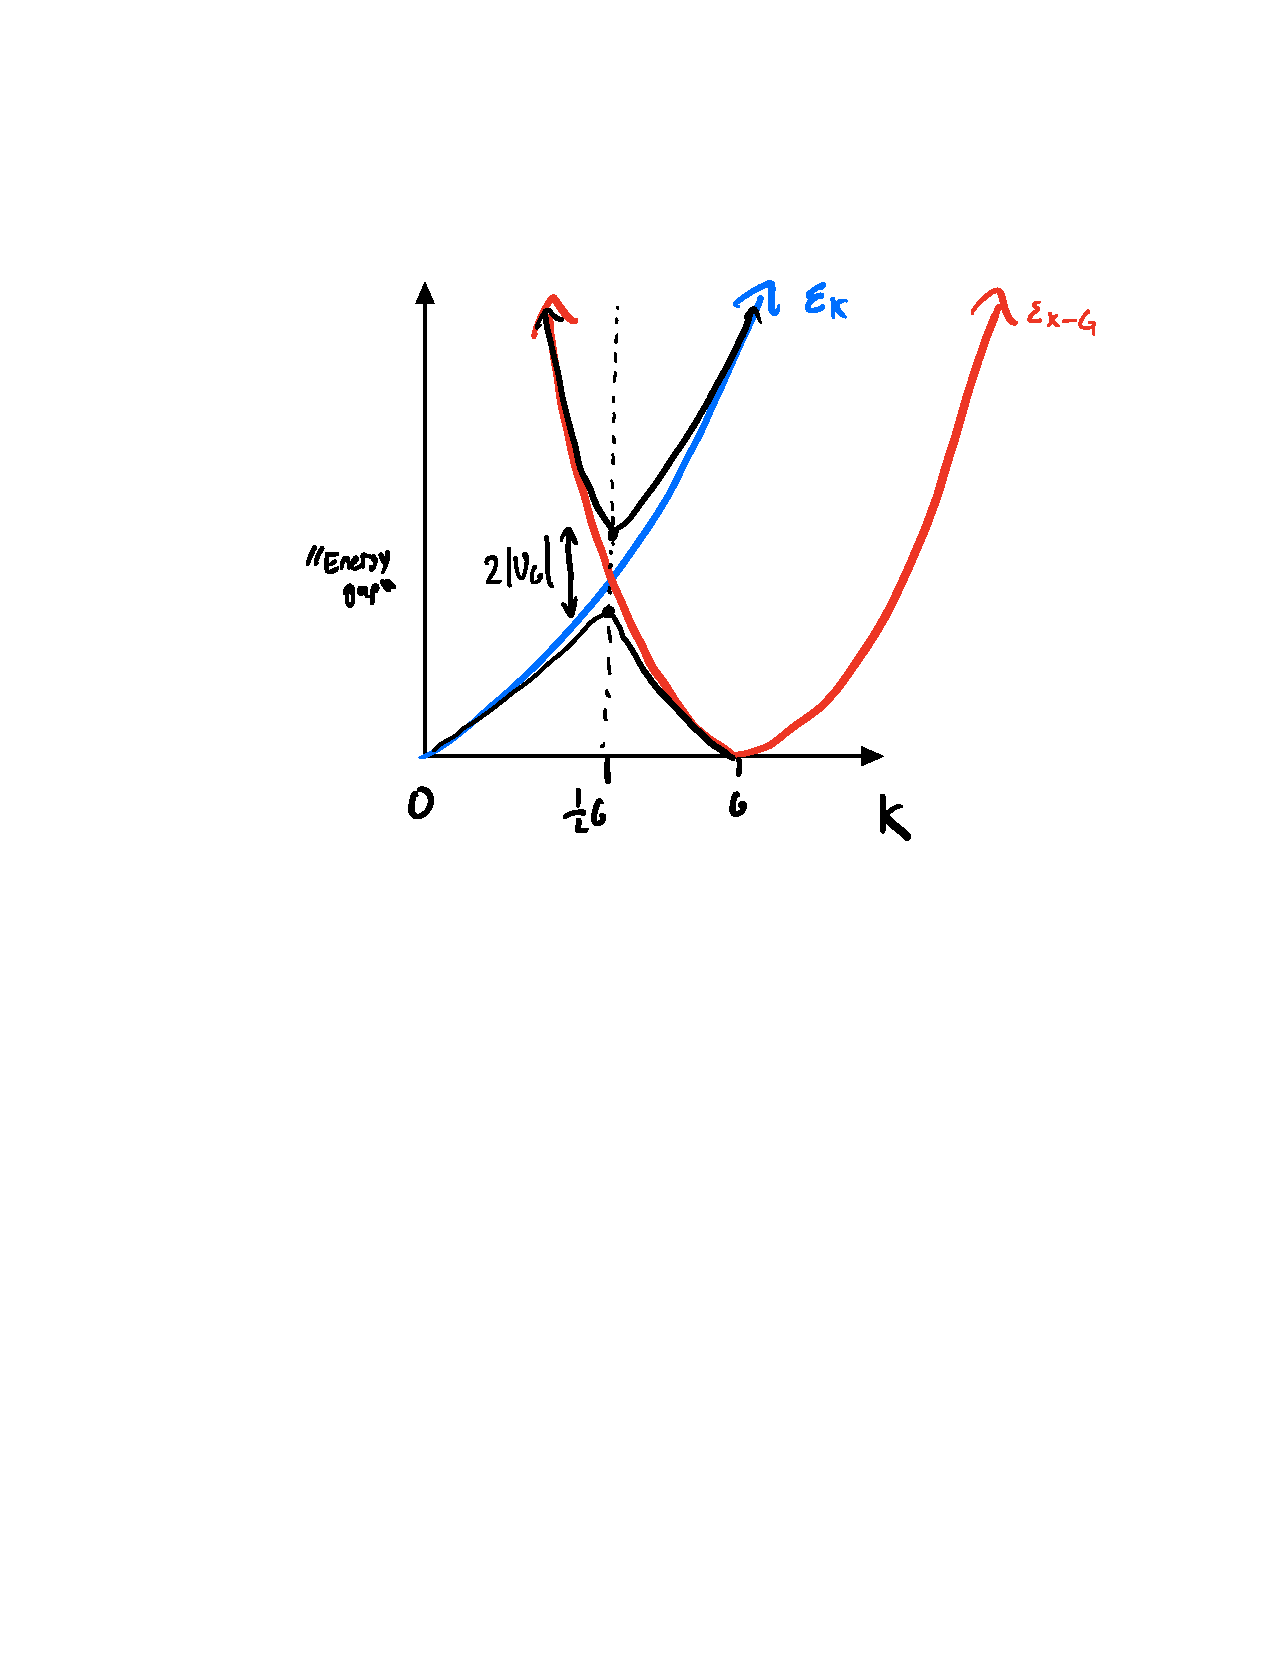
\includegraphics[scale=0.7]{Images/fig-energyvskgap.pdf}
    
    \caption{Plot of the energy $\e_k$ and $\e_{k-G}$ as a function of $k$. At $k = \frac{1}{2}G$ the two energy functions coincide. At and near this point, non-degenerate perturbation theory breaks down. A more careful treatment using degenerate perturbation theory shows that there are two energy levels, separated by a gap $2\abs{U_G}$.}
    \label{fig-energyvskgap}
\end{figure}
\newpage
\section{Electrons in a Periodic Potential: Band Theory of Solids}

\subsection{Review: Bloch's Theorem}
See A\&M Ch. 8 for proof(s) and extended discussion.

\textbf{Theorem (Bloch).} Consider the eigenstates $\psi$ of the one-electron Hamiltonian:
\begin{align*}
    H = \frac{\hbar^2\nabla^2}{2m} + U(\v{r})
\end{align*}
where $U(\v{r} + \v{R}) = U(\v{r})$ for all $\v{R}$ in the Bravais lattice. These eigenstates can be chosen to have the form:
\begin{equation}\label{eq-Blocheigenstates}
    \boxed{\psi_{nk}(\v{r}) = e^{i\v{k}\cdot \v{r}}\mu_{nk}(\v{r})}
\end{equation}
where:
\begin{equation}\label{eq-Blocheigenstatesperiodic}
    \mu_{nk}(\v{r} + \v{R}) = \mu_{nu}(\v{r})
\end{equation} 

The interesting part of this statement is that even though the Haniltonian has a full symmetry under translation by $+ \v{R}$. The eigenstates do not; there is a part that possesses the symmetry $\mu_{nk}(\v{r})$ and a part that does not, $e^{i\v{k} \cdot \v{r}}$ which is translation invariant. This should not be totally unexpected; for example the QHO is symmetric under inversion, but the wavefunctions do not have all of this symmetry ($n$ even is even, $n$ odd is odd).

A remark: Note that Eqs. \eqref{eq-Blocheigenstates} and \eqref{eq-Blocheigenstatesperiodic} imply that:
\begin{equation}
    \psi_{nk}(\v{r} + \v{R}) = e^{i\v{k} \cdot \v{R}}\psi_{nk}(\v{r}).
\end{equation}

In Eq. \eqref{eq-Blocheigenstates}, $\v{k}$ is known as a crystal momentum and $n$ is the band index. In free space, complete translation invariance implies the conservation of momentum. In a lattice, we have translation invariance w.r.t the Bravais lattice $\v{R}$, only, which implies that momentum is not conserved, but the crystal momentum is conserved.

\subsection{Weak Periodic Potential}
This is also known as ``nearly free'' electrons in a periodic lattice. We consider the same Hamiltonian $H = \frac{\hbar^2\nabla^2}{2m} + U(\v{r})$ where $U(\v{r})$ is ``weak'', sufficiently weak enough to be treated in perturbation theory. We call $H_0 = \frac{\hbar^2\nabla^2}{2m}$ and $H' = U(\v{r})$.

First, we transform $H$ into second-quantized notation:
\begin{equation}
    \begin{split}
        H_0 &= \sum_{\v{k}, \sigma} \e_\v{k}c^\dag_{\v{k}\sigma}c_{\v{k}\sigma}, \quad \e_\v{k} = \frac{\hbar^2\v{k}^2}{2m}
        \\ H' &= \sum_{\v{k}\v{k}'\sigma\sigma'}\bra{\v{k}\sigma}U\ket{\v{k}'\sigma}c_{\v{k}\sigma}^\dag c_{\v{k}'\sigma'}
    \end{split}
\end{equation}
where we note that as usual we work in the plane wave basis $\psi_\v{k} = \frac{1}{\sqrt{V}}e^{i\v{k} \cdot \v{r}}$, and so:
\begin{equation}
    \sum_{\v{k}\v{k}'\sigma\sigma'}\bra{\v{k}\sigma}U\ket{\v{k}'\sigma} = \frac{1}{V}\delta_{\sigma\sigma'}\int d^3 r e^{-i\v{r}\cdot(\v{k} - \v{k}')}U(\v{r})
\end{equation}
Note that due to its periodic property, $U$ can be written as:
\begin{equation}
    U(\v{r}) = \sum_{\v{G}}e^{i\v{r} \cdot \v{G}}U_\v{G}
\end{equation}
where $\v{G}$ are reciprocal lattice vectors satisfying $e^{i\v{G} \cdot \v{R}} = 1$ for all $\v{R}$ in the Bravais lattice (check)! $U_\v{G}$ is the fourier transform of our potential, evaluated at $\v{G}$.

We further assume that $U_{\v{G} = 0} = 0$, which only redefines the overall energy zero. We can therefore write:
\begin{equation}
    \bra{\v{k}\sigma}U\ket{\v{k}'\sigma'} = \frac{\delta_{\sigma\sigma'}}{V} \int d^3r \sum_\v{G} U_\v{G} e^{-i\v{r}\cdot(\v{k} - \v{k'} - \v{G})} = \delta_{\sigma\sigma'}\sum_\v{G}U_\v{G}\delta_{\v{k} - \v{k}', \v{G}}
\end{equation}
when the dust settles, we find:
\begin{equation}
    H' = \sum_{\v{k}\v{G}\sigma} U_\v{G} c^\dag_{\v{k} + \v{G}\sigma}c_{\v{k}\sigma}
\end{equation}
which is a very suggestive rewrite; for each term corresponds to the destruction of an electron with wavevector $\v{k}$ and the creation of an electron with wavevector $\v{k} + \v{G}$. This also explains the conservation of crystal momentum; the electron undergoes scattering processes which changes the momentum from $\v{k}$ to $\v{k} + \v{G}$ (so momentum is not conserved) but the crystal momentum (i.e. momentum up to reciprocal lattice vectors) is. This also connects back to the Bruillion zone; the wavevector $\v{k}$ appearing here can always be confined to the first Bruillion zone.

In the following, we suppress the spin index, and focus on 1D systems for simplicity. So, we have:
\begin{align*}
    H_0 = \sum_k \e_k c^\dag_k c_k, \quad H' = \sum_{k, G} U_G c^\dag_{k + G}c_k
\end{align*}
we ask how is an electron in an eigenstates $\ket{k} = c^\dag_k \ket{0}$ of $H_0$ perturbed by $H'$.

\subsubsection{Zeroth-order perturbation theory}
To start, in zeroth order perturabtion theory, we have:
\begin{equation}
    E_k^{(0)} = \e_k
\end{equation}
Of course, nothing exciting here...

\subsubsection{First-order perturbation theory}
We have:
\begin{equation}
    E_k^{(1)} = \bra{k}H'\ket{k} = \bra{k}\sum_{q,G} U_G c^\dag_{q + G}c_q\ket{k} = \bra{k}\sum_G U_G c_{k+G}^\dag \ket{0} = \sum_G U_G\braket{k}{k+G} = U_0 = 0.
\end{equation}
so the first order contribution is zero.

\subsubsection{Second-order perturbation theory}
We have:
\begin{equation}
    E_k^{(2)} = \sum_{k' \neq k} \frac{\abs{\bra{k}H'\ket{k'}}^2}{\e_{k'} - \e_k}
\end{equation}
So we calculate:
\begin{equation}
    \bra{k}H'\ket{k'} = \sum_{qG}U_G\bra{k}c^\dag_{q + G}c_q \ket{k'} = \sum_G U_G\bra{k}c^\dag_{k'+G}\ket{0} = \sum_G U_G\braket{k}{k'+G} = \sum_G U_G \delta_{k, k'+G} = 
\end{equation}
Therefore:
\begin{equation}
    E_k^{(2)} = \sum_{k' \neq k, G, G'}\frac{U_G U_{G'}^* \delta_{k,k'+G}\delta_{k, k'+G'}}{\e_{k'} - \e_k} = \sum_{G \neq 0,G'} \frac{U_G U_{G'}^* \delta_{GG'}}{\e_{k+G} - \e_k} = \sum_{G \neq 0} \frac{\abs{U_G}^2}{\e_{k+G} - \e_k}
\end{equation}

\begin{figure}[htbp]
    \centering
    
    \caption{<caption>}
    \label{<label>}
\end{figure}

For small $\abs{U_G}$, this correction is small, EXCEPT when $\abs{\e_{k - G} - \e_k}$ is also small. This occurs at specific values of $\v{k} = \frac{1}{2}\v{G}$ (valid also in 3D). However this is not the final answer; in reality there will not be an infinite correction. What's the catch? When we do perturbation theory as we have, we assume that the energy levels are non-degenerate; but here there is a degeneracy. Hence, at and near $\v{k} = \frac{1}{2}\v{G}$, we must apply degenerate perturbation theory because $\e_{k - G} = \e_k$ and this could be viewed as a degeneracy.

\subsection{Degenerate Perturbation Theory}
We define two near degenerate states:
\begin{equation}
    \ket{1} = \ket{k}, \quad \ket{2} = \ket{k - G_1}
\end{equation}
and construct the Hamiltonian matrix in this basis:
\begin{equation}
    H = \m{\bra{1}H\ket{1} & \bra{1}H\ket{2} \\ \bra{2}H\ket{1} & \bra{2}H\ket{2}} = \m{\e_k & U_G \\ U_G^* & \e_{k-G}}
\end{equation}
The perturbed energies are given by eigenvalues:
\begin{equation}
    \det\m{\e_k - E & U_G \\ U_G^* & \e_{k-G} - E} = 0 \implies (\e_k - E)(\e_{k-G} - E) - \abs{U_G}^2 = 0
\end{equation}
so then:
\begin{equation}
    E_k = \frac{1}{2}\left(\e_k + \e_{k-G}\right) \pm \sqrt{\frac{1}{4}\left(\e_k - \e_{k-G}\right)^2 + \abs{U_G}^2}
\end{equation}
Note for $k = \frac{1}{2}G$, i.e. the degeneracy point, this implies:
\begin{equation}
    E_k = \e_k \pm \abs{U_G}.
\end{equation}
So we have an energy gap! This quantifies the distinction of metals and insulators, using quantum mechanics; we will go further into this discussion next class.
\newpage
\section{Density Functional Theory}

\subsection{Motivation}
A brief recap - at the beginning of the term we discussed the Jellium model, where we replaced the ionic lattice with a uniform positive background, and we then calculated the energy of electrons amongst other properties. We then began to discuss electrons moving in a periodic potential of the lattice, which lead to band structure theory - but in this approximation we neglected interactions between the electrons. In a real solid that we have both a periodic lattice and electronic interactions. Trying to combine the two leads to an intractable problem, as as soon as we abandon the independent electron approximation, suddenly the wavefunction becomes a function of $10^{23}$ variables, and there is no good method to get this wavefunction in a system that does not have full translational invariance.

DFT is then the only practical way to perform calculations for electrons structure in real solids. It was developed bhy Walter Kohn in the 60s. We briefly survey the topic in a single class today, but there exist entire books written on the topic and it is a technique well-used in research today.

\subsection{The Hohenberg-Kohn Theorem}

QFT is grounded in the Hohenberg-Kohn theorem, which applies to the family of electron Hamiltonians of the form:
\begin{equation}\label{eq-DFTHamiltonian}
    \hat{H} = \sum_{\v{k}, \sigma} \frac{\hbar\v{k}^2}{2m}c_{\v{k}\sigma}^\dag c_{\v{k}\sigma} + \sum_{\v{k}, \v{q}, \sigma}U(\v{q})c^\dag_{\v{k} + \v{q}, \sigma}c_{\v{k}\sigma} + \frac{1}{2}\sum_{\v{k}\v{p}\v{q}\sigma\sigma'}V_\v{q}c^\dag_{\v{k}-\v{q}\sigma}c^\dag_{\v{p}+\v{q}\sigma'}c_{\v{p}\sigma'}c_{\v{k}\sigma}
\end{equation}
where the first term is the electron kinetic energy which we call $\hat{T}$, the second term is the potential term $\hat{U}$, and the third term is the Coulomb interactions $\hat{V}$. 

The Hohenberg-Kohn theorem says that the expectation value of any operator $\hat{O}$ is a unique functional of the ground-state electron density $n_0(\v{r})$. We don't need the full many-body wavefunction of the system; we only need the ground state electron density. Quite incredible! From this theorem unfolds the apparatus of DFT. the simplification is that the density is a function only of three spatial variables $\v{r} = (r_x, r_y, r_z)$. We only need to couch calcualtions in terms of 3 variables, not $10^{23}$!

Comment: There do exist extensions of the theorem to thermal ensembles at finite temperature, though the HK theorem in the above form only addresses the ground state.

A few other remarks. The $\hat{T}, \hat{V}$ pieces of Eq. \eqref{eq-DFTHamiltonian} are universal across solids, and $\hat{U}$ is the only part that differs between solids. In principle, given $\hat{U}$ we can calcualte the electron density $n_0(\v{r})$. 

The HK theorem states that the mapping:
\begin{equation}
    U(\v{r}) \leftrightarrow n_0(\v{r})
\end{equation}
is actually reversible. Because from $U(\v{r})$ we can in principle obtain the full many-body wavefunction $\psi(\v{r}_1, \ldots, \v{r}_n)$ (and thus the expectation value $\avg{\hat{O}}$) this implies that $\avg{\hat{O}}$ is uniquely determined by $n_0(\v{r})$. Also note that everything we will say is true of non-degenerate ground states (degeneracy can add complications to these uniqueness statements), though we can extend the results to the case with degeneracy.

\subsection{Proof of the Hohenberg-Kohn Theorem}

\subsubsection{Part 1}
We first show that two potentials $U(\v{r})$ and $U'(\v{r})$ that differ by more than a trivial constant, necessarily lead to different ground states $\psi_0 \neq \psi_0'$. We have:
\begin{equation}
    \begin{split}
        &(\hat{T} + \hat{V} + \hat{U})\psi_0 = \e_0\psi_0
        \\ &(\hat{T} + \hat{V} + \hat{U}')\psi_0' = \e_0'\psi_0'
    \end{split}
\end{equation}
We proceed by proof by contradiction. Assume $\psi_0 = \psi_0'$, then subtracting the second equation from the first:
\begin{equation}
    (\hat{U} - \hat{U}')\psi_- = (\e_0 - \e_0')\psi_0
\end{equation}
So $\hat{U}, \hat{U}'$ only differ by a trivial constant, contradicting our assertion that they differ by more than a trivial constant. \qed

\subsubsection{Part 2}
It is also clear that two different densities $n_0(\v{r}) \neq n_0'(\v{r})$ require different potentials - this follows from the uniqueness of solutions to the Schrodinger equation (in the non-degenerate case). 

It therefore follows that the ground state wavefunction is uniquely specified by the electron density. One can also show that $\psi_0 \neq \psi_0'$ implies $n_0(\v{r}) \neq n_0'(\v{r}')$ which completes the proof. \qed

\subsection{Variational Principle}
There is an important variational principle associated with the HK theorem. HK applies for expectation values of all operators, so in particular let us pick the Hamiltonian (i.e. the ground state energy):
\begin{equation}
    \e[n] = \bra{\psi_0[n]}\hat{T} + \hat{V} + \hat{U}\ket{\psi_0[n]}
\end{equation}
where $\e[n]$ is the ground state energy functional, such that $\e_0 = \e[n_0]$ is the true ground state energy. As a refresher, a functional is a mapping from the space of functions to the space of numbers. For example the definite integral over $[0, 1]$ is a functional. We distinguish them by angular brackets, and their arguments are functions. 

It then holds that:
\begin{equation}
    \e_0 < \e[n]
\end{equation}
for any $n(\v{r}) \neq n_0(\v{r})$. This is nothing more than a restatement of the familiar variational principle of $E_0 \leq \bra{\psi}H\ket{\psi}$. 


This variational principle gives the practical machinery for doing DFT calcualtions; the ground state energy and $n_0(\v{r})$ can be found by minimizing this functional. $\e[n]$ is usually written as:
\begin{equation}
    \e[n] = F_{HK}[n] + \int d^3rn(\v{r})U(\v{r})
\end{equation}
where $F_{HK}[n] = \bra{\psi_0[n]}\hat{T} + \hat{V}\ket{\psi_0[n]}$, which importantly is the same for all systems on the account of universality! $F_{HK}$ has to be determined only once! Of course anything that is this useful is not so easily obtained, and various DFT approaches differ in what they use for the $F_{HK}$ functional. Let us explain the second term - why can it be written as the simple integral? First, we write:
\begin{align*}
    n(\v{r}) = \int \set{d^3r} \psi^*(\v{r}_1, \ldots \v{r}_N)\sum_{i=1}^N \delta(\v{r} - \v{r}_i)\psi(\v{r}_1 \ldots \v{r}_N)
\end{align*}
Where $\set{d^3r} = d^3r_1\ldots d^3r_N$. Then:
\begin{equation}
    \bra{\psi_0}U\ket{\psi_0} = \int \set{d^3r}\psi^*(\v{r}_1, \ldots \v{r}_N)\sum_{i=1}^N U(\v{r}_i)\psi(\v{r}_1, \ldots \v{r}_N) = \int \set{d^3r} d^3r_p \psi^*(\ldots)\sum_i \delta(\v{r}_p - \v{r}_i)U(\v{r}_p)\psi(\ldots)
\end{equation}
and separating this into two integrals, and the integral over all wavefunction coordinates gives exactly $n(\v{r})$, giving precisely $ \bra{\psi_0}U\ket{\psi_0} = \int d^3rn(\v{r})U(\v{r})$.

\subsection{The Kohn-Sham Formulation}
This formulation allows for practical applications of the HK theorem. The idea - one imagines that there is a non-interacting reference system $\hat{H}_S = \hat{T} + \hat{U}_S$ whose potential $\hat{U}_S$ is chosen such that the ground state density is precisely the same as the actual interacting system $\hat{H} = \hat{T} + \hat{V} + \hat{U}$ we are interested in. Because computations of $\psi_0$ and $n_0$ are ``easy'' in a non-interacting system $\hat{H}_S$ (as the indepdendent electron approximation can be used), we can then practically implement this whole scheme.

\subsubsection{DFT for the Reference System}
Similarly for the actual system, we have a ground state energy function:
\begin{equation}
    \e_S[n] = T_s[n] + \int d^3rU_s(\v{r})n(\v{r})
\end{equation}
where here $n_s(\v{r})$ can be easily obtained from the wavefunctions:
\begin{equation}\label{eq-nrDFT}
    n_s(\v{r}) = \sum_{i=1}^N \abs{\phi_i(\v{r})}^2
\end{equation}
and we solve for the $\phi_i$s by solving the Schrodinger equation:
\begin{equation}\label{eq-SEDFT}
    \left[-\frac{\hbar^2\nabla^2}{2m} + U_S(\v{r})\right]\phi_i(\v{r}) = \e_i\phi_i(\v{r})
\end{equation}
The hard part is we do not know what $U_S$ is - we need to find its form. We write down again the ground state energy functional for the full system, but in a peculiar way:
\begin{equation}
    \begin{split}
        \e[n] &= T[n] + V[n] + \int d^3rn(\v{r})U(\v{r}) \\ &= T_S[n] + \left[T[n] - T_S[n] - \frac{e^2}{2}\int d^3r d^3r' \frac{n(\v{r})n(\v{r}')}{\abs{\v{r} - \v{r}'}}\right] + \frac{e}{2}\int d^3rd^3r' \frac{n(\v{r})n(\v{r}')}{\abs{\v{r} - \v{r}'}} + \int d^3rU(\v{r})n(\v{r})
    \end{split}
\end{equation}
Where the term in brackets is the exchange-correlation functional:
\begin{equation}
    \e_{xc}[n] = F_{HK}[n] - \frac{e^2}{2}\int d^3rd^3r'\frac{n(\v{r})n(\v{r}')}{\abs{\v{r} - \v{r}'}} - T_S[n]
\end{equation}
We minimize $\e[n]$ by variational calculus:
\begin{equation}\label{eq-fullEminimization}
    0 = \frac{\delta \e[n]}{\delta n(\v{r})} = \frac{\delta T_s[n]}{\delta n(\v{r})} + e^2 \int d^3r'\frac{n(\v{r}')}{\abs{\v{r} - \v{r}'}} + U(\v{r}) + v_{xc}[n(\v{r})]
\end{equation}
where $v_{xc}[n(\v{r})] = \frac{\delta \e_{xc}[n]}{\delta n(\v{r})}$ is the exchange-correlation potential. We minimize the reference system:
\begin{equation}
    0 = \frac{\delta \e_n[n]}{\delta n(\v{r})} = \frac{\delta T_s}{n(\v{r})} + U_S(\v{r})
\end{equation}
and then subtracting from the minimization of the full system in Eq. \eqref{eq-fullEminimization}:
\begin{equation}\label{eq-Us}
    U_s(\v{r}) = U(\v{r}) + e^2\int d^3r'\frac{n(\v{r}')}{\abs{\v{r} - \v{r}'}} + v_{xc}(\v{r})
\end{equation}
This is the important result! In practical calculations we can therefore implement Kohn-Sham by following the three-step program:
\begin{enumerate}
    \item Choose an initial trial density $n(\v{r})$. Substitute in Eq. \eqref{eq-Us} and calculate $U_S(\v{r})$. 
    \item Solve the SE in Eq. \eqref{eq-SEDFT} for $\phi_i(\v{r})$ and find the new density $n(\v{r})$ from Eq. \eqref{eq-nrDFT}
    \item Iterate until $n(\v{r})$ stops changing.
\end{enumerate}
The enormous advantage of this procedure is that at no point in this calculation are we ever forced to calculate the full many-body wavefunction. Of course, it comes at a cost - we have hidden all of the interaction physics inside of the exchange-correlation potential $v_{xc}$. Despite this - DFT remains as one of the most successful techniques in CM physics today, and is the basis for much of our understanding of solids.

\subsubsection{Remarks}
\begin{enumerate}[(i)]
    \item The above procedure is implemented in various software packages (Wien 2K, Quantum Espresso...)
    \item These differ mainly in the form of $v_{xc}$. 
    \item Packages provide ``band structures'', i.e. energy eigenvalues $\e_i(\v{k})$ of Eq. \eqref{eq-SEDFT}. If we construct the full many-body wavefunctions from the obtained observable expectation values, we often obtain very good approximations to the true systems - and systems for which DFT fail are unusual/interesting.
    \item There are many useful generalizations of DFT, such as TD-DFT which adds time-dependence, CDFT (current DFT) which includes an external magnetic field, and EDFT (ensemble DFT) which deals with degeneracies.
\end{enumerate}

\subsection{Choices for the Exchange-Correlation Potential}
Many sophisticated approximations for $\e_{xc}[n]$ have been developed and implemented over the years. 

The simplest such is the local density approximation, which assumes that $\e_{xc}$ only depends on the local density:
\begin{equation}
    \e_{xc}[n] = \int d^3r n(\v{r})\e_{xc}(n(\v{r}))
\end{equation}
where $\e_{xc}(n)$ is the exchange-correlation energy (per particle) of a homogenous electron gas of density $n$ (Jellium):
\begin{equation}
    \e_{xc}(n) = \frac{e^2}{a_0r_s^2}(br_s + cr_s\log r_s + \ldots).
\end{equation}
Other popular approximations include LSDA (low spin density approximation) and GGA, the ``generalized gradient approximation'':
\begin{equation}
    \e_{xc}[n] = \int d^3r[g_{00}(n) + g_{22}(n)(\nabla n)^2 + g_{42}(n)(\nabla^2 n)^2 + \ldots]
\end{equation}

Next time, we will start discussing the semiclassical theory of conduction in metals. Please read A\&M p214-218 in preparation.


\end{document}